\documentclass[11pt]{article}
\usepackage[spanish]{babel}
\usepackage[utf8]{inputenc}
\usepackage[T1]{fontenc}
\usepackage{lmodern}
\usepackage[margin=1in]{geometry}
\usepackage{graphicx}
\usepackage{float}
\usepackage{multirow}
\usepackage{array}
\usepackage{tabularx}
\usepackage{longtable}
\usepackage{enumitem}
\usepackage[unicode,hidelinks]{hyperref}

\setlist[itemize]{itemsep=0.35em, topsep=0.35em}

\title{Apunte resumen de Electrónica Digital 3}
\author{Juan Ignacio Cleri}
\date{\today}

\begin{document}

\maketitle
\tableofcontents

\section{Descripción}
\subsection{Introducción}
Este documento corresponde al apunte de la materia Electrónica Digital 3 y está centrado en el estudio del microprocesador LPC1769, basado en la arquitectura ARM Cortex-M3. Está pensado para aplicaciones embebidas y requiere un alto nivel de integración y bajo nivel de disipación de energía.

\subsection{Características}
\begin{itemize}
  \item CPU ARM Cortex-M3 de hasta 120 MHz con soporte de interrupciones (NVIC) y bajo consumo.
  \item Hasta 512 KB de flash y 64 KB de RAM, con aceleración para acceso rápido a código y datos.
  \item Periféricos de comunicación completos: Ethernet, USB 2.0 OTG, CAN, UART, SPI, SSP, I2C e I2S.
  \item Interfaces analógicas integradas: ADC de 12 bits, DAC de 10 bits y sensores/monitores internos.
  \item Temporización y control: timers de 32 bits, PWM, RTC de bajo consumo y watchdog.
  \item Entradas/salidas versátiles: GPIO de alta velocidad, captura/comparación y codificador en cuadratura.
  \item Enfoque en eficiencia energética con modos Sleep, Deep-sleep, Power-down y Deep power-down.
  \item Soporte de depuración y trazado: JTAG/SWD, ETM y emulación en tiempo real.
  \item Reloj flexible: oscilador interno/externo, PLL y \textit{clock output} para supervisión del sistema.
  \item Encapsulados LQFP y BGA compactos, orientados a aplicaciones embebidas industriales.
\end{itemize}

\setcounter{subsection}{4}
\subsection{Diagrama de bloques}
\begin{figure}[H]
  \centering
  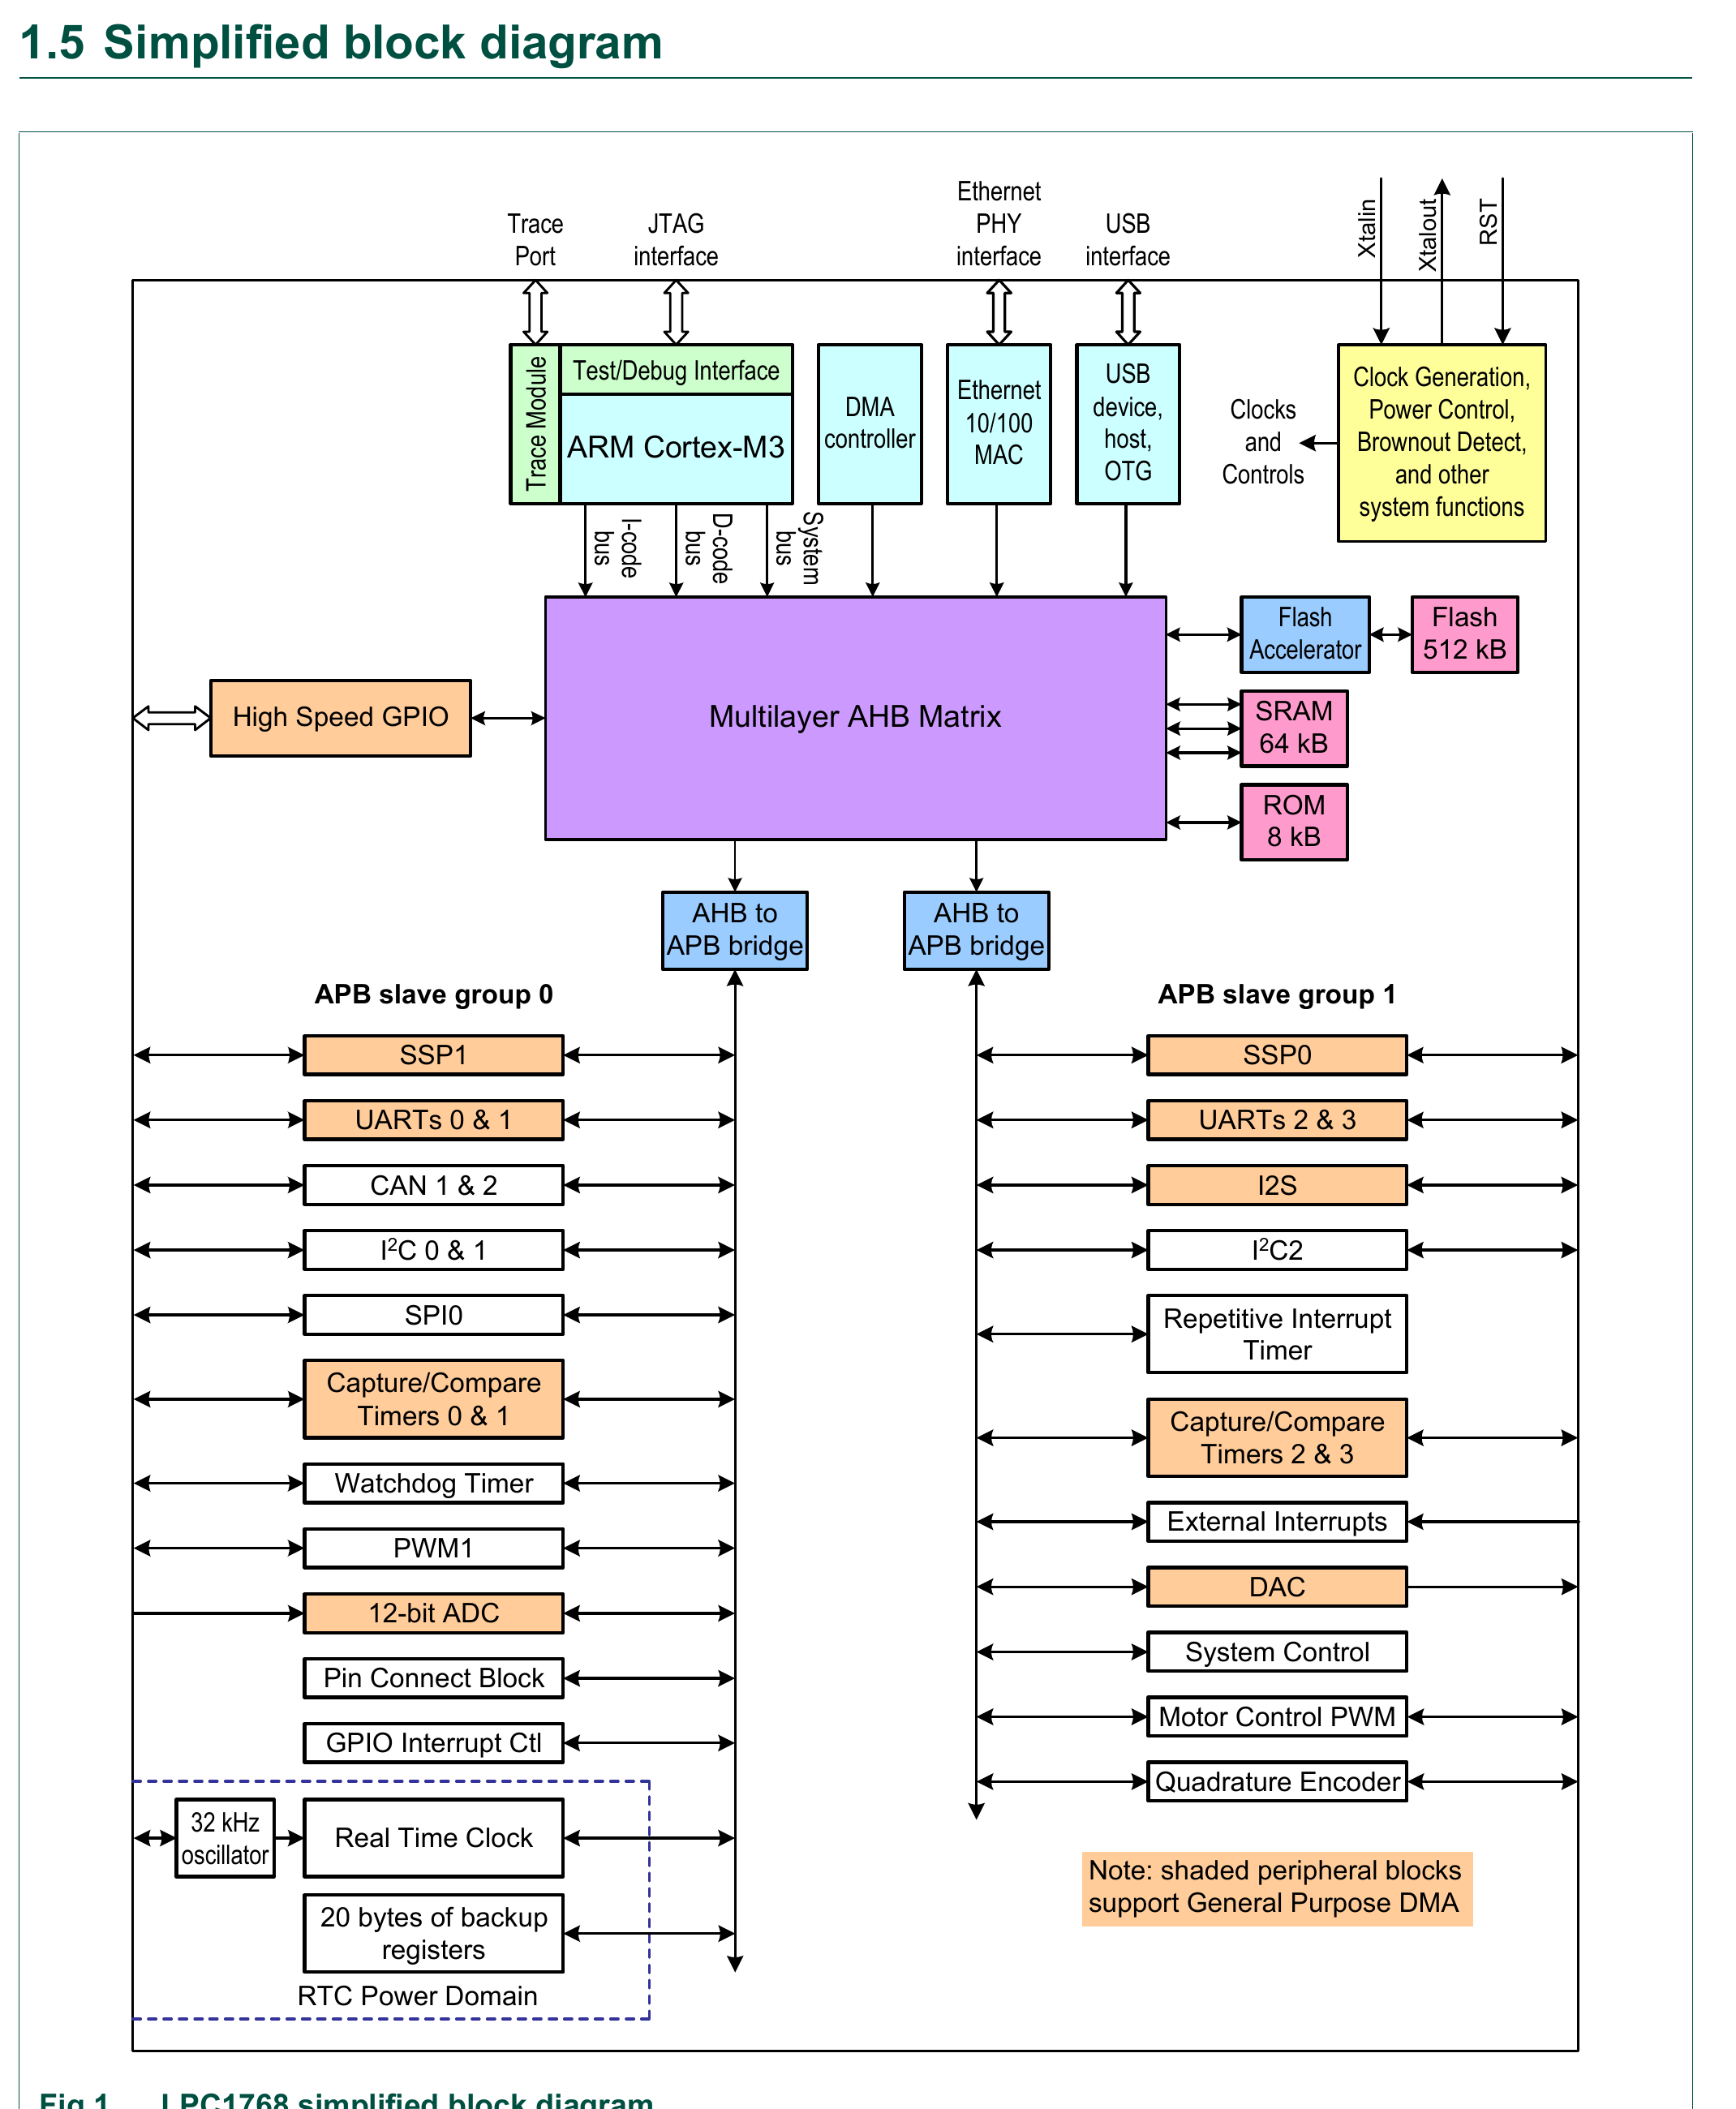
\includegraphics[width=0.93\textwidth]{images/lpc1769_block_diagram.png}
  \caption{Diagrama de bloques simplificado del LPC1769.}
\end{figure}

\subsection{Vista general de arquitectura}
\begin{figure}[H]
  \centering
  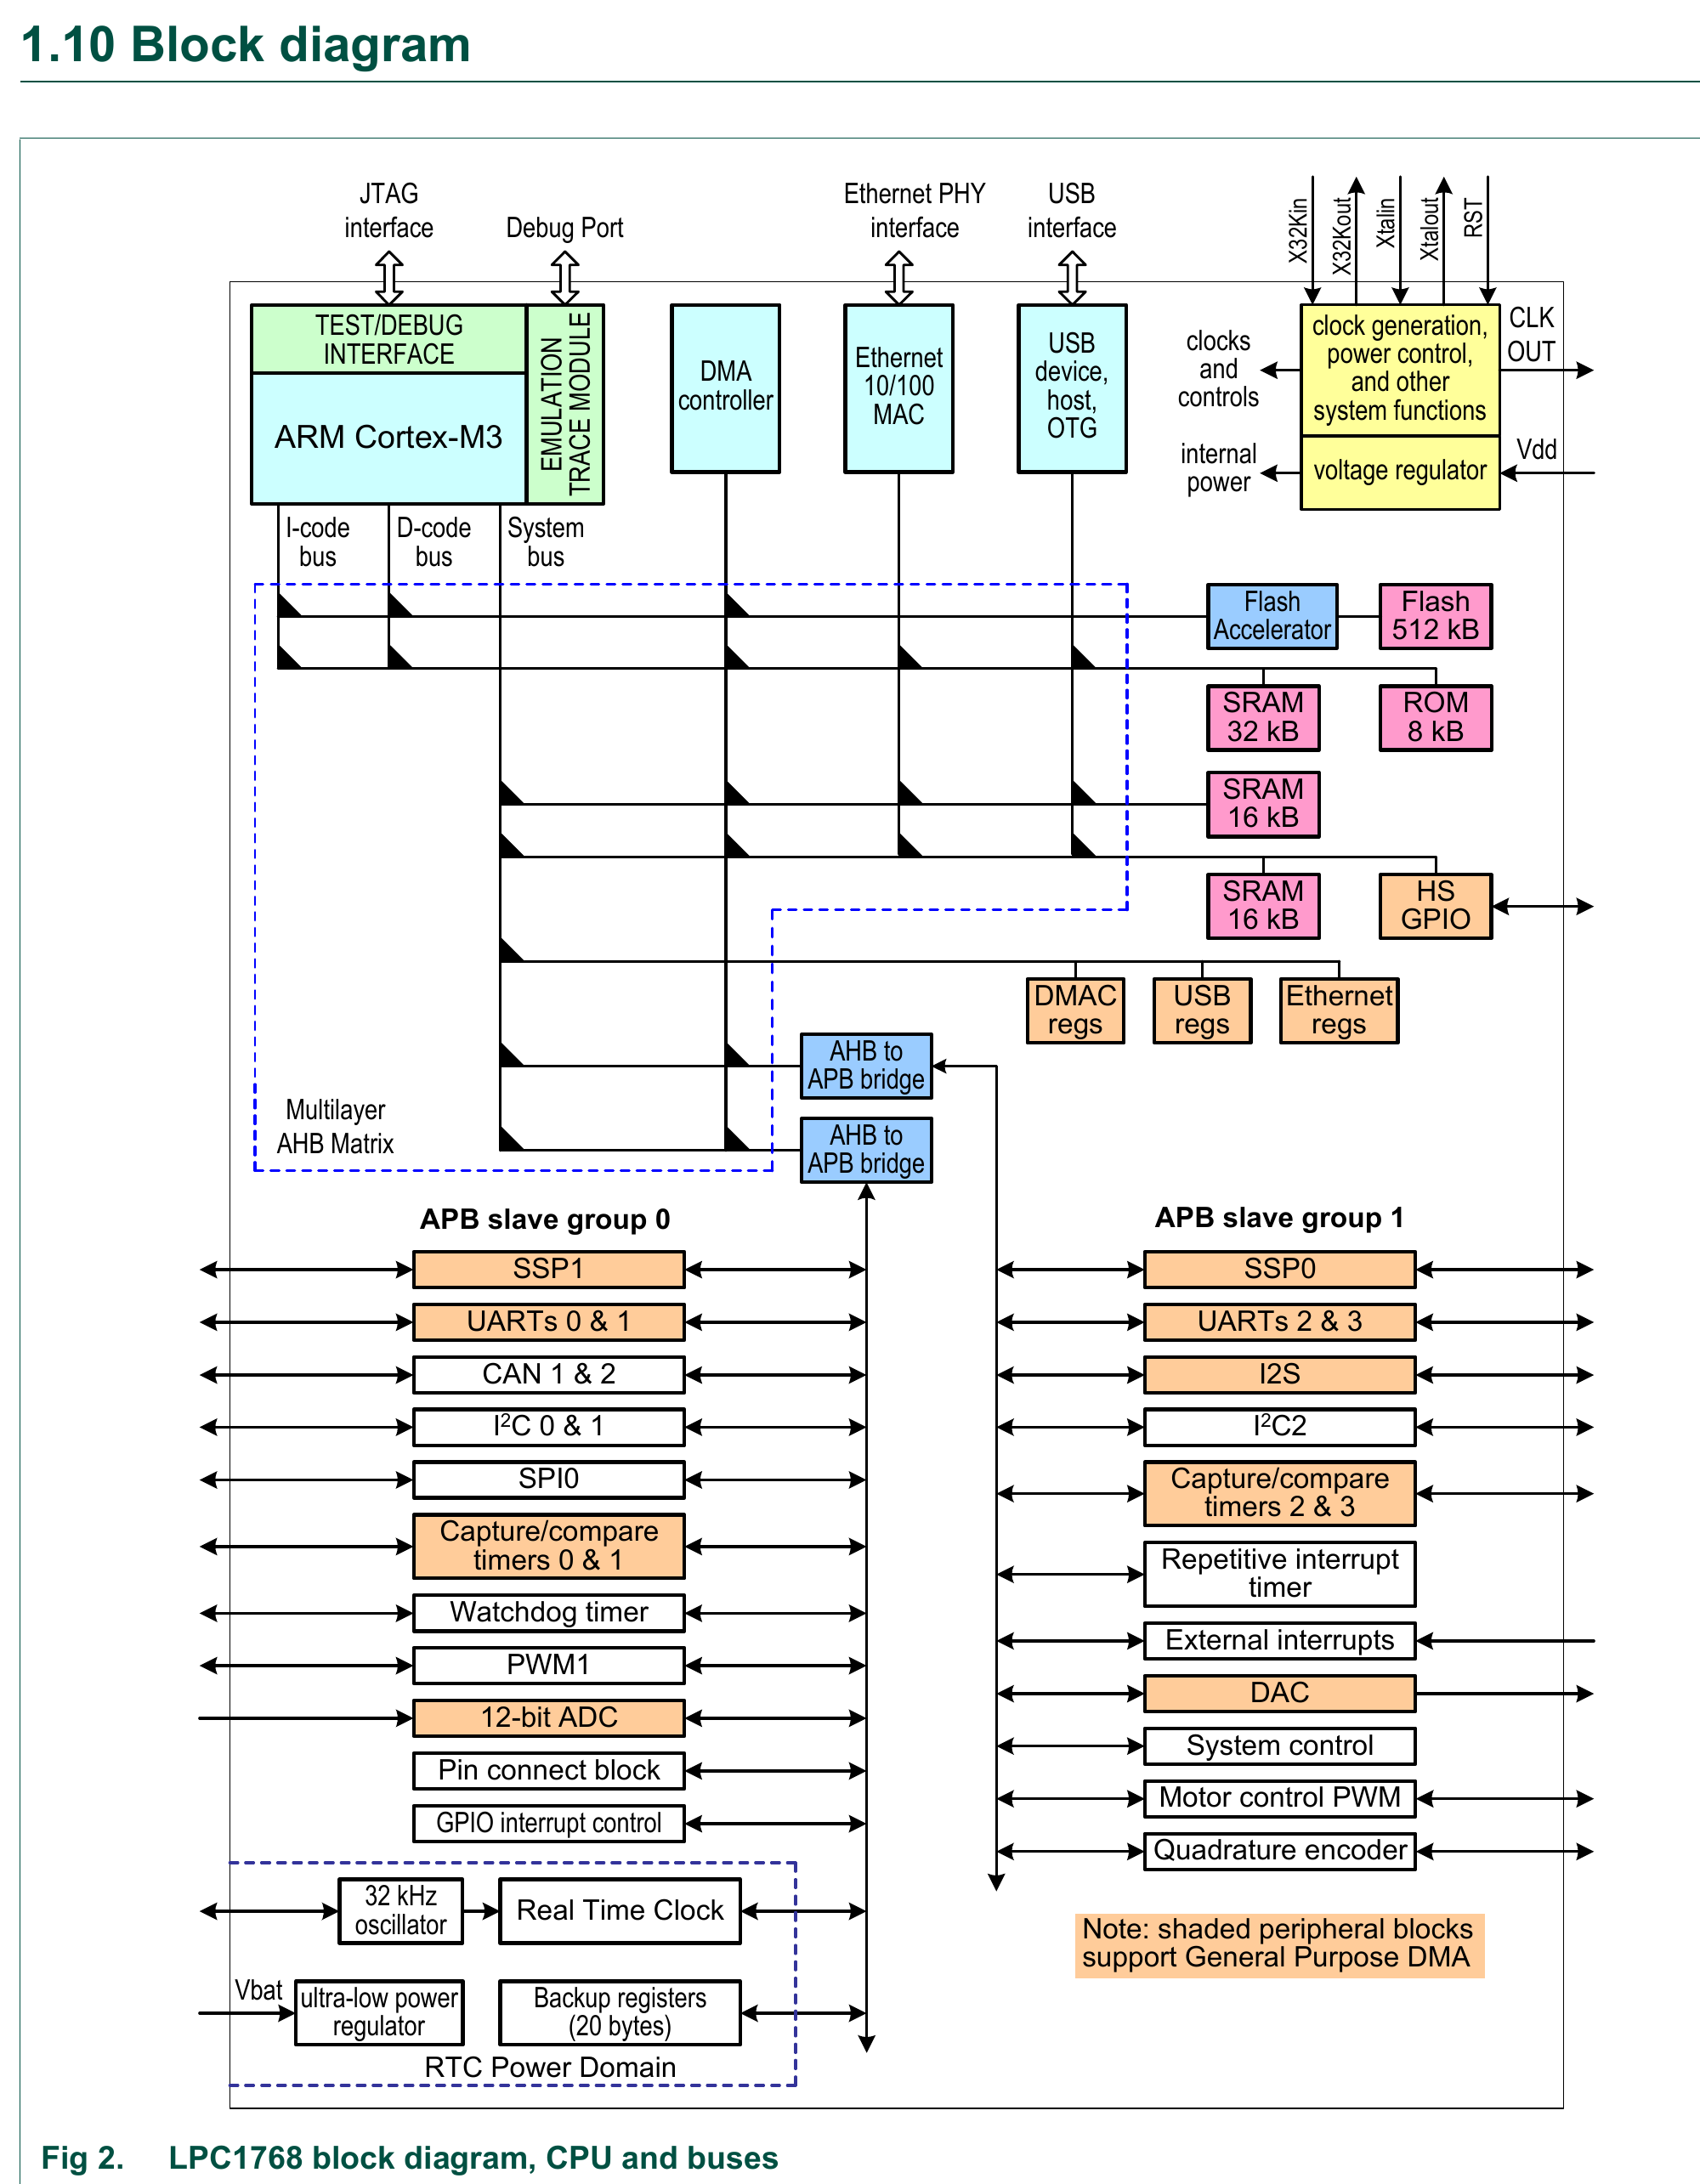
\includegraphics[width=0.83\textwidth]{images/lpc1769_ahb_matrix_detailed.png}
  \caption{Diagrama de bloques detallado con matriz AHB multicapa.}
\end{figure}

\begin{itemize}
  \item \textbf{Buses del núcleo ARM Cortex-M3:} El procesador usa tres buses AHB-Lite (\textit{Advanced High-performance Bus}): un bus de sistema y dos buses rápidos, \textbf{I-code} (instrucciones) y \textbf{D-code} (datos). Esta separación permite ejecutar accesos simultáneos cuando apuntan a periféricos distintos.

  \item \textbf{Matriz AHB multicapa:} El LPC17xx integra una matriz AHB multicapa que conecta los maestros de bus (CPU, DMA, Ethernet, USB, etc.) con distintos puertos esclavos. Así, varios accesos pueden ocurrir en paralelo y se mejora el rendimiento global.

  \item \textbf{Conexión de periféricos APB:} Los periféricos APB (\textit{Advanced Peripheral Bus}) se enlazan mediante dos buses APB conectados a puertos esclavos separados de la matriz AHB. Esto reduce colisiones entre CPU y DMA (Acceso Directo a Memoria).

  \item \textbf{Búfer de escritura APB:} Los puentes APB almacenan escrituras en búfer, permitiendo que la CPU o el DMA continúen su ejecución sin esperar a que cada escritura finalice.
\end{itemize}

\subsection{Opciones de configuración del Cortex-M3}
\begin{itemize}
  \item \textbf{Técnicas de segmentación (pipeline):} El núcleo aplica pipeline para mantener activos los bloques de procesamiento y memoria. En condiciones normales, mientras una instrucción se ejecuta, la siguiente se decodifica y una tercera se busca en memoria.

  \item \textbf{Versión del núcleo:} Los LPC17xx usan la versión \textbf{r2p0} del Cortex-M3, que integra opciones de sistema configurables:
  \begin{itemize}
    \item \textbf{NVIC (Nested Vectored Interrupt Controller):} controlador de interrupciones con temporizador SysTick.
    \item \textbf{WIC (Wakeup Interrupt Controller):} habilita un despertar más eficiente desde modos de bajo consumo.
    \item \textbf{MPU (Memory Protection Unit):} unidad de protección de memoria incorporada.
    \item \textbf{ROM Table:} expone a herramientas externas las direcciones de componentes de depuración.
  \end{itemize}

  \item \textbf{Opciones de depuración (Debug):} La CPU incorpora funciones configurables para diagnóstico y depuración de fallas, también asociadas al conjunto de opciones r2p0.
\end{itemize}

\subsection{Sistema de memoria flash en chip}
\begin{itemize}
  \item \textbf{Capacidad:} El LPC17xx integra hasta \textbf{512 kB de memoria flash} en el propio chip.
  \item \textbf{Rendimiento:} Incluye un \textbf{acelerador de flash} que mejora el acceso cuando trabaja junto con los buses rápidos AHB-Lite.
  \item \textbf{Uso:} La flash puede utilizarse tanto para \textbf{código} como para \textbf{datos}, aportando flexibilidad en aplicaciones embebidas.
  \item \textbf{Programación y actualización:} Puede programarse \textit{in-system} por puerto serie, y la propia aplicación puede \textbf{borrar/programar flash en ejecución}, facilitando actualizaciones de firmware en campo y almacenamiento de datos.
\end{itemize}

\subsection{Memoria SRAM en chip}
\begin{itemize}
  \item \textbf{32 kB de SRAM local:} conectada directamente a los buses locales de la CPU (I-code/D-code), lo que permite acceso de alta velocidad.
  \item \textbf{32 kB de SRAM AHB:} organizada en dos bloques de 16 kB y conectada al bus periférico AHB.
\end{itemize}

\section{Mapeo de memoria del LPC1769}
\subsection{Mapa de memoria y direccionamiento de periféricos}
\begin{table}[H]
  \centering
  \small
  \renewcommand{\arraystretch}{1.2}
  \setlength{\tabcolsep}{6pt}
  \caption{Uso de memoria y regiones del LPC1769}
  \begin{tabularx}{\textwidth}{|>{\raggedright\arraybackslash}p{0.22\textwidth}|>{\raggedright\arraybackslash}p{0.23\textwidth}|>{\raggedright\arraybackslash}X|}
    \hline
    \textbf{Rango de direcciones} & \textbf{Uso general} & \textbf{Detalle de región y descripción} \\
    \hline
    \multirow{3}{=}{\texttt{0x0000\,0000} a \\ \texttt{0x1FFF\,FFFF}}
      & Memoria no volátil en chip & 0x0000\,0000 -- 0x0007\,FFFF: para LPC1769 con 512 kB de memoria flash. \\
    \cline{2-3}
      & SRAM en chip & 0x1000\,0000 -- 0x1000\,7FFF: 32 kB de SRAM local. \\
    \cline{2-3}
      & Boot ROM & 0x1FFF\,0000 -- 0x1FFF\,1FFF: 8 kB de Boot ROM con servicios de flash. \\
    \hline
    \multirow{3}{=}{\texttt{0x2000\,0000} a \\ \texttt{0x3FFF\,FFFF}}
      & SRAM en chip (uso típico de datos periféricos) & 0x2007\,C000 -- 0x2007\,FFFF: banco AHB SRAM 0 (16 kB), presente en dispositivos con 32 kB o 64 kB de SRAM total. \\
    \cline{2-3}
      & SRAM en chip (uso típico de datos periféricos) & 0x2008\,0000 -- 0x2008\,3FFF: banco AHB SRAM 1 (16 kB), presente en dispositivos con 64 kB de SRAM total. \\
    \cline{2-3}
      & GPIO & 0x2009\,C000 -- 0x2009\,FFFF: registros GPIO. \\
    \hline
    \multirow{3}{=}{\texttt{0x4000\,0000} a \\ \texttt{0x5FFF\,FFFF}}
      & Periféricos APB & 0x4000\,0000 -- 0x4007\,FFFF: periféricos APB0, hasta 32 bloques de 16 kB cada uno. \\
    \cline{2-3}
      & Periféricos APB & 0x4008\,0000 -- 0x400F\,FFFF: periféricos APB1, hasta 32 bloques de 16 kB cada uno. \\
    \cline{2-3}
      & Periféricos AHB & 0x5000\,0000 -- 0x501F\,FFFF: controlador DMA, interfaz Ethernet e interfaz USB. \\
    \hline
    \texttt{0xE000\,0000} a \\ \texttt{0xE00F\,FFFF}
      & Bus de periféricos privados del Cortex-M3 & 0xE000\,0000 -- 0xE00F\,FFFF: funciones del Cortex-M3, incluido NVIC y temporizador SysTick. \\
    \hline
  \end{tabularx}
\end{table}

\subsection{Mapa de memoria}
\begin{figure}[H]
  \centering
  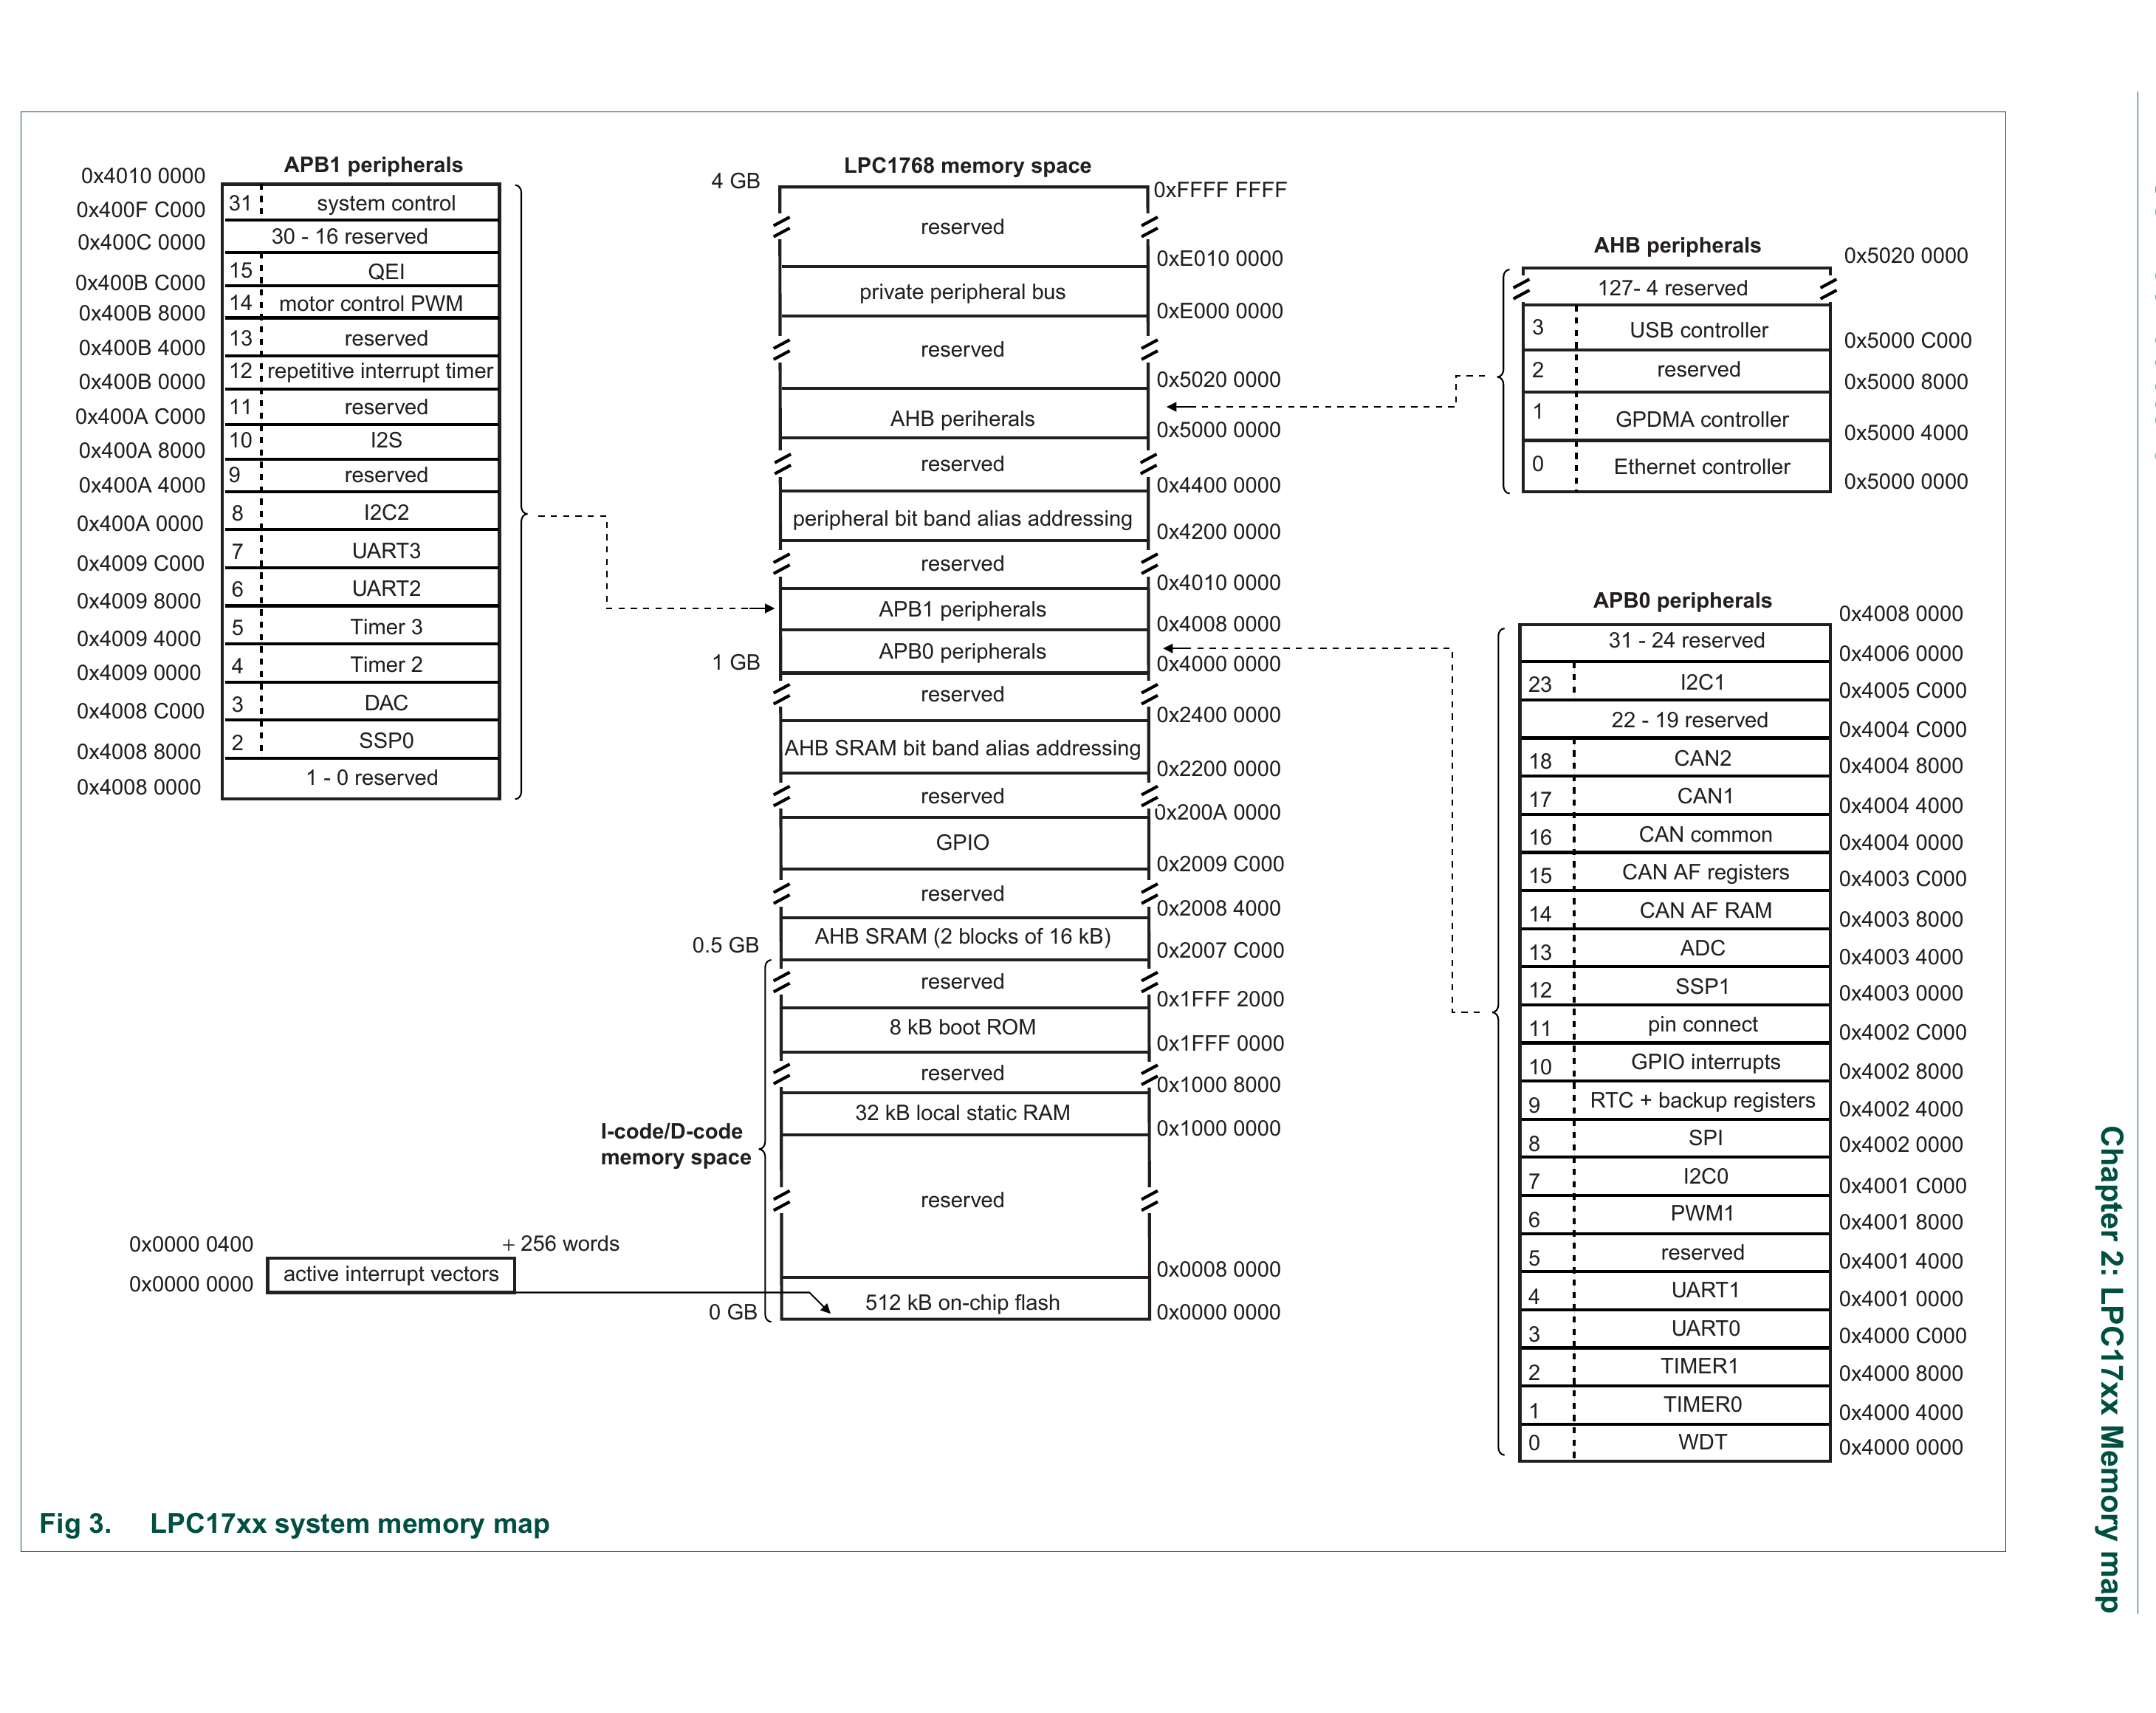
\includegraphics[width=0.98\textwidth]{images/lpc17xx_system_memory_map.png}
  \caption{Mapa de memoria del sistema LPC17xx.}
\end{figure}

\subsection{Direcciones de periféricos APB}
En esta sección se resume el mapeo de direcciones base de los periféricos conectados a los buses \textbf{APB0} y \textbf{APB1}. Cada bloque APB ocupa un espacio de \textbf{16 kB} y, en general, los registros de cada periférico no utilizan todo ese rango. Por este motivo, en varios casos aparecen direcciones \textit{aliasadas} o repetidas dentro del mismo bloque de 16 kB.

\begin{table}[H]
  \centering
  \small
  \renewcommand{\arraystretch}{1.1}
  \setlength{\tabcolsep}{4pt}
  \caption{Periféricos APB0 y direcciones base}
  \begin{tabularx}{0.94\textwidth}{|>{\raggedright\arraybackslash}p{0.14\textwidth}|>{\raggedright\arraybackslash}p{0.20\textwidth}|>{\raggedright\arraybackslash}X|}
    \hline
    \textbf{Periférico APB0} & \textbf{Dirección base} & \textbf{Nombre del periférico} \\
    \hline
    0 & \texttt{0x4000\,0000} & Watchdog timer (WDT) \\
    1 & \texttt{0x4000\,4000} & Timer 0 \\
    2 & \texttt{0x4000\,8000} & Timer 1 \\
    3 & \texttt{0x4000\,C000} & UART0 \\
    4 & \texttt{0x4001\,0000} & UART1 \\
    5 & \texttt{0x4001\,4000} & Reservado \\
    6 & \texttt{0x4001\,8000} & PWM1 \\
    7 & \texttt{0x4001\,C000} & I$^2$C0 \\
    8 & \texttt{0x4002\,0000} & SPI \\
    9 & \texttt{0x4002\,4000} & RTC \\
    10 & \texttt{0x4002\,8000} & Interrupciones GPIO \\
    11 & \texttt{0x4002\,C000} & Pin connect block \\
    12 & \texttt{0x4003\,0000} & SSP1 \\
    13 & \texttt{0x4003\,4000} & ADC \\
    14 & \texttt{0x4003\,8000} & CAN Acceptance Filter RAM \\
    15 & \texttt{0x4003\,C000} & CAN Acceptance Filter Registers \\
    16 & \texttt{0x4004\,0000} & CAN Common Registers \\
    17 & \texttt{0x4004\,4000} & CAN Controller 1 \\
    18 & \texttt{0x4004\,8000} & CAN Controller 2 \\
    19 a 22 & \texttt{0x4004\,C000} a \texttt{0x4005\,8000} & Reservado \\
    23 & \texttt{0x4005\,C000} & I$^2$C1 \\
    24 a 31 & \texttt{0x4006\,0000} a \texttt{0x4007\,C000} & Reservado \\
    \hline
  \end{tabularx}
\end{table}

\begin{table}[H]
  \centering
  \small
  \renewcommand{\arraystretch}{1.1}
  \setlength{\tabcolsep}{4pt}
  \caption{Periféricos APB1 y direcciones base}
  \begin{tabularx}{0.94\textwidth}{|>{\raggedright\arraybackslash}p{0.14\textwidth}|>{\raggedright\arraybackslash}p{0.20\textwidth}|>{\raggedright\arraybackslash}X|}
    \hline
    \textbf{Periférico APB1} & \textbf{Dirección base} & \textbf{Nombre del periférico} \\
    \hline
    0 & \texttt{0x4008\,0000} & Reservado \\
    1 & \texttt{0x4008\,4000} & Reservado \\
    2 & \texttt{0x4008\,8000} & SSP0 \\
    3 & \texttt{0x4008\,C000} & DAC \\
    4 & \texttt{0x4009\,0000} & Timer 2 \\
    5 & \texttt{0x4009\,4000} & Timer 3 \\
    6 & \texttt{0x4009\,8000} & UART2 \\
    7 & \texttt{0x4009\,C000} & UART3 \\
    8 & \texttt{0x400A\,0000} & I$^2$C2 \\
    9 & \texttt{0x400A\,4000} & Reservado \\
    10 & \texttt{0x400A\,8000} & I$^2$S \\
    11 & \texttt{0x400A\,C000} & Reservado \\
    12 & \texttt{0x400B\,0000} & Repetitive interrupt timer \\
    13 & \texttt{0x400B\,4000} & Reservado \\
    14 & \texttt{0x400B\,8000} & Motor control PWM \\
    15 & \texttt{0x400B\,C000} & Quadrature Encoder Interface \\
    16 a 30 & \texttt{0x400C\,0000} a \texttt{0x400F\,8000} & Reservado \\
    31 & \texttt{0x400F\,C000} & System control \\
    \hline
  \end{tabularx}
\end{table}

\subsection{Remapeo de memoria}
El Cortex-M3 permite \textbf{remapear la tabla de vectores de interrupción} a distintas ubicaciones del mapa de memoria mediante el \textit{Vector Table Offset Register} (VTOR). Esto facilita ubicar la tabla en la región más conveniente para la aplicación (por ejemplo, en flash o SRAM).

Además, tras un \textbf{reinicio por hardware}, la \textbf{Boot ROM} se mapea temporalmente en la dirección \texttt{0x0000\,0000}. En condiciones normales este comportamiento es transparente para el usuario; sin embargo, si un depurador detiene la ejecución inmediatamente después del reset, debe corregir ese mapeo para continuar con la depuración esperada.

\subsection{Arbitraje AHB}
La matriz AHB multicapa resuelve los accesos concurrentes de los distintos maestros del sistema mediante prioridades predefinidas. Por defecto, la \textbf{máxima prioridad} corresponde al bus de datos \textbf{D-code} del Cortex-M3, la \textbf{segunda prioridad} al bus de instrucciones \textbf{I-code}, y la \textbf{prioridad más baja} se comparte entre el resto de los maestros del sistema.

\subsection{Excepciones de fallo de bus}
El LPC17xx genera una \textbf{excepción de fallo de bus} cuando un programa intenta acceder a una dirección ubicada en una región de memoria \textbf{reservada o no asignada}. Estas regiones corresponden a zonas del mapa de memoria que no están implementadas en un modelo específico del chip.

\IfFileExists{chapter3.tex}{\setcounter{section}{2}
\section{LPC17xx System control}

\subsection{Resumen del bloque}
\begin{itemize}
  \item Reune funciones globales del microcontrolador que no pertenecen a un perif\'erico puntual.
  \item El cap\'itulo concentra cuatro \'areas: \textbf{reset}, \textbf{brown-out detection}, \textbf{interrupciones externas} y \textbf{flags/controles de sistema}.
  \item Los registros clave del bloque son \texttt{EXTINT}, \texttt{EXTMODE}, \texttt{EXTPOLAR}, \texttt{RSID} y \texttt{SCS}.
\end{itemize}

\subsection{Pines asociados}
\begin{table}[H]
  \centering
  \small
  \renewcommand{\arraystretch}{1.15}
  \caption{Pines asociados al bloque System control (Table 6)}
  \begin{tabularx}{0.96\textwidth}{|>{\raggedright\arraybackslash}p{0.16\textwidth}|>{\centering\arraybackslash}p{0.14\textwidth}|>{\raggedright\arraybackslash}X|}
    \hline
    \textbf{Pin} & \textbf{Direcci\'on} & \textbf{Descripci\'on} \\
    \hline
    \texttt{EINT0} & Input & Interrupci\'on externa 0. Puede ser sensible a nivel o flanco y puede despertar al procesador desde \textit{Sleep}, \textit{Deep-sleep} o \textit{Power-down}. \\
    \hline
    \texttt{EINT1} & Input & Interrupci\'on externa 1 con el mismo modelo funcional que \texttt{EINT0}. \\
    \hline
    \texttt{EINT2} & Input & Interrupci\'on externa 2 con capacidad de wake-up. \\
    \hline
    \texttt{EINT3} & Input & Interrupci\'on externa 3 con capacidad de wake-up. \\
    \hline
    \texttt{RESET} & Input & Reset externo activo en bajo. Lleva puertos y perif\'ericos a su estado por defecto y reinicia la ejecuci\'on desde \texttt{0x0000 0000}. \\
    \hline
  \end{tabularx}
\end{table}

\subsection{Mapa de registros}
\paragraph{Nota t\'ecnica}
Todos los registros del bloque est\'an alineados a palabra. En tablas con reset \texttt{0x0}/\texttt{0x00}, ese valor refleja solo los bits usados; los bits reservados no tienen contenido definido.

\begin{table}[H]
  \centering
  \small
  \renewcommand{\arraystretch}{1.15}
  \caption{Resumen de registros del bloque System control (Table 7)}
  \begin{tabularx}{0.96\textwidth}{|>{\raggedright\arraybackslash}p{0.15\textwidth}|>{\raggedright\arraybackslash}X|>{\centering\arraybackslash}p{0.10\textwidth}|>{\centering\arraybackslash}p{0.13\textwidth}|>{\centering\arraybackslash}p{0.16\textwidth}|}
    \hline
    \textbf{Registro} & \textbf{Descripci\'on} & \textbf{Acceso} & \textbf{Reset} & \textbf{Direcci\'on} \\
    \hline
    \texttt{EXTINT} & Flags de interrupciones externas \texttt{EINT0..3}. & R/W & \texttt{0x0} & \texttt{0x400F C140} \\
    \hline
    \texttt{EXTMODE} & Selecciona sensibilidad por nivel o por flanco para cada \texttt{EINT}. & R/W & \texttt{0x0} & \texttt{0x400F C148} \\
    \hline
    \texttt{EXTPOLAR} & Define polaridad o flanco activo para cada \texttt{EINT}. & R/W & \texttt{0x0} & \texttt{0x400F C14C} \\
    \hline
    \texttt{RSID} & Informa cu\'al fue la fuente del \'ultimo reset. & R/W & ver tabla & \texttt{0x400F C180} \\
    \hline
    \texttt{SCS} & Control y estado del oscilador principal. & R/W / RO & \texttt{0x0} & \texttt{0x400F C1A0} \\
    \hline
  \end{tabularx}
\end{table}

\subsection{Reset y diagn\'ostico de arranque}
\begin{itemize}
  \item El LPC17xx reconoce cuatro fuentes de reset: \textbf{reset externo por pin \texttt{RESET}}, \textbf{reset por Watchdog}, \textbf{Power-On Reset (POR)} y \textbf{Brown-Out Detect (BOD)}.
  \item El \textbf{reset externo} ocurre cuando el pin \texttt{RESET}, que es una entrada Schmitt trigger, se fuerza a nivel bajo.
  \item El \textbf{reset por Watchdog} ocurre cuando vence el temporizador watchdog y el bit \texttt{WDTRESET} est\'a configurado para que el timeout produzca reinicio.
  \item El \textbf{Power-On Reset (POR)} ocurre durante el encendido o cuando la tensi\'on cae al nivel en el que la l\'ogica de POR toma el control del reset global.
  \item El \textbf{Brown-Out Detect (BOD)} genera reset cuando \texttt{VDD(REG)(3V3)} cae por debajo del umbral de reset del detector de brown-out.
  \item Ante cualquiera de estas fuentes de reset externas al n\'ucleo Cortex-M3, arranca el \textit{Internal RC Oscillator}, la se\~nal de reset se sincroniza con ese clock y el reset interno permanece activo hasta que la fuente externa se libera, el oscilador est\'a estable, transcurre un conteo fijo y la flash termina su inicializaci\'on.
  \item Luego corren en paralelo dos secuencias: el \textit{IRC wake-up timer} de 2 bits, que habilita el inicio del c\'odigo de arranque en ROM, y el temporizador de wake-up de flash de 9 bits, que genera el tiempo de arranque e inicializa el acelerador de flash.
  \item Cuando el reset interno se libera, la CPU comienza a ejecutar desde \texttt{0x0000 0000}, inicialmente con el vector de reset mapeado desde el \textit{Boot Block} y con registros de procesador y perif\'ericos ya llevados a valores predeterminados.
\end{itemize}

\begin{figure}[H]
  \centering
  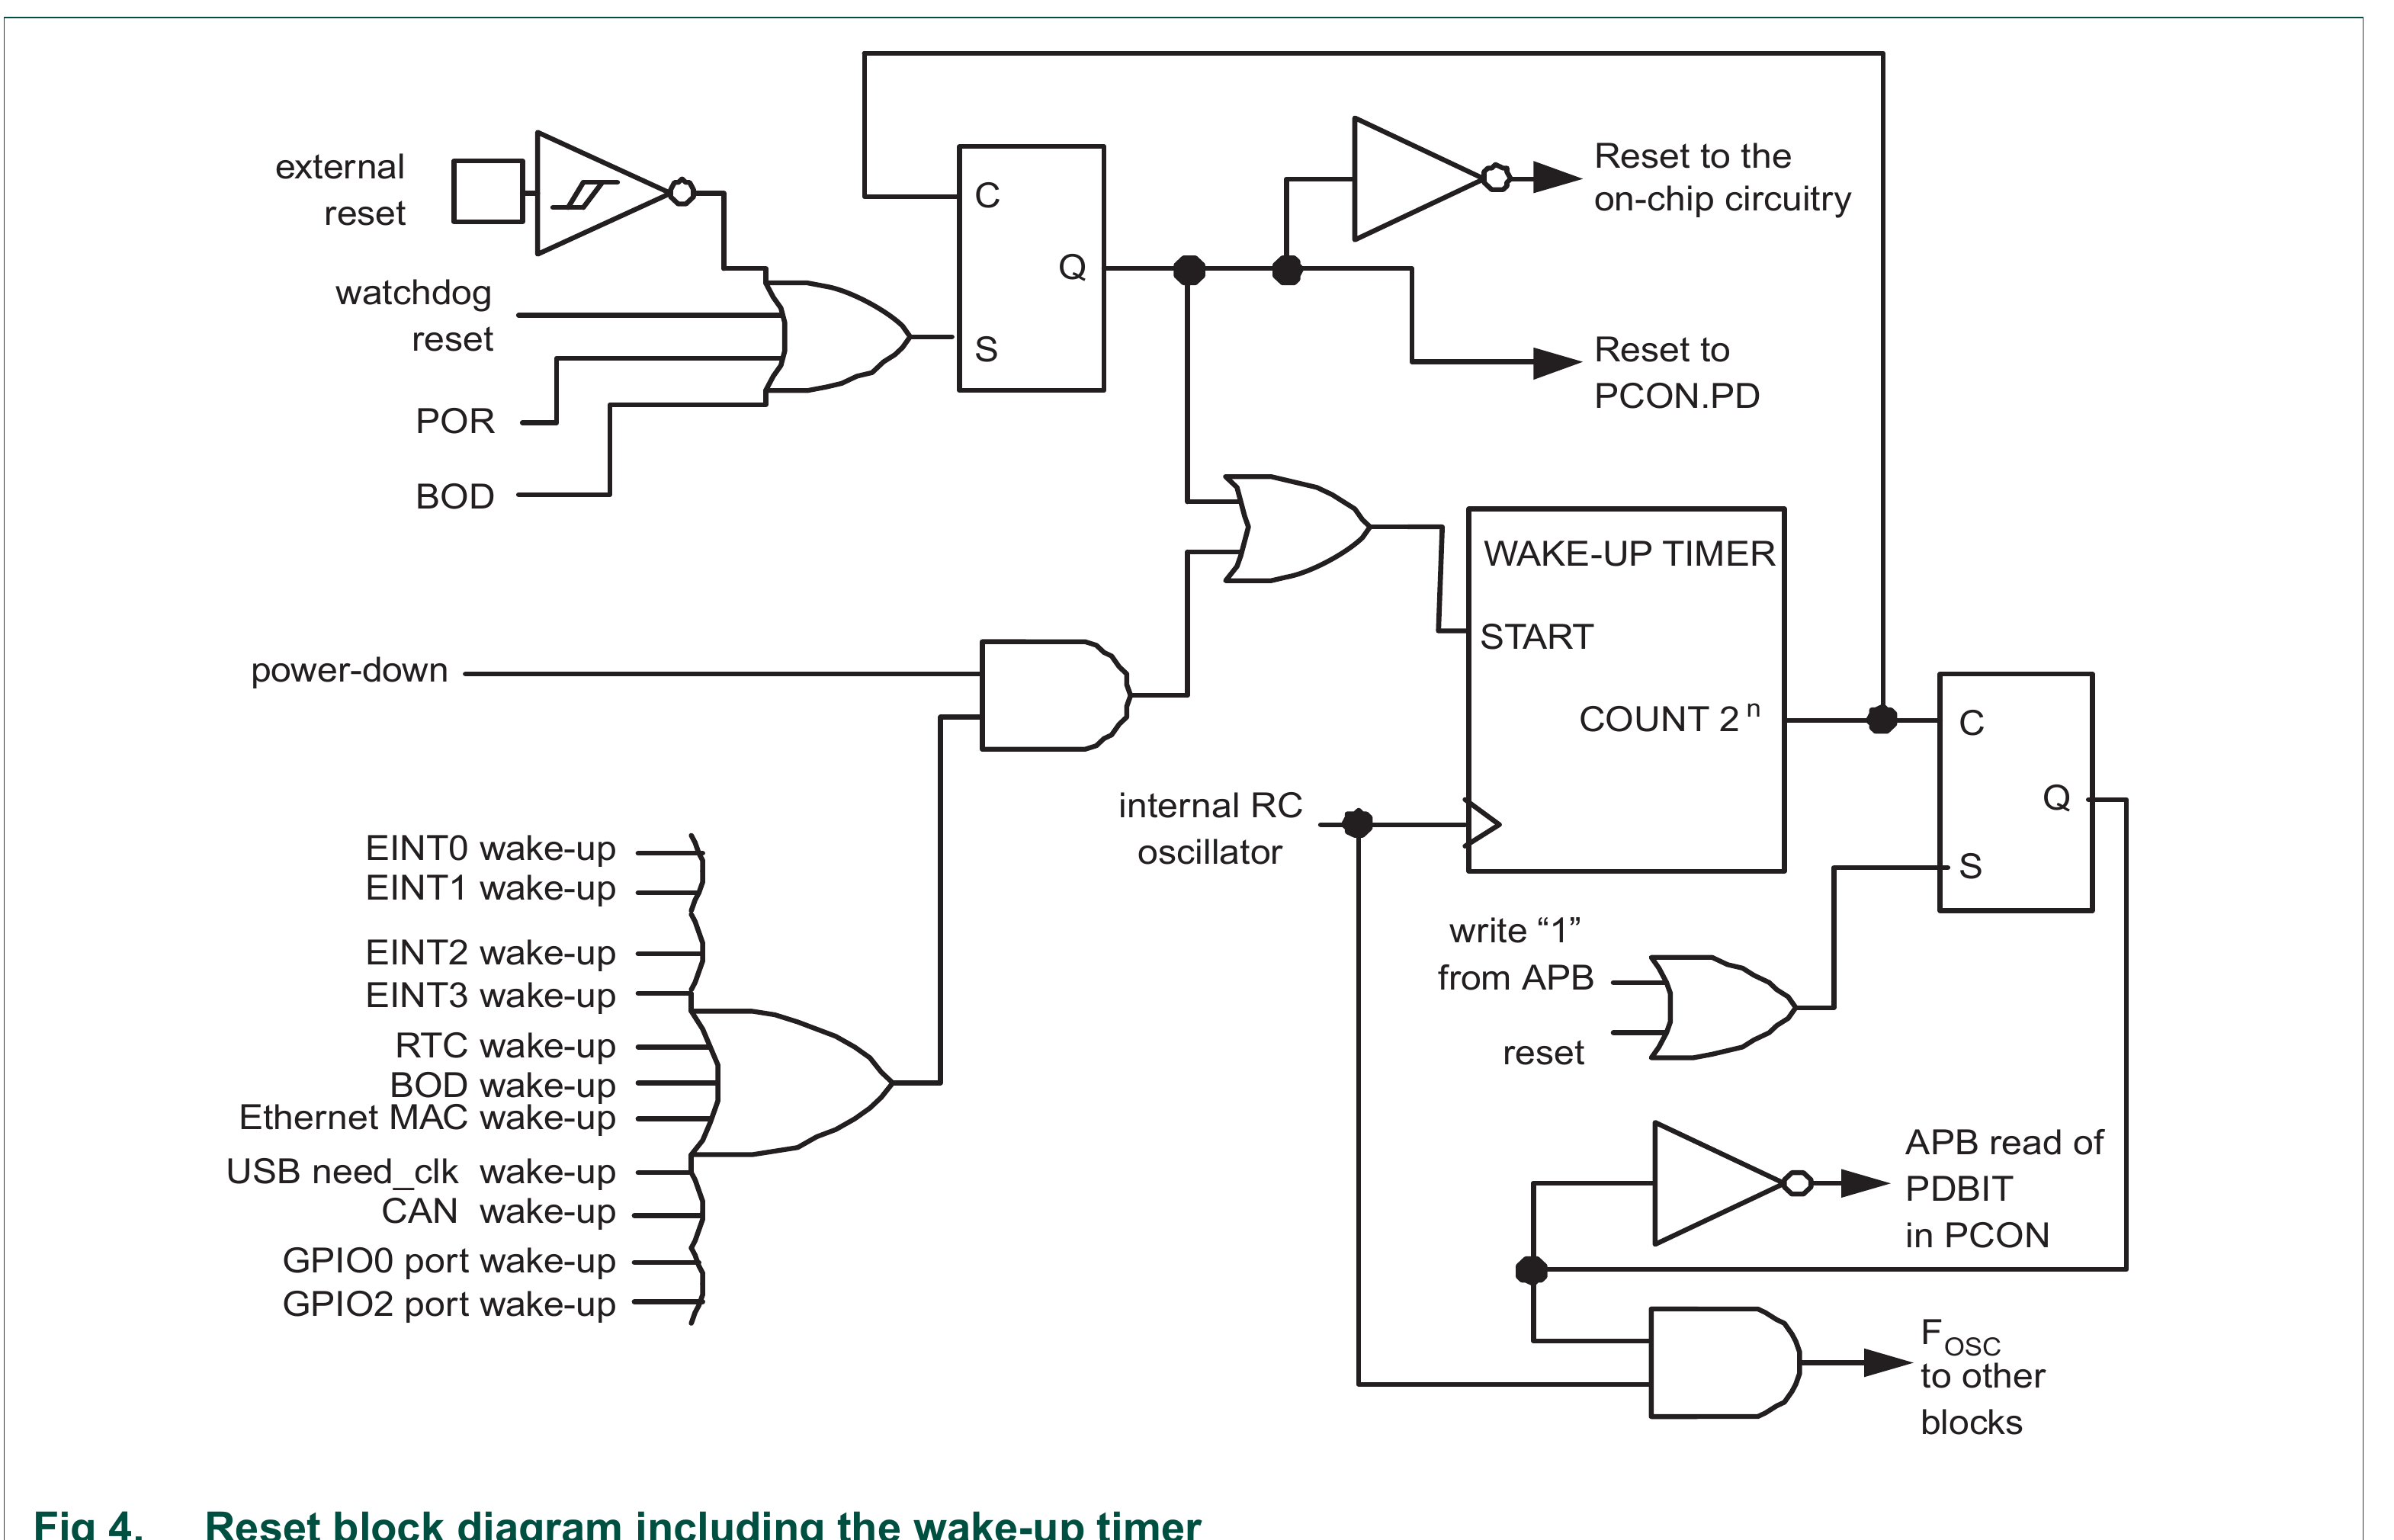
\includegraphics[width=0.96\textwidth]{images/system_control_reset_p19_fig4.png}
  \caption{L\'ogica de reset y \textit{wake-up timer} del bloque System control (Fig 4).}
\end{figure}

\paragraph{Secuencia pr\'actica de arranque}
\begin{enumerate}
  \item Sube la tensi\'on \texttt{VDD(REG)(3V3)} hasta superar el umbral v\'alido de operaci\'on.
  \item Ante una fuente de reset, el primer clock que arranca es el \textit{Internal RC Oscillator} (IRC), que es la fuente de clock por defecto despu\'es de encendido o reset.
  \item Cuando el IRC ya est\'a estable, la l\'ogica interna sincroniza la se\~nal de reset con ese clock.
  \item Desde la liberaci\'on sincronizada del reset corren en paralelo el \textit{IRC wake-up timer} y el temporizador de arranque de la flash.
  \item Cuando la flash ya est\'a lista para ser accedida, comienza la lectura desde memoria y se ejecuta el c\'odigo de arranque en ROM.
  \item Al terminar el \textit{boot code}, el procesador pasa a ejecutar el \textit{user code}. Reci\'en despu\'es, si el firmware lo decide, puede habilitar el oscilador principal y conmutar la fuente de clock en el cap\'itulo 4.
\end{enumerate}

\begin{table}[H]
  \centering
  \small
  \renewcommand{\arraystretch}{1.15}
  \caption{Reset Source Identification register \texttt{RSID} (Table 8)}
  \begin{tabularx}{0.96\textwidth}{|>{\centering\arraybackslash}p{0.08\textwidth}|>{\raggedright\arraybackslash}p{0.14\textwidth}|>{\raggedright\arraybackslash}X|>{\centering\arraybackslash}p{0.12\textwidth}|}
    \hline
    \textbf{Bit} & \textbf{S\'imbolo} & \textbf{Descripci\'on} & \textbf{Reset} \\
    \hline
    \texttt{0} & \texttt{POR} & Se activa con \textit{Power-On Reset}. Tiene prioridad fuerte: al activarse limpia los dem\'as bits, salvo que otra fuente siga presente despu\'es de liberarse el POR. & ver texto \\
    \hline
    \texttt{1} & \texttt{EXTR} & Indica reset por pin \texttt{RESET}. Solo se limpia por software o por POR. & ver texto \\
    \hline
    \texttt{2} & \texttt{WDTR} & Indica reset originado por \textit{Watchdog timeout} con \texttt{WDTRESET=1}. Solo se limpia por software o por POR. & ver texto \\
    \hline
    \texttt{3} & \texttt{BODR} & Indica que \texttt{VDD(REG)(3V3)} cay\'o por debajo del umbral de reset del BOD. Su interpretaci\'on depende de c\'omo cay\'o y se recuper\'o la alimentaci\'on. & ver texto \\
    \hline
    \texttt{31:4} & --- & Reservado. No escribir unos en bits reservados. & NA \\
    \hline
  \end{tabularx}
\end{table}

\paragraph{Nota t\'ecnica}
\texttt{RSID} conviene leerse al inicio del firmware, antes de limpiarlo, si se quiere registrar la causa del reinicio. En particular, \texttt{BODR} solo indica si \texttt{VDD(REG)(3V3)} cay\'o por debajo del umbral BOD cuando ocurre un reset con \texttt{POR=0}.

\subsection{Brown-out detection}
\begin{itemize}
  \item El \textbf{BOD} monitorea \texttt{VDD(REG)(3V3)} con dos umbrales.
  \item Primer nivel: genera una se\~nal hacia el NVIC cuando la tensi\'on cae por debajo del umbral de interrupci\'on (t\'ipicamente \texttt{2.2 V}); si esa interrupci\'on no est\'a habilitada, el evento puede vigilarse leyendo el \textit{Raw Interrupt Status Register}.
  \item Segundo nivel: fuerza reset cuando la tensi\'on cae por debajo del umbral de reset (t\'ipicamente \texttt{1.85 V}).
  \item El objetivo pr\'actico es evitar operaci\'on no confiable y proteger la flash frente a baja tensi\'on.
\end{itemize}

\paragraph{Nota t\'ecnica}
Un \textit{brown-out} transitorio puede sacar al dispositivo de \textit{Power-down} sin dejar un flag de wake-up tan evidente como otros eventos. Si no aparece otra causa latcheada, ese despertar puede atribuirse a BOD.

\subsection{Interrupciones externas \texttt{EINT0..3}}
\begin{itemize}
  \item Cada l\'inea \texttt{EINT} puede configurarse como sensible a \textbf{nivel} o \textbf{flanco}.
  \item En modo nivel, \texttt{EXTPOLAR} elige activo en alto o en bajo.
  \item En modo flanco, \texttt{EXTPOLAR} elige subida o bajada.
  \item Las interrupciones externas tambi\'en pueden actuar como fuente de wake-up desde \textit{Power-down}.
\end{itemize}

\begin{figure}[H]
  \centering
  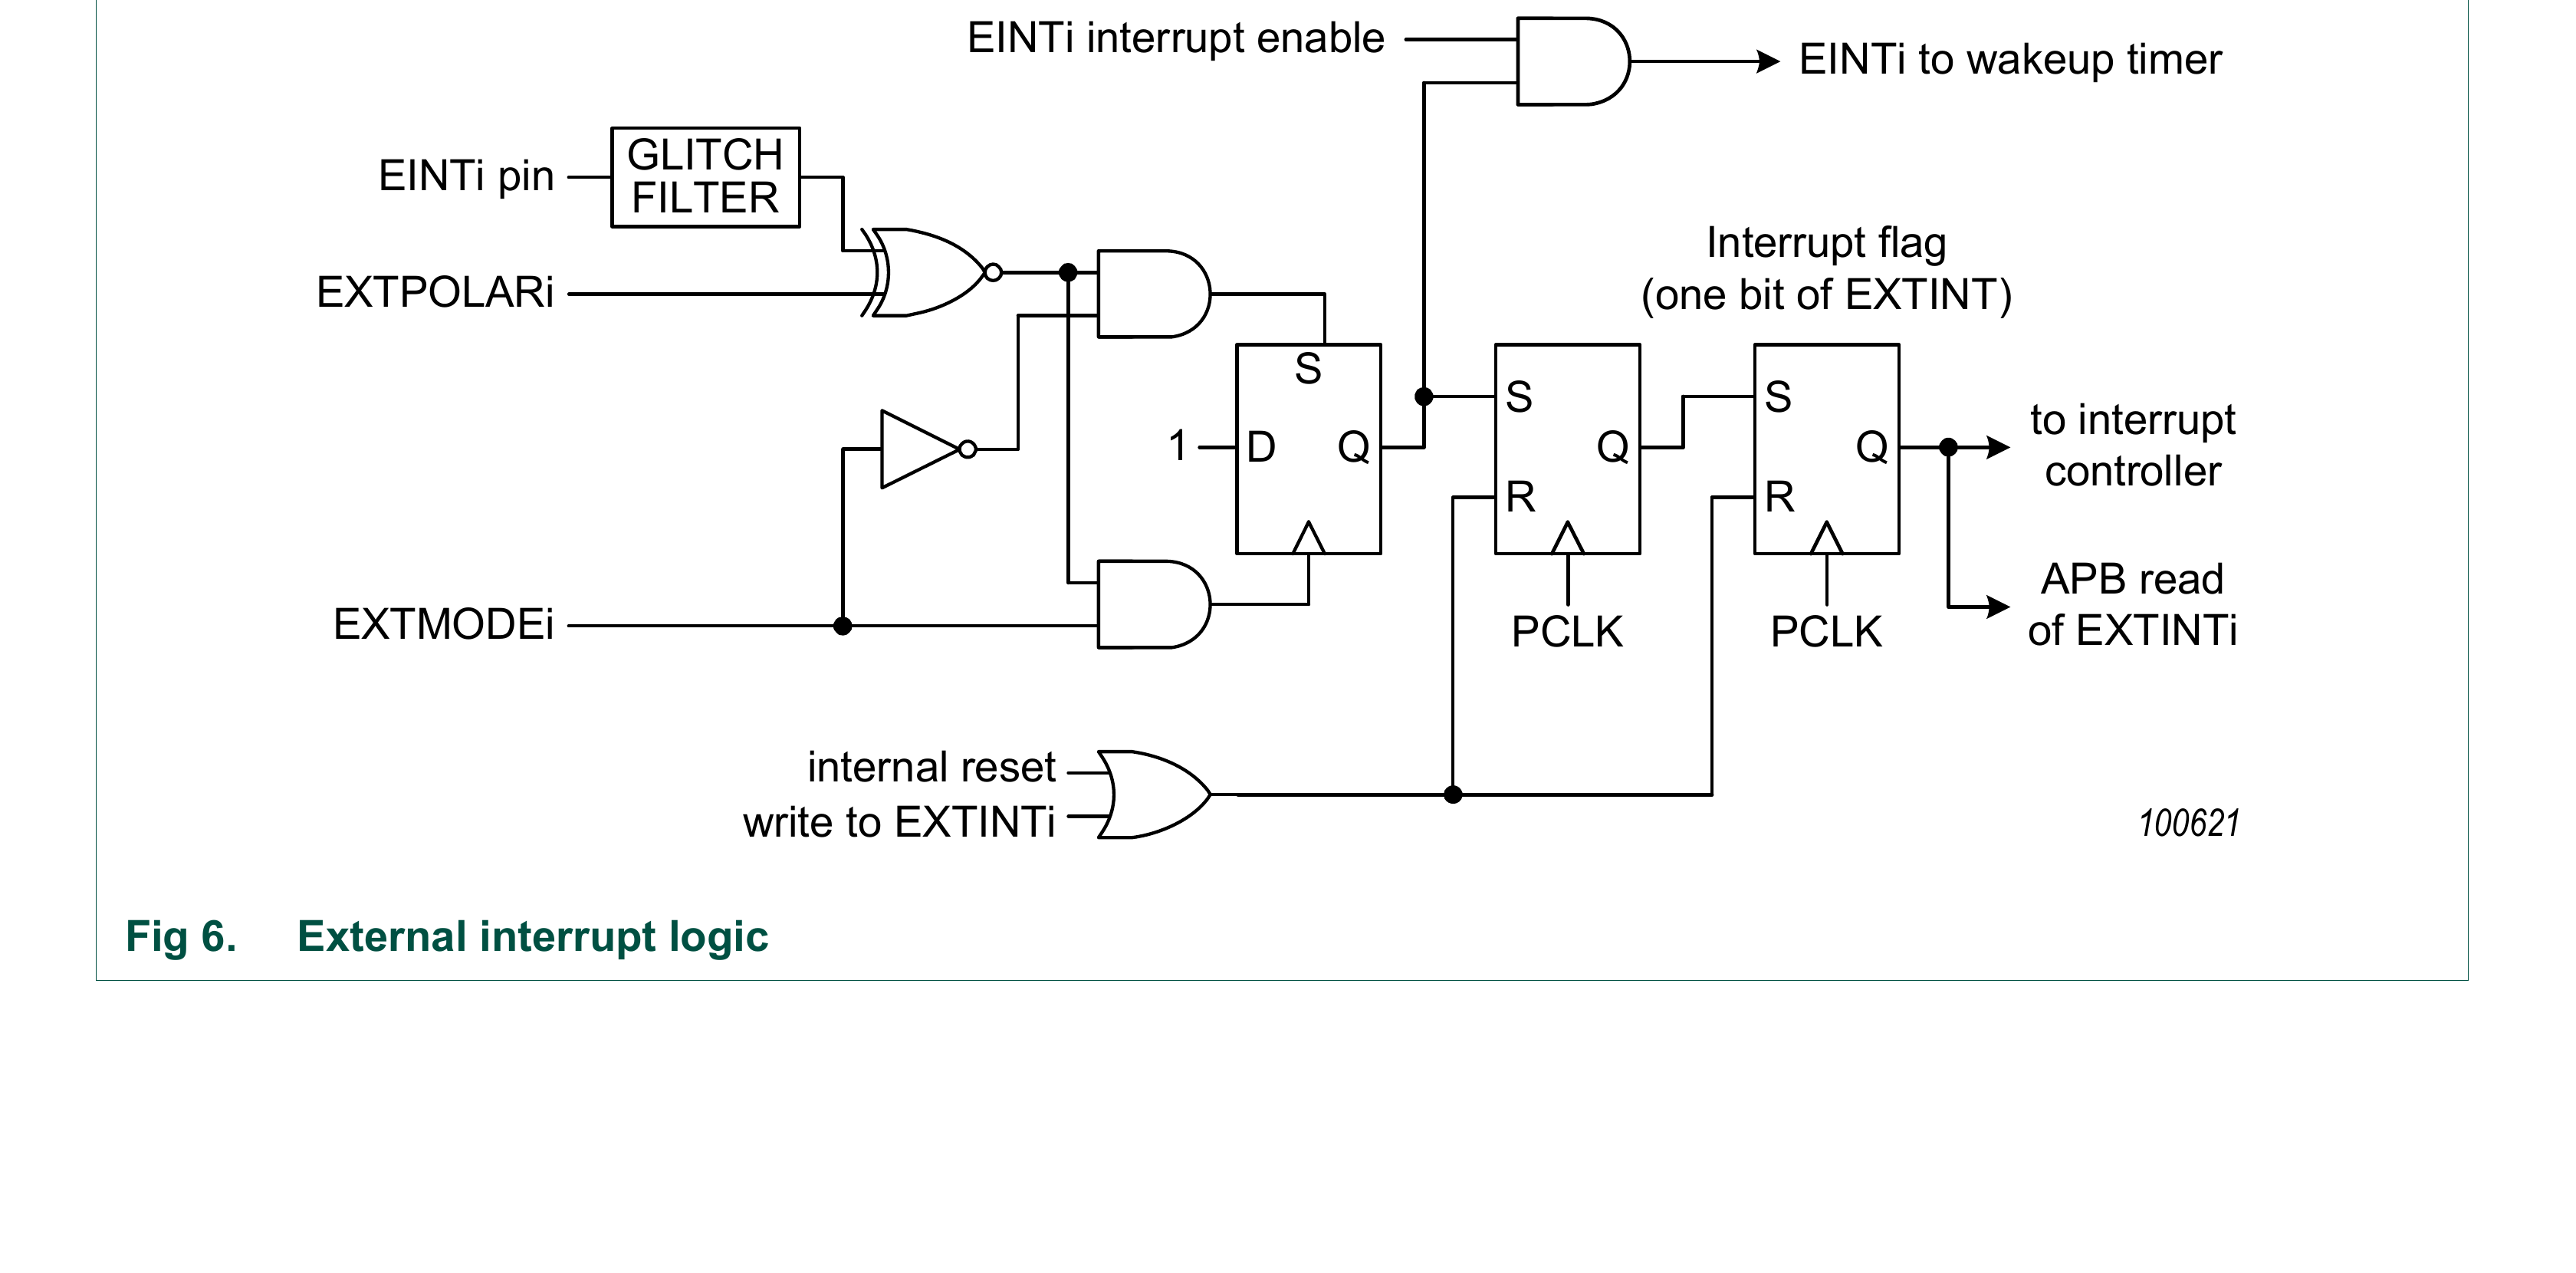
\includegraphics[width=0.96\textwidth]{images/system_control_eint_p23_fig6.png}
  \caption{L\'ogica interna de \texttt{EINTi} y relaci\'on con \texttt{EXTINT}, NVIC y wake-up (Fig 6).}
\end{figure}

\begin{table}[H]
  \centering
  \small
  \renewcommand{\arraystretch}{1.15}
  \caption{External interrupt registers (Table 9)}
  \begin{tabularx}{0.96\textwidth}{|>{\raggedright\arraybackslash}p{0.16\textwidth}|>{\raggedright\arraybackslash}X|>{\centering\arraybackslash}p{0.10\textwidth}|>{\centering\arraybackslash}p{0.10\textwidth}|>{\centering\arraybackslash}p{0.16\textwidth}|}
    \hline
    \textbf{Registro} & \textbf{Funci\'on} & \textbf{Acceso} & \textbf{Reset} & \textbf{Direcci\'on} \\
    \hline
    \texttt{EXTINT} & Flags de interrupci\'on para \texttt{EINT0..3}. & R/W & \texttt{0x00} & \texttt{0x400F C140} \\
    \hline
    \texttt{EXTMODE} & Selecciona sensibilidad por nivel o por flanco. & R/W & \texttt{0x00} & \texttt{0x400F C148} \\
    \hline
    \texttt{EXTPOLAR} & Selecciona nivel alto/bajo o flanco ascendente/descendente. & R/W & \texttt{0x00} & \texttt{0x400F C14C} \\
    \hline
  \end{tabularx}
\end{table}

\begin{table}[H]
  \centering
  \small
  \renewcommand{\arraystretch}{1.15}
  \caption{External Interrupt Flag register \texttt{EXTINT} (Table 10)}
  \begin{tabularx}{0.96\textwidth}{|>{\centering\arraybackslash}p{0.10\textwidth}|>{\raggedright\arraybackslash}p{0.14\textwidth}|>{\raggedright\arraybackslash}X|>{\centering\arraybackslash}p{0.10\textwidth}|}
    \hline
    \textbf{Bit} & \textbf{S\'imbolo} & \textbf{Descripci\'on} & \textbf{Reset} \\
    \hline
    \texttt{0} & \texttt{EINT0} & Flag de evento para \texttt{EINT0}. En modo nivel se mantiene activo mientras el pin permanezca en su estado activo. En modo flanco se activa cuando ocurre el flanco seleccionado. Se limpia escribiendo \texttt{1} en el bit, salvo que el pin siga activo en modo nivel. & \texttt{0} \\
    \hline
    \texttt{1} & \texttt{EINT1} & Igual que el bit anterior, aplicado a \texttt{EINT1}. & \texttt{0} \\
    \hline
    \texttt{2} & \texttt{EINT2} & Igual que el bit anterior, aplicado a \texttt{EINT2}. & \texttt{0} \\
    \hline
    \texttt{3} & \texttt{EINT3} & Igual que el bit anterior, aplicado a \texttt{EINT3}. & \texttt{0} \\
    \hline
    \texttt{31:4} & --- & Reservado. & NA \\
    \hline
  \end{tabularx}
\end{table}

\begin{table}[H]
  \centering
  \small
  \renewcommand{\arraystretch}{1.15}
  \caption{External Interrupt Mode register \texttt{EXTMODE} (Table 11)}
  \begin{tabularx}{0.96\textwidth}{|>{\centering\arraybackslash}p{0.10\textwidth}|>{\raggedright\arraybackslash}p{0.16\textwidth}|>{\raggedright\arraybackslash}X|>{\centering\arraybackslash}p{0.10\textwidth}|}
    \hline
    \textbf{Bit} & \textbf{S\'imbolo} & \textbf{Valor / Descripci\'on} & \textbf{Reset} \\
    \hline
    \texttt{0} & \texttt{EXTMODE0} & \texttt{0}: \texttt{EINT0} sensible a nivel. \texttt{1}: \texttt{EINT0} sensible a flanco. & \texttt{0} \\
    \hline
    \texttt{1} & \texttt{EXTMODE1} & \texttt{0}: \texttt{EINT1} sensible a nivel. \texttt{1}: \texttt{EINT1} sensible a flanco. & \texttt{0} \\
    \hline
    \texttt{2} & \texttt{EXTMODE2} & \texttt{0}: \texttt{EINT2} sensible a nivel. \texttt{1}: \texttt{EINT2} sensible a flanco. & \texttt{0} \\
    \hline
    \texttt{3} & \texttt{EXTMODE3} & \texttt{0}: \texttt{EINT3} sensible a nivel. \texttt{1}: \texttt{EINT3} sensible a flanco. & \texttt{0} \\
    \hline
    \texttt{31:4} & --- & Reservado. & NA \\
    \hline
  \end{tabularx}
\end{table}

\begin{table}[H]
  \centering
  \small
  \renewcommand{\arraystretch}{1.15}
  \caption{External Interrupt Polarity register \texttt{EXTPOLAR} (Table 12)}
  \begin{tabularx}{0.96\textwidth}{|>{\centering\arraybackslash}p{0.10\textwidth}|>{\raggedright\arraybackslash}p{0.16\textwidth}|>{\raggedright\arraybackslash}X|>{\centering\arraybackslash}p{0.10\textwidth}|}
    \hline
    \textbf{Bit} & \textbf{S\'imbolo} & \textbf{Valor / Descripci\'on} & \textbf{Reset} \\
    \hline
    \texttt{0} & \texttt{EXTPOLAR0} & \texttt{0}: \texttt{EINT0} activo en bajo o por flanco descendente. \texttt{1}: \texttt{EINT0} activo en alto o por flanco ascendente. & \texttt{0} \\
    \hline
    \texttt{1} & \texttt{EXTPOLAR1} & \texttt{0}: \texttt{EINT1} activo en bajo o por flanco descendente. \texttt{1}: \texttt{EINT1} activo en alto o por flanco ascendente. & \texttt{0} \\
    \hline
    \texttt{2} & \texttt{EXTPOLAR2} & \texttt{0}: \texttt{EINT2} activo en bajo o por flanco descendente. \texttt{1}: \texttt{EINT2} activo en alto o por flanco ascendente. & \texttt{0} \\
    \hline
    \texttt{3} & \texttt{EXTPOLAR3} & \texttt{0}: \texttt{EINT3} activo en bajo o por flanco descendente. \texttt{1}: \texttt{EINT3} activo en alto o por flanco ascendente. & \texttt{0} \\
    \hline
    \texttt{31:4} & --- & Reservado. & NA \\
    \hline
  \end{tabularx}
\end{table}

\paragraph{Nota t\'ecnica}
Cuando se cambia \texttt{EXTMODE} o \texttt{EXTPOLAR}, el datasheet indica deshabilitar antes la interrupci\'on en el NVIC y escribir \texttt{1} en el bit correspondiente de \texttt{EXTINT} antes de volver a habilitarla. Si no se hace, pueden aparecer interrupciones espurias o fallas al reingresar a \textit{Power-down}.

\subsection{System Controls and Status register}
\begin{itemize}
  \item \texttt{SCS} agrupa bits de control y estado del oscilador principal.
  \item Como el LPC17xx arranca siempre con el \textit{Internal RC Oscillator}, el oscilador principal solo se inicia por pedido expl\'icito de software.
  \item Antes de usarlo como fuente de clock debe seleccionarse el rango de frecuencia y esperarse a que \texttt{OSCSTAT} indique estabilidad.
  \item \texttt{OSCEN=1} solo produce el arranque real del oscilador si la circuiter\'ia externa correcta est\'a conectada a \texttt{XTAL1} y \texttt{XTAL2}.
\end{itemize}

\begin{table}[H]
  \centering
  \small
  \renewcommand{\arraystretch}{1.15}
  \caption{System Controls and Status register \texttt{SCS} (Table 13)}
  \begin{tabularx}{0.96\textwidth}{|>{\centering\arraybackslash}p{0.10\textwidth}|>{\raggedright\arraybackslash}p{0.16\textwidth}|>{\raggedright\arraybackslash}X|>{\centering\arraybackslash}p{0.11\textwidth}|>{\centering\arraybackslash}p{0.10\textwidth}|}
    \hline
    \textbf{Bit} & \textbf{S\'imbolo} & \textbf{Valor / Descripci\'on} & \textbf{Acceso} & \textbf{Reset} \\
    \hline
    \texttt{3:0} & --- & Reservado. & NA & NA \\
    \hline
    \texttt{4} & \texttt{OSCRANGE} & \texttt{0}: rango de \texttt{1 MHz} a \texttt{20 MHz}. \texttt{1}: rango de \texttt{15 MHz} a \texttt{25 MHz}. & R/W & \texttt{0} \\
    \hline
    \texttt{5} & \texttt{OSCEN} & \texttt{0}: oscilador principal deshabilitado. \texttt{1}: oscilador principal habilitado. & R/W & \texttt{0} \\
    \hline
    \texttt{6} & \texttt{OSCSTAT} & \texttt{0}: el oscilador principal todav\'ia no est\'a listo. \texttt{1}: el oscilador principal est\'a estable y listo para usarse. & RO & \texttt{0} \\
    \hline
    \texttt{31:7} & --- & Reservado. & NA & NA \\
    \hline
  \end{tabularx}
\end{table}

\paragraph{Uso pr\'actico}
La secuencia t\'ipica es: configurar \texttt{OSCRANGE}, habilitar \texttt{OSCEN}, esperar \texttt{OSCSTAT=1} y reci\'en despu\'es conmutar la fuente de clock en el cap\'itulo 4.
}{}
\IfFileExists{chapter6.tex}{\setcounter{section}{5}
\section{LPC17xx Nested Vectored Interrupt Controller (NVIC)}

\subsection{Resumen del bloque}
\begin{itemize}
  \item El \texttt{NVIC} es parte integral del n\'ucleo ARM Cortex-M3 y centraliza la atenci\'on de excepciones del sistema e interrupciones de perif\'ericos.
  \item En el LPC17xx soporta \textbf{35 interrupciones vectorizadas}, \textbf{32 niveles de prioridad programables}, \textbf{tabla vectorial reubicable}, \textbf{NMI} y \textbf{disparo de IRQ por software}.
  \item Los registros clave del bloque son \texttt{ISER0/1}, \texttt{ICER0/1}, \texttt{ISPR0/1}, \texttt{ICPR0/1}, \texttt{IABR0/1}, \texttt{IPR0..8} y \texttt{STIR}.
\end{itemize}

\paragraph{Nota t\'ecnica}
En jerarqu\'ia conceptual, \textbf{Reset} queda por encima de todo, luego \textbf{NMI}, luego \textbf{HardFault} y despu\'es el resto de excepciones configurables e \texttt{IRQ} normales. \texttt{IRQ} significa \textit{Interrupt Request}: una solicitud de interrupci\'on perif\'erica ordinaria manejada por el \texttt{NVIC}. \texttt{NMI} es una excepci\'on especial no enmascarable, no una \texttt{IRQ} perif\'erica com\'un.

\subsection{C\'omo leer este cap\'itulo}
\begin{itemize}
  \item \textbf{Interrupt ID:} n\'umero l\'ogico de la \texttt{IRQ} perif\'erica dentro del \texttt{NVIC}.
  \item \textbf{Exception Number:} posici\'on de esa \texttt{IRQ} dentro de la tabla completa de excepciones del Cortex-M3. Para las \texttt{IRQ} externas del LPC17xx, empieza en \texttt{16}.
  \item \textbf{Vector Offset:} desplazamiento en bytes de la entrada dentro de la tabla vectorial. En pr\'actica, \texttt{Vector Offset = Exception Number * 4}.
  \item La tabla vectorial no guarda el c\'odigo del handler sino la \textbf{direcci\'on} de entrada del handler. Cuando una excepci\'on o \texttt{IRQ} es aceptada, el n\'ucleo lee esa direcci\'on y salta a ella.
\end{itemize}

\paragraph{Estados de una interrupci\'on}
\begin{itemize}
  \item \textbf{enabled:} la l\'inea est\'a habilitada para ser atendida por el \texttt{NVIC}.
  \item \textbf{pending:} existe una solicitud de atenci\'on esperando turno.
  \item \textbf{active:} la interrupci\'on ya fue aceptada por el n\'ucleo y su \texttt{ISR} est\'a siendo atendida o forma parte del contexto activo anidado.
\end{itemize}

\paragraph{Nota t\'ecnica}
En flujo normal, el firmware suele habilitar la \texttt{IRQ} y limpiar la \textbf{causa real} en el perif\'erico dentro de la \texttt{ISR}. El estado \texttt{active} lo maneja autom\'aticamente el Cortex-M3/\texttt{NVIC}. El estado \texttt{pending} puede originarse por hardware o forzarse por software con \texttt{ISPR}. Si una \texttt{ISR} de mayor prioridad preempta a otra, la primera no ``vuelve'' a \texttt{pending}: queda suspendida y luego se retoma.

\subsection{Fuentes de interrupci\'on}
\scriptsize
\renewcommand{\arraystretch}{1.12}
\setlength{\LTleft}{0pt}
\setlength{\LTright}{0pt}

\begin{longtable}{|>{\centering\arraybackslash}p{0.07\textwidth}|>{\centering\arraybackslash}p{0.10\textwidth}|>{\centering\arraybackslash}p{0.12\textwidth}|>{\raggedright\arraybackslash}p{0.19\textwidth}|>{\raggedright\arraybackslash}p{0.40\textwidth}|}
\caption{Conexi\'on de fuentes de interrupci\'on al Vectored Interrupt Controller (Table 50)} \\
\hline
\textbf{Interrupt ID} & \textbf{Exception Number} & \textbf{Vector Offset} & \textbf{Funci\'on} & \textbf{Flag(s)} \\
\hline
\endfirsthead
\hline
\textbf{Interrupt ID} & \textbf{Exception Number} & \textbf{Vector Offset} & \textbf{Funci\'on} & \textbf{Flag(s)} \\
\hline
\endhead
0 & 16 & \texttt{0x40} & \texttt{WDT} & Interrupci\'on de watchdog (\texttt{WDINT}). \\
\hline
1 & 17 & \texttt{0x44} & \texttt{Timer 0} & Match 0--1 (\texttt{MR0}, \texttt{MR1}). \\
\hline
2 & 18 & \texttt{0x48} & \texttt{Timer 1} & Match 0--2 (\texttt{MR0}, \texttt{MR1}, \texttt{MR2}); Capture 0--1 (\texttt{CR0}, \texttt{CR1}). \\
\hline
3 & 19 & \texttt{0x4C} & \texttt{Timer 2} & Match 0--3; Capture 0--1. \\
\hline
4 & 20 & \texttt{0x50} & \texttt{Timer 3} & Match 0--3; Capture 0--1. \\
\hline
5 & 21 & \texttt{0x54} & \texttt{UART0} & \texttt{RLS}, \texttt{THRE}, \texttt{RDA}, \texttt{CTI}, \texttt{ABEO}, \texttt{ABTO}. \\
\hline
6 & 22 & \texttt{0x58} & \texttt{UART1} & \texttt{RLS}, \texttt{THRE}, \texttt{RDA}, \texttt{CTI}, cambio de control de m\'odem, \texttt{ABEO}, \texttt{ABTO}. \\
\hline
7 & 23 & \texttt{0x5C} & \texttt{UART2} & \texttt{RLS}, \texttt{THRE}, \texttt{RDA}, \texttt{CTI}, \texttt{ABEO}, \texttt{ABTO}. \\
\hline
8 & 24 & \texttt{0x60} & \texttt{UART3} & \texttt{RLS}, \texttt{THRE}, \texttt{RDA}, \texttt{CTI}, \texttt{ABEO}, \texttt{ABTO}. \\
\hline
9 & 25 & \texttt{0x64} & \texttt{PWM1} & Match 0--6 de \texttt{PWM1}; Capture 0--1 de \texttt{PWM1}. \\
\hline
10 & 26 & \texttt{0x68} & \texttt{I2C0} & \texttt{SI} (cambio de estado). \\
\hline
11 & 27 & \texttt{0x6C} & \texttt{I2C1} & \texttt{SI} (cambio de estado). \\
\hline
12 & 28 & \texttt{0x70} & \texttt{I2C2} & \texttt{SI} (cambio de estado). \\
\hline
13 & 29 & \texttt{0x74} & \texttt{SPI} & \texttt{SPIF} (flag de interrupci\'on SPI), \texttt{MODF} (modo fault). \\
\hline
14 & 30 & \texttt{0x78} & \texttt{SSP0} & \texttt{Tx FIFO half empty}, \texttt{Rx FIFO half full}, \texttt{Rx Timeout}, \texttt{Rx Overrun}. \\
\hline
15 & 31 & \texttt{0x7C} & \texttt{SSP1} & \texttt{Tx FIFO half empty}, \texttt{Rx FIFO half full}, \texttt{Rx Timeout}, \texttt{Rx Overrun}. \\
\hline
16 & 32 & \texttt{0x80} & \texttt{PLL0 (Main PLL)} & Lock de \texttt{PLL0} (\texttt{PLOCK0}). \\
\hline
17 & 33 & \texttt{0x84} & \texttt{RTC} & Incremento de contador (\texttt{RTCCIF}). \\
\hline
18 & 34 & \texttt{0x88} & \texttt{External Interrupt} & Interrupci\'on externa 0 (\texttt{EINT0}). \\
\hline
19 & 35 & \texttt{0x8C} & \texttt{External Interrupt} & Interrupci\'on externa 1 (\texttt{EINT1}). \\
\hline
20 & 36 & \texttt{0x90} & \texttt{External Interrupt} & Interrupci\'on externa 2 (\texttt{EINT2}). \\
\hline
21 & 37 & \texttt{0x94} & \texttt{External Interrupt} & \texttt{RTCALF} e interrupci\'on externa 3 (\texttt{EINT3}). Nota: \texttt{EINT3} comparte canal con interrupciones GPIO. \\
\hline
22 & 38 & \texttt{0x98} & \texttt{ADC} & Fin de conversi\'on del convertidor A/D. \\
\hline
23 & 39 & \texttt{0x9C} & \texttt{BOD} & Detecci\'on de \textit{brown-out}. \\
\hline
24 & 40 & \texttt{0xA0} & \texttt{USB} & \texttt{USB\_INT\_REQ\_LP}, \texttt{USB\_INT\_REQ\_HP}, \texttt{USB\_INT\_REQ\_DMA}. \\
\hline
25 & 41 & \texttt{0xA4} & \texttt{CAN} & \texttt{CAN Common}, \texttt{CAN0 Tx}, \texttt{CAN0 Rx}, \texttt{CAN1 Tx}, \texttt{CAN1 Rx}. \\
\hline
26 & 42 & \texttt{0xA8} & \texttt{GPDMA} & \texttt{IntStatus} de canal DMA 0, \texttt{IntStatus} de canal DMA 1, \texttt{irq}, \texttt{dmareq1}, \texttt{dmareq2}. \\
\hline
27 & 43 & \texttt{0xAC} & \texttt{I2S} & Interrupci\'on del bloque \texttt{I2S}. \\
\hline
28 & 44 & \texttt{0xB0} & \texttt{Ethernet} & \texttt{WakeupInt}, \texttt{SoftInt}, \texttt{TxDoneInt}, \texttt{TxFinishedInt}, \texttt{TxErrorInt}, \texttt{TxUnderrunInt}, \texttt{RxDoneInt}, \texttt{RxFinishedInt}, \texttt{RxErrorInt}, \texttt{RxOverrunInt}. \\
\hline
29 & 45 & \texttt{0xB4} & \texttt{Repetitive Interrupt Timer} & \texttt{RITINT}. \\
\hline
30 & 46 & \texttt{0xB8} & \texttt{Motor Control PWM} & \texttt{IPER[2:0]}, \texttt{IPW[2:0]}, \texttt{ICAP[2:0]}, \texttt{FES}. \\
\hline
31 & 47 & \texttt{0xBC} & \texttt{Quadrature Encoder} & \texttt{INX\_Int}, \texttt{TIM\_Int}, \texttt{VELC\_Int}, \texttt{DIR\_Int}, \texttt{ERR\_Int}, \texttt{ENCLK\_Int}, \texttt{POS0\_Int}, \texttt{POS1\_Int}, \texttt{POS2\_Int}, \texttt{REV\_Int}, \texttt{POS0REV\_Int}, \texttt{POS1REV\_Int}, \texttt{POS2REV\_Int}. \\
\hline
32 & 48 & \texttt{0xC0} & \texttt{PLL1 (USB PLL)} & Lock de \texttt{PLL1} (\texttt{PLOCK1}). \\
\hline
33 & 49 & \texttt{0xC4} & \texttt{USB Activity Interrupt} & \texttt{USB\_NEED\_CLK}. \\
\hline
34 & 50 & \texttt{0xC8} & \texttt{CAN Activity Interrupt} & \texttt{CAN1WAKE}, \texttt{CAN2WAKE}. \\
\hline
\end{longtable}
\normalsize

\paragraph{Nota t\'ecnica}
La \texttt{Table 50} no enumera \texttt{NMI} como una \texttt{IRQ} perif\'erica normal porque \texttt{NMI} es una excepci\'on especial del Cortex-M3. Si se usa desde se\~nal externa, debe conectarse la funci\'on \texttt{NMI} al pin \texttt{P2.10 / EINT0n / NMI}; con esa funci\'on activa, un nivel l\'ogico alto en el pin dispara la \texttt{NMI}.

\subsection{Remapeo de tabla vectorial}
\begin{itemize}
  \item El Cortex-M3 permite reubicar la tabla de vectores en otra direcci\'on del mapa de memoria mediante \texttt{VTOR} (\textit{Vector Table Offset Register}).
  \item La tabla puede ubicarse en el primer \textbf{1 GB} del espacio de direcciones del Cortex-M3.
  \item En la familia LPC17xx debe alinearse a \textbf{256 palabras} (\textbf{1024 bytes}).
  \item Desde el punto de vista pr\'actico, \texttt{VTOR} define la \textbf{base} desde la cual el n\'ucleo lee las direcciones de handlers.
\end{itemize}

\paragraph{Nota t\'ecnica}
La tabla vectorial no contiene el c\'odigo del handler sino la \textbf{direcci\'on} de entrada del handler. Si el firmware mueve \texttt{VTOR}, la nueva tabla debe existir realmente en esa memoria y tener entradas v\'alidas; de lo contrario, el n\'ucleo saltar\'a a direcciones err\'oneas cuando ocurra una excepci\'on o una \texttt{IRQ}.

\paragraph{Uso pr\'actico}
Los usos m\'as comunes de \texttt{VTOR} son \textbf{bootloaders}, esquemas con \textbf{tabla vectorial en SRAM} y configuraciones donde el flujo de arranque necesita cambiar qu\'e imagen de firmware atiende las interrupciones.

\begin{table}[H]
  \centering
  \small
  \renewcommand{\arraystretch}{1.15}
  \caption{Ejemplos de remapeo de tabla vectorial a partir de \texttt{VTOR}}
  \begin{tabularx}{0.96\textwidth}{|>{\raggedright\arraybackslash}p{0.18\textwidth}|>{\raggedright\arraybackslash}p{0.22\textwidth}|>{\raggedright\arraybackslash}X|}
    \hline
    \textbf{Ubicaci\'on} & \textbf{Valor en \texttt{VTOR}} & \textbf{Interpretaci\'on} \\
    \hline
    SRAM local & \texttt{0x1000 0000} & La tabla queda al comienzo de la SRAM local. El bit 29 vale \texttt{0}; en la explicaci\'on de ARM esto cae en ``code space'', aunque en la pr\'actica conviene pensarlo como parte de la direcci\'on. \\
    \hline
    AHB SRAM & \texttt{0x2007 C000} & La tabla queda al comienzo de la AHB SRAM. El bit 29 vale \texttt{1}; ARM lo describe como ``SRAM space'', pero para firmware conviene tratarlo simplemente como base de direcci\'on. \\
    \hline
  \end{tabularx}
\end{table}

\subsection{Mapa de registros}
\scriptsize
\renewcommand{\arraystretch}{1.12}
\begin{longtable}{|>{\raggedright\arraybackslash}p{0.16\textwidth}|>{\raggedright\arraybackslash}p{0.36\textwidth}|>{\centering\arraybackslash}p{0.09\textwidth}|>{\centering\arraybackslash}p{0.09\textwidth}|>{\raggedright\arraybackslash}p{0.18\textwidth}|}
\caption{Mapa de registros del NVIC (Table 51)} \\
\hline
\textbf{Name} & \textbf{Description} & \textbf{Access} & \textbf{Reset} & \textbf{Address} \\
\hline
\endfirsthead
\hline
\textbf{Name} & \textbf{Description} & \textbf{Access} & \textbf{Reset} & \textbf{Address} \\
\hline
\endhead
\texttt{ISER0} a \texttt{ISER1} & Registros de \textit{Interrupt Set-Enable}. Permiten habilitar interrupciones y leer el estado de habilitaci\'on de funciones perif\'ericas espec\'ificas. & R/W & 0 & \texttt{ISER0 - 0xE000 E100}; \texttt{ISER1 - 0xE000 E104}. \\
\hline
\texttt{ICER0} a \texttt{ICER1} & Registros de \textit{Interrupt Clear-Enable}. Permiten deshabilitar interrupciones y leer el estado de habilitaci\'on de funciones perif\'ericas espec\'ificas. & R/W & 0 & \texttt{ICER0 - 0xE000 E180}; \texttt{ICER1 - 0xE000 E184}. \\
\hline
\texttt{ISPR0} a \texttt{ISPR1} & Registros de \textit{Interrupt Set-Pending}. Permiten cambiar el estado de la interrupci\'on a \texttt{pending} y leer el estado de pendiente para funciones perif\'ericas espec\'ificas. & R/W & 0 & \texttt{ISPR0 - 0xE000 E200}; \texttt{ISPR1 - 0xE000 E204}. \\
\hline
\texttt{ICPR0} a \texttt{ICPR1} & Registros de \textit{Interrupt Clear-Pending}. Permiten cambiar el estado de la interrupci\'on a ``not pending'' y leer el estado de pendiente para funciones perif\'ericas espec\'ificas. & R/W & 0 & \texttt{ICPR0 - 0xE000 E280}; \texttt{ICPR1 - 0xE000 E284}. \\
\hline
\texttt{IABR0} a \texttt{IABR1} & Registros de \textit{Interrupt Active Bit}. Permiten leer el estado activo actual para funciones perif\'ericas espec\'ificas. & RO & 0 & \texttt{IABR0 - 0xE000 E300}; \texttt{IABR1 - 0xE000 E304}. \\
\hline
\texttt{IPR0} a \texttt{IPR8} & Registros de prioridad. Permiten asignar una prioridad a cada interrupci\'on; cada registro contiene campos de prioridad de 5 bits para 4 interrupciones. & R/W & 0 & \texttt{IPR0 - 0xE000 E400} a \texttt{IPR8 - 0xE000 E420}. \\
\hline
\texttt{STIR} & \textit{Software Trigger Interrupt Register}. Permite que software genere una interrupci\'on. & WO & 0 & \texttt{STIR - 0xE000 EF00}. \\
\hline
\end{longtable}
\normalsize

\subsection{\texttt{ISER0} y \texttt{ISER1}}
Los registros \texttt{ISER} controlan el estado \texttt{enabled}. Escribir \texttt{1} en un bit habilita la \texttt{IRQ}; escribir \texttt{0} no produce efecto. La lectura devuelve si la interrupci\'on est\'a o no habilitada.

\begin{table}[H]
  \centering
  \small
  \renewcommand{\arraystretch}{1.12}
  \caption{Interrupt Set-Enable Register 0 register (\texttt{ISER0} - \texttt{0xE000 E100}) (Table 52)}
  \begin{tabularx}{0.96\textwidth}{|>{\centering\arraybackslash}p{0.08\textwidth}|>{\raggedright\arraybackslash}p{0.18\textwidth}|>{\raggedright\arraybackslash}X|}
    \hline
    \textbf{Bit} & \textbf{Name} & \textbf{Function} \\
    \hline
    0 & \texttt{ISE\_WDT} & Habilitaci\'on de interrupci\'on del Watchdog. Escritura: \texttt{0} no cambia nada, \texttt{1} habilita la interrupci\'on. Lectura: \texttt{0} indica deshabilitada, \texttt{1} indica habilitada. \\
    \hline
    1 & \texttt{ISE\_TIMER0} & Habilitaci\'on de interrupci\'on de Timer 0. Ver descripci\'on funcional del bit 0. \\
    \hline
    2 & \texttt{ISE\_TIMER1} & Habilitaci\'on de interrupci\'on de Timer 1. Ver bit 0. \\
    \hline
    3 & \texttt{ISE\_TIMER2} & Habilitaci\'on de interrupci\'on de Timer 2. Ver bit 0. \\
    \hline
    4 & \texttt{ISE\_TIMER3} & Habilitaci\'on de interrupci\'on de Timer 3. Ver bit 0. \\
    \hline
    5 & \texttt{ISE\_UART0} & Habilitaci\'on de interrupci\'on de UART0. Ver bit 0. \\
    \hline
    6 & \texttt{ISE\_UART1} & Habilitaci\'on de interrupci\'on de UART1. Ver bit 0. \\
    \hline
    7 & \texttt{ISE\_UART2} & Habilitaci\'on de interrupci\'on de UART2. Ver bit 0. \\
    \hline
    8 & \texttt{ISE\_UART3} & Habilitaci\'on de interrupci\'on de UART3. Ver bit 0. \\
    \hline
    9 & \texttt{ISE\_PWM} & Habilitaci\'on de interrupci\'on de PWM1. Ver bit 0. \\
    \hline
    10 & \texttt{ISE\_I2C0} & Habilitaci\'on de interrupci\'on de I2C0. Ver bit 0. \\
    \hline
    11 & \texttt{ISE\_I2C1} & Habilitaci\'on de interrupci\'on de I2C1. Ver bit 0. \\
    \hline
    12 & \texttt{ISE\_I2C2} & Habilitaci\'on de interrupci\'on de I2C2. Ver bit 0. \\
    \hline
    13 & \texttt{ISE\_SPI} & Habilitaci\'on de interrupci\'on de SPI. Ver bit 0. \\
    \hline
    14 & \texttt{ISE\_SSP0} & Habilitaci\'on de interrupci\'on de SSP0. Ver bit 0. \\
    \hline
    15 & \texttt{ISE\_SSP1} & Habilitaci\'on de interrupci\'on de SSP1. Ver bit 0. \\
    \hline
    16 & \texttt{ISE\_PLL0} & Habilitaci\'on de interrupci\'on de PLL0. Ver bit 0. \\
    \hline
    17 & \texttt{ISE\_RTC} & Habilitaci\'on de interrupci\'on de RTC. Ver bit 0. \\
    \hline
    18 & \texttt{ISE\_EINT0} & Habilitaci\'on de interrupci\'on externa 0. Ver bit 0. \\
    \hline
    19 & \texttt{ISE\_EINT1} & Habilitaci\'on de interrupci\'on externa 1. Ver bit 0. \\
    \hline
    20 & \texttt{ISE\_EINT2} & Habilitaci\'on de interrupci\'on externa 2. Ver bit 0. \\
    \hline
    21 & \texttt{ISE\_EINT3} & Habilitaci\'on de interrupci\'on externa 3. Ver bit 0. \\
    \hline
    22 & \texttt{ISE\_ADC} & Habilitaci\'on de interrupci\'on de ADC. Ver bit 0. \\
    \hline
    23 & \texttt{ISE\_BOD} & Habilitaci\'on de interrupci\'on de BOD. Ver bit 0. \\
    \hline
    24 & \texttt{ISE\_USB} & Habilitaci\'on de interrupci\'on de USB. Ver bit 0. \\
    \hline
    25 & \texttt{ISE\_CAN} & Habilitaci\'on de interrupci\'on de CAN. Ver bit 0. \\
    \hline
    26 & \texttt{ISE\_DMA} & Habilitaci\'on de interrupci\'on de GPDMA. Ver bit 0. \\
    \hline
    27 & \texttt{ISE\_I2S} & Habilitaci\'on de interrupci\'on de I2S. Ver bit 0. \\
    \hline
    28 & \texttt{ISE\_ENET} & Habilitaci\'on de interrupci\'on de Ethernet. Ver bit 0. \\
    \hline
    29 & \texttt{ISE\_RIT} & Habilitaci\'on de interrupci\'on de Repetitive Interrupt Timer. Ver bit 0. \\
    \hline
    30 & \texttt{ISE\_MCPWM} & Habilitaci\'on de interrupci\'on de Motor Control PWM. Ver bit 0. \\
    \hline
    31 & \texttt{ISE\_QEI} & Habilitaci\'on de interrupci\'on de Quadrature Encoder Interface. Ver bit 0. \\
    \hline
  \end{tabularx}
\end{table}

\begin{table}[H]
  \centering
  \small
  \renewcommand{\arraystretch}{1.12}
  \caption{Interrupt Set-Enable Register 1 register (\texttt{ISER1} - \texttt{0xE000 E104}) (Table 53)}
  \begin{tabularx}{0.96\textwidth}{|>{\centering\arraybackslash}p{0.10\textwidth}|>{\raggedright\arraybackslash}p{0.22\textwidth}|>{\raggedright\arraybackslash}X|}
    \hline
    \textbf{Bit} & \textbf{Name} & \textbf{Function} \\
    \hline
    0 & \texttt{ISE\_PLL1} & Habilitaci\'on de interrupci\'on de PLL1 (USB PLL). Escritura: \texttt{0} no cambia nada, \texttt{1} habilita. Lectura: \texttt{0} deshabilitada, \texttt{1} habilitada. \\
    \hline
    1 & \texttt{ISE\_USBACT} & Habilitaci\'on de USB Activity Interrupt. Ver bit 0. \\
    \hline
    2 & \texttt{ISE\_CANACT} & Habilitaci\'on de CAN Activity Interrupt. Ver bit 0. \\
    \hline
    31:3 & --- & Reservado. Software de usuario no debe escribir unos en bits reservados. El valor le\'ido no est\'a definido. \\
    \hline
  \end{tabularx}
\end{table}

\subsection{\texttt{ICER0} y \texttt{ICER1}}
Los registros \texttt{ICER} limpian el estado \texttt{enabled}. Escribir \texttt{1} deshabilita la \texttt{IRQ}; escribir \texttt{0} no produce efecto. La lectura devuelve si la interrupci\'on sigue habilitada o no.

\begin{table}[H]
  \centering
  \small
  \renewcommand{\arraystretch}{1.12}
  \caption{Interrupt Clear-Enable Register 0 (\texttt{ICER0} - \texttt{0xE000 E180}) (Table 54)}
  \begin{tabularx}{0.96\textwidth}{|>{\centering\arraybackslash}p{0.08\textwidth}|>{\raggedright\arraybackslash}p{0.18\textwidth}|>{\raggedright\arraybackslash}X|}
    \hline
    \textbf{Bit} & \textbf{Name} & \textbf{Function} \\
    \hline
    0 & \texttt{ICE\_WDT} & Deshabilitaci\'on de interrupci\'on del Watchdog. Escritura: \texttt{0} no cambia nada, \texttt{1} deshabilita la interrupci\'on. Lectura: \texttt{0} deshabilitada, \texttt{1} habilitada. \\
    \hline
    1 & \texttt{ICE\_TIMER0} & Deshabilitaci\'on de Timer 0. Ver bit 0. \\
    \hline
    2 & \texttt{ICE\_TIMER1} & Deshabilitaci\'on de Timer 1. Ver bit 0. \\
    \hline
    3 & \texttt{ICE\_TIMER2} & Deshabilitaci\'on de Timer 2. Ver bit 0. \\
    \hline
    4 & \texttt{ICE\_TIMER3} & Deshabilitaci\'on de Timer 3. Ver bit 0. \\
    \hline
    5 & \texttt{ICE\_UART0} & Deshabilitaci\'on de UART0. Ver bit 0. \\
    \hline
    6 & \texttt{ICE\_UART1} & Deshabilitaci\'on de UART1. Ver bit 0. \\
    \hline
    7 & \texttt{ICE\_UART2} & Deshabilitaci\'on de UART2. Ver bit 0. \\
    \hline
    8 & \texttt{ICE\_UART3} & Deshabilitaci\'on de UART3. Ver bit 0. \\
    \hline
    9 & \texttt{ICE\_PWM} & Deshabilitaci\'on de PWM1. Ver bit 0. \\
    \hline
    10 & \texttt{ICE\_I2C0} & Deshabilitaci\'on de I2C0. Ver bit 0. \\
    \hline
    11 & \texttt{ICE\_I2C1} & Deshabilitaci\'on de I2C1. Ver bit 0. \\
    \hline
    12 & \texttt{ICE\_I2C2} & Deshabilitaci\'on de I2C2. Ver bit 0. \\
    \hline
    13 & \texttt{ICE\_SPI} & Deshabilitaci\'on de SPI. Ver bit 0. \\
    \hline
    14 & \texttt{ICE\_SSP0} & Deshabilitaci\'on de SSP0. Ver bit 0. \\
    \hline
    15 & \texttt{ICE\_SSP1} & Deshabilitaci\'on de SSP1. Ver bit 0. \\
    \hline
    16 & \texttt{ICE\_PLL0} & Deshabilitaci\'on de PLL0. Ver bit 0. \\
    \hline
    17 & \texttt{ICE\_RTC} & Deshabilitaci\'on de RTC. Ver bit 0. \\
    \hline
    18 & \texttt{ICE\_EINT0} & Deshabilitaci\'on de EINT0. Ver bit 0. \\
    \hline
    19 & \texttt{ICE\_EINT1} & Deshabilitaci\'on de EINT1. Ver bit 0. \\
    \hline
    20 & \texttt{ICE\_EINT2} & Deshabilitaci\'on de EINT2. Ver bit 0. \\
    \hline
    21 & \texttt{ICE\_EINT3} & Deshabilitaci\'on de EINT3. Ver bit 0. \\
    \hline
    22 & \texttt{ICE\_ADC} & Deshabilitaci\'on de ADC. Ver bit 0. \\
    \hline
    23 & \texttt{ICE\_BOD} & Deshabilitaci\'on de BOD. Ver bit 0. \\
    \hline
    24 & \texttt{ICE\_USB} & Deshabilitaci\'on de USB. Ver bit 0. \\
    \hline
    25 & \texttt{ICE\_CAN} & Deshabilitaci\'on de CAN. Ver bit 0. \\
    \hline
    26 & \texttt{ICE\_DMA} & Deshabilitaci\'on de GPDMA. Ver bit 0. \\
    \hline
    27 & \texttt{ICE\_I2S} & Deshabilitaci\'on de I2S. Ver bit 0. \\
    \hline
    28 & \texttt{ICE\_ENET} & Deshabilitaci\'on de Ethernet. Ver bit 0. \\
    \hline
    29 & \texttt{ICE\_RIT} & Deshabilitaci\'on de Repetitive Interrupt Timer. Ver bit 0. \\
    \hline
    30 & \texttt{ICE\_MCPWM} & Deshabilitaci\'on de Motor Control PWM. Ver bit 0. \\
    \hline
    31 & \texttt{ICE\_QEI} & Deshabilitaci\'on de Quadrature Encoder Interface. Ver bit 0. \\
    \hline
  \end{tabularx}
\end{table}

\begin{table}[H]
  \centering
  \small
  \renewcommand{\arraystretch}{1.12}
  \caption{Interrupt Clear-Enable Register 1 register (\texttt{ICER1} - \texttt{0xE000 E184}) (Table 55)}
  \begin{tabularx}{0.96\textwidth}{|>{\centering\arraybackslash}p{0.10\textwidth}|>{\raggedright\arraybackslash}p{0.22\textwidth}|>{\raggedright\arraybackslash}X|}
    \hline
    \textbf{Bit} & \textbf{Name} & \textbf{Function} \\
    \hline
    0 & \texttt{ICE\_PLL1} & Deshabilitaci\'on de PLL1 (USB PLL). Escritura: \texttt{0} no cambia nada, \texttt{1} deshabilita. Lectura: \texttt{0} deshabilitada, \texttt{1} habilitada. \\
    \hline
    1 & \texttt{ICE\_USBACT} & Deshabilitaci\'on de USB Activity Interrupt. Ver bit 0. \\
    \hline
    2 & \texttt{ICE\_CANACT} & Deshabilitaci\'on de CAN Activity Interrupt. Ver bit 0. \\
    \hline
    31:3 & --- & Reservado. Software de usuario no debe escribir unos en bits reservados. El valor le\'ido no est\'a definido. \\
    \hline
  \end{tabularx}
\end{table}

\subsection{\texttt{ISPR0} y \texttt{ISPR1}}
Los registros \texttt{ISPR} fuerzan el estado \texttt{pending}. Resultan \'utiles para test, depuraci\'on o para generar eventos controlados por software sin depender del perif\'erico real.

\paragraph{Nota t\'ecnica}
Cambiar \texttt{pending} por software puede tener sentido para validar que una \texttt{ISR} est\'a bien vectorizada, para comprobar prioridades o para inyectar un evento de software que se procese por el mismo camino del \texttt{NVIC}. No equivale a llamar una funci\'on: al usar \texttt{ISPR}, la atenci\'on sigue pasando por prioridad, arbitraje y tabla vectorial.

\begin{table}[H]
  \centering
  \small
  \renewcommand{\arraystretch}{1.12}
  \caption{Interrupt Set-Pending Register 0 register (\texttt{ISPR0} - \texttt{0xE000 E200}) (Table 56)}
  \begin{tabularx}{0.96\textwidth}{|>{\centering\arraybackslash}p{0.08\textwidth}|>{\raggedright\arraybackslash}p{0.18\textwidth}|>{\raggedright\arraybackslash}X|}
    \hline
    \textbf{Bit} & \textbf{Name} & \textbf{Function} \\
    \hline
    0 & \texttt{ISP\_WDT} & Poner \texttt{pending} la interrupci\'on de Watchdog. Escritura: \texttt{0} no cambia nada, \texttt{1} cambia el estado a \texttt{pending}. Lectura: \texttt{0} no pendiente, \texttt{1} pendiente. \\
    \hline
    1 & \texttt{ISP\_TIMER0} & Poner \texttt{pending} Timer 0. Ver bit 0. \\
    \hline
    2 & \texttt{ISP\_TIMER1} & Poner \texttt{pending} Timer 1. Ver bit 0. \\
    \hline
    3 & \texttt{ISP\_TIMER2} & Poner \texttt{pending} Timer 2. Ver bit 0. \\
    \hline
    4 & \texttt{ISP\_TIMER3} & Poner \texttt{pending} Timer 3. Ver bit 0. \\
    \hline
    5 & \texttt{ISP\_UART0} & Poner \texttt{pending} UART0. Ver bit 0. \\
    \hline
    6 & \texttt{ISP\_UART1} & Poner \texttt{pending} UART1. Ver bit 0. \\
    \hline
    7 & \texttt{ISP\_UART2} & Poner \texttt{pending} UART2. Ver bit 0. \\
    \hline
    8 & \texttt{ISP\_UART3} & Poner \texttt{pending} UART3. Ver bit 0. \\
    \hline
    9 & \texttt{ISP\_PWM} & Poner \texttt{pending} PWM1. Ver bit 0. \\
    \hline
    10 & \texttt{ISP\_I2C0} & Poner \texttt{pending} I2C0. Ver bit 0. \\
    \hline
    11 & \texttt{ISP\_I2C1} & Poner \texttt{pending} I2C1. Ver bit 0. \\
    \hline
    12 & \texttt{ISP\_I2C2} & Poner \texttt{pending} I2C2. Ver bit 0. \\
    \hline
    13 & \texttt{ISP\_SPI} & Poner \texttt{pending} SPI. Ver bit 0. \\
    \hline
    14 & \texttt{ISP\_SSP0} & Poner \texttt{pending} SSP0. Ver bit 0. \\
    \hline
    15 & \texttt{ISP\_SSP1} & Poner \texttt{pending} SSP1. Ver bit 0. \\
    \hline
    16 & \texttt{ISP\_PLL0} & Poner \texttt{pending} PLL0. Ver bit 0. \\
    \hline
    17 & \texttt{ISP\_RTC} & Poner \texttt{pending} RTC. Ver bit 0. \\
    \hline
    18 & \texttt{ISP\_EINT0} & Poner \texttt{pending} EINT0. Ver bit 0. \\
    \hline
    19 & \texttt{ISP\_EINT1} & Poner \texttt{pending} EINT1. Ver bit 0. \\
    \hline
    20 & \texttt{ISP\_EINT2} & Poner \texttt{pending} EINT2. Ver bit 0. \\
    \hline
    21 & \texttt{ISP\_EINT3} & Poner \texttt{pending} EINT3. Ver bit 0. \\
    \hline
    22 & \texttt{ISP\_ADC} & Poner \texttt{pending} ADC. Ver bit 0. \\
    \hline
    23 & \texttt{ISP\_BOD} & Poner \texttt{pending} BOD. Ver bit 0. \\
    \hline
    24 & \texttt{ISP\_USB} & Poner \texttt{pending} USB. Ver bit 0. \\
    \hline
    25 & \texttt{ISP\_CAN} & Poner \texttt{pending} CAN. Ver bit 0. \\
    \hline
    26 & \texttt{ISP\_DMA} & Poner \texttt{pending} GPDMA. Ver bit 0. \\
    \hline
    27 & \texttt{ISP\_I2S} & Poner \texttt{pending} I2S. Ver bit 0. \\
    \hline
    28 & \texttt{ISP\_ENET} & Poner \texttt{pending} Ethernet. Ver bit 0. \\
    \hline
    29 & \texttt{ISP\_RIT} & Poner \texttt{pending} Repetitive Interrupt Timer. Ver bit 0. \\
    \hline
    30 & \texttt{ISP\_MCPWM} & Poner \texttt{pending} Motor Control PWM. Ver bit 0. \\
    \hline
    31 & \texttt{ISP\_QEI} & Poner \texttt{pending} Quadrature Encoder Interface. Ver bit 0. \\
    \hline
  \end{tabularx}
\end{table}

\begin{table}[H]
  \centering
  \small
  \renewcommand{\arraystretch}{1.12}
  \caption{Interrupt Set-Pending Register 1 register (\texttt{ISPR1} - \texttt{0xE000 E204}) (Table 57)}
  \begin{tabularx}{0.96\textwidth}{|>{\centering\arraybackslash}p{0.10\textwidth}|>{\raggedright\arraybackslash}p{0.22\textwidth}|>{\raggedright\arraybackslash}X|}
    \hline
    \textbf{Bit} & \textbf{Name} & \textbf{Function} \\
    \hline
    0 & \texttt{ISP\_PLL1} & Poner \texttt{pending} PLL1 (USB PLL). Escritura: \texttt{0} no cambia nada, \texttt{1} cambia a \texttt{pending}. Lectura: \texttt{0} no pendiente, \texttt{1} pendiente. \\
    \hline
    1 & \texttt{ISP\_USBACT} & Poner \texttt{pending} USB Activity Interrupt. Ver bit 0. \\
    \hline
    2 & \texttt{ISP\_CANACT} & Poner \texttt{pending} CAN Activity Interrupt. Ver bit 0. \\
    \hline
    31:3 & --- & Reservado. Software de usuario no debe escribir unos en bits reservados. El valor le\'ido no est\'a definido. \\
    \hline
  \end{tabularx}
\end{table}

\subsection{\texttt{ICPR0} y \texttt{ICPR1}}
Los registros \texttt{ICPR} limpian el estado \texttt{pending}. Sirven para sacar una \texttt{IRQ} de la cola del \texttt{NVIC}, pero no reemplazan la limpieza de la \textbf{causa real} dentro del perif\'erico.

\paragraph{Nota t\'ecnica}
En una \texttt{ISR} real, lo habitual es limpiar el flag o evento dentro del perif\'erico. Si la causa sigue activa, la interrupci\'on puede volver a quedar \texttt{pending} aunque se la haya limpiado en \texttt{ICPR}.

\begin{table}[H]
  \centering
  \small
  \renewcommand{\arraystretch}{1.12}
  \caption{Interrupt Clear-Pending Register 0 register (\texttt{ICPR0} - \texttt{0xE000 E280}) (Table 58)}
  \begin{tabularx}{0.96\textwidth}{|>{\centering\arraybackslash}p{0.08\textwidth}|>{\raggedright\arraybackslash}p{0.18\textwidth}|>{\raggedright\arraybackslash}X|}
    \hline
    \textbf{Bit} & \textbf{Name} & \textbf{Function} \\
    \hline
    0 & \texttt{ICP\_WDT} & Limpiar \texttt{pending} de Watchdog. Escritura: \texttt{0} no cambia nada, \texttt{1} cambia a ``not pending''. Lectura: \texttt{0} no pendiente, \texttt{1} pendiente. \\
    \hline
    1 & \texttt{ICP\_TIMER0} & Limpiar \texttt{pending} de Timer 0. Ver bit 0. \\
    \hline
    2 & \texttt{ICP\_TIMER1} & Limpiar \texttt{pending} de Timer 1. Ver bit 0. \\
    \hline
    3 & \texttt{ICP\_TIMER2} & Limpiar \texttt{pending} de Timer 2. Ver bit 0. \\
    \hline
    4 & \texttt{ICP\_TIMER3} & Limpiar \texttt{pending} de Timer 3. Ver bit 0. \\
    \hline
    5 & \texttt{ICP\_UART0} & Limpiar \texttt{pending} de UART0. Ver bit 0. \\
    \hline
    6 & \texttt{ICP\_UART1} & Limpiar \texttt{pending} de UART1. Ver bit 0. \\
    \hline
    7 & \texttt{ICP\_UART2} & Limpiar \texttt{pending} de UART2. Ver bit 0. \\
    \hline
    8 & \texttt{ICP\_UART3} & Limpiar \texttt{pending} de UART3. Ver bit 0. \\
    \hline
    9 & \texttt{ICP\_PWM} & Limpiar \texttt{pending} de PWM1. Ver bit 0. \\
    \hline
    10 & \texttt{ICP\_I2C0} & Limpiar \texttt{pending} de I2C0. Ver bit 0. \\
    \hline
    11 & \texttt{ICP\_I2C1} & Limpiar \texttt{pending} de I2C1. Ver bit 0. \\
    \hline
    12 & \texttt{ICP\_I2C2} & Limpiar \texttt{pending} de I2C2. Ver bit 0. \\
    \hline
    13 & \texttt{ICP\_SPI} & Limpiar \texttt{pending} de SPI. Ver bit 0. \\
    \hline
    14 & \texttt{ICP\_SSP0} & Limpiar \texttt{pending} de SSP0. Ver bit 0. \\
    \hline
    15 & \texttt{ICP\_SSP1} & Limpiar \texttt{pending} de SSP1. Ver bit 0. \\
    \hline
    16 & \texttt{ICP\_PLL0} & Limpiar \texttt{pending} de PLL0. Ver bit 0. \\
    \hline
    17 & \texttt{ICP\_RTC} & Limpiar \texttt{pending} de RTC. Ver bit 0. \\
    \hline
    18 & \texttt{ICP\_EINT0} & Limpiar \texttt{pending} de EINT0. Ver bit 0. \\
    \hline
    19 & \texttt{ICP\_EINT1} & Limpiar \texttt{pending} de EINT1. Ver bit 0. \\
    \hline
    20 & \texttt{ICP\_EINT2} & Limpiar \texttt{pending} de EINT2. Ver bit 0. \\
    \hline
    21 & \texttt{ICP\_EINT3} & Limpiar \texttt{pending} de EINT3. Ver bit 0. \\
    \hline
    22 & \texttt{ICP\_ADC} & Limpiar \texttt{pending} de ADC. Ver bit 0. \\
    \hline
    23 & \texttt{ICP\_BOD} & Limpiar \texttt{pending} de BOD. Ver bit 0. \\
    \hline
    24 & \texttt{ICP\_USB} & Limpiar \texttt{pending} de USB. Ver bit 0. \\
    \hline
    25 & \texttt{ICP\_CAN} & Limpiar \texttt{pending} de CAN. Ver bit 0. \\
    \hline
    26 & \texttt{ICP\_DMA} & Limpiar \texttt{pending} de GPDMA. Ver bit 0. \\
    \hline
    27 & \texttt{ICP\_I2S} & Limpiar \texttt{pending} de I2S. Ver bit 0. \\
    \hline
    28 & \texttt{ICP\_ENET} & Limpiar \texttt{pending} de Ethernet. Ver bit 0. \\
    \hline
    29 & \texttt{ICP\_RIT} & Limpiar \texttt{pending} de Repetitive Interrupt Timer. Ver bit 0. \\
    \hline
    30 & \texttt{ICP\_MCPWM} & Limpiar \texttt{pending} de Motor Control PWM. Ver bit 0. \\
    \hline
    31 & \texttt{ICP\_QEI} & Limpiar \texttt{pending} de Quadrature Encoder Interface. Ver bit 0. \\
    \hline
  \end{tabularx}
\end{table}

\begin{table}[H]
  \centering
  \small
  \renewcommand{\arraystretch}{1.12}
  \caption{Interrupt Set-Pending Register 1 register (\texttt{ISPR1} - \texttt{0xE000 E204}) (Table 59)}
  \begin{tabularx}{0.96\textwidth}{|>{\centering\arraybackslash}p{0.10\textwidth}|>{\raggedright\arraybackslash}p{0.22\textwidth}|>{\raggedright\arraybackslash}X|}
    \hline
    \textbf{Bit} & \textbf{Name} & \textbf{Function} \\
    \hline
    0 & \texttt{ICP\_PLL1} & Limpiar \texttt{pending} de PLL1 (USB PLL). Escritura: \texttt{0} no cambia nada, \texttt{1} cambia a ``not pending''. Lectura: \texttt{0} no pendiente, \texttt{1} pendiente. \\
    \hline
    1 & \texttt{ICP\_USBACT} & Limpiar \texttt{pending} de USB Activity Interrupt. Ver bit 0. \\
    \hline
    2 & \texttt{ICP\_CANACT} & Limpiar \texttt{pending} de CAN Activity Interrupt. Ver bit 0. \\
    \hline
    31:3 & --- & Reservado. Software de usuario no debe escribir unos en bits reservados. El valor le\'ido no est\'a definido. \\
    \hline
  \end{tabularx}
\end{table}

\paragraph{Nota t\'ecnica}
La \texttt{Table 59} del datasheet conserva la leyenda de \texttt{ISPR1}, pero el contenido funcional corresponde a \texttt{ICPR1}. En este resumen se preserva la caption original por trazabilidad, pero la interpretaci\'on correcta es la de \textbf{clear-pending}.

\subsection{\texttt{IABR0} y \texttt{IABR1}}
Los registros \texttt{IABR} permiten leer el estado \texttt{active}. Ese estado no se programa manualmente en el flujo normal: lo maneja el Cortex-M3 cuando la \texttt{IRQ} fue aceptada y su \texttt{ISR} est\'a en ejecuci\'on o forma parte de un contexto anidado.

\begin{table}[H]
  \centering
  \small
  \renewcommand{\arraystretch}{1.12}
  \caption{Interrupt Active Bit Register 0 (\texttt{IABR0} - \texttt{0xE000 E300}) (Table 60)}
  \begin{tabularx}{0.96\textwidth}{|>{\centering\arraybackslash}p{0.08\textwidth}|>{\raggedright\arraybackslash}p{0.18\textwidth}|>{\raggedright\arraybackslash}X|}
    \hline
    \textbf{Bit} & \textbf{Name} & \textbf{Function} \\
    \hline
    0 & \texttt{IAB\_WDT} & Estado activo de la interrupci\'on de Watchdog. Lectura: \texttt{0} no activa, \texttt{1} activa. \\
    \hline
    1 & \texttt{IAB\_TIMER0} & Estado activo de Timer 0. Ver bit 0. \\
    \hline
    2 & \texttt{IAB\_TIMER1} & Estado activo de Timer 1. Ver bit 0. \\
    \hline
    3 & \texttt{IAB\_TIMER2} & Estado activo de Timer 2. Ver bit 0. \\
    \hline
    4 & \texttt{IAB\_TIMER3} & Estado activo de Timer 3. Ver bit 0. \\
    \hline
    5 & \texttt{IAB\_UART0} & Estado activo de UART0. Ver bit 0. \\
    \hline
    6 & \texttt{IAB\_UART1} & Estado activo de UART1. Ver bit 0. \\
    \hline
    7 & \texttt{IAB\_UART2} & Estado activo de UART2. Ver bit 0. \\
    \hline
    8 & \texttt{IAB\_UART3} & Estado activo de UART3. Ver bit 0. \\
    \hline
    9 & \texttt{IAB\_PWM} & Estado activo de PWM1. Ver bit 0. \\
    \hline
    10 & \texttt{IAB\_I2C0} & Estado activo de I2C0. Ver bit 0. \\
    \hline
    11 & \texttt{IAB\_I2C1} & Estado activo de I2C1. Ver bit 0. \\
    \hline
    12 & \texttt{IAB\_I2C2} & Estado activo de I2C2. Ver bit 0. \\
    \hline
    13 & \texttt{IAB\_SPI} & Estado activo de SPI. Ver bit 0. \\
    \hline
    14 & \texttt{IAB\_SSP0} & Estado activo de SSP0. Ver bit 0. \\
    \hline
    15 & \texttt{IAB\_SSP1} & Estado activo de SSP1. Ver bit 0. \\
    \hline
    16 & \texttt{IAB\_PLL0} & Estado activo de PLL0. Ver bit 0. \\
    \hline
    17 & \texttt{IAB\_RTC} & Estado activo de RTC. Ver bit 0. \\
    \hline
    18 & \texttt{IAB\_EINT0} & Estado activo de EINT0. Ver bit 0. \\
    \hline
    19 & \texttt{IAB\_EINT1} & Estado activo de EINT1. Ver bit 0. \\
    \hline
    20 & \texttt{IAB\_EINT2} & Estado activo de EINT2. Ver bit 0. \\
    \hline
    21 & \texttt{IAB\_EINT3} & Estado activo de EINT3. Ver bit 0. \\
    \hline
    22 & \texttt{IAB\_ADC} & Estado activo de ADC. Ver bit 0. \\
    \hline
    23 & \texttt{IAB\_BOD} & Estado activo de BOD. Ver bit 0. \\
    \hline
    24 & \texttt{IAB\_USB} & Estado activo de USB. Ver bit 0. \\
    \hline
    25 & \texttt{IAB\_CAN} & Estado activo de CAN. Ver bit 0. \\
    \hline
    26 & \texttt{IAB\_DMA} & Estado activo de GPDMA. Ver bit 0. \\
    \hline
    27 & \texttt{IAB\_I2S} & Estado activo de I2S. Ver bit 0. \\
    \hline
    28 & \texttt{IAB\_ENET} & Estado activo de Ethernet. Ver bit 0. \\
    \hline
    29 & \texttt{IAB\_RIT} & Estado activo de Repetitive Interrupt Timer. Ver bit 0. \\
    \hline
    30 & \texttt{IAB\_MCPWM} & Estado activo de Motor Control PWM. Ver bit 0. \\
    \hline
    31 & \texttt{IAB\_QEI} & Estado activo de Quadrature Encoder Interface. Ver bit 0. \\
    \hline
  \end{tabularx}
\end{table}

\begin{table}[H]
  \centering
  \small
  \renewcommand{\arraystretch}{1.12}
  \caption{Interrupt Active Bit Register 1 (\texttt{IABR1} - \texttt{0xE000 E304}) (Table 61)}
  \begin{tabularx}{0.96\textwidth}{|>{\centering\arraybackslash}p{0.10\textwidth}|>{\raggedright\arraybackslash}p{0.22\textwidth}|>{\raggedright\arraybackslash}X|}
    \hline
    \textbf{Bit} & \textbf{Name} & \textbf{Function} \\
    \hline
    0 & \texttt{IAB\_PLL1} & Estado activo de PLL1 (USB PLL). Lectura: \texttt{0} no activa, \texttt{1} activa. \\
    \hline
    1 & \texttt{IAB\_USBACT} & Estado activo de USB Activity Interrupt. Ver bit 0. \\
    \hline
    2 & \texttt{IAB\_CANACT} & Estado activo de CAN Activity Interrupt. Ver bit 0. \\
    \hline
    31:3 & --- & Reservado. El valor le\'ido no est\'a definido. \\
    \hline
  \end{tabularx}
\end{table}

\subsection{\texttt{IPR0} a \texttt{IPR8}}
Los registros \texttt{IPR} controlan prioridades. Cada \texttt{IRQ} dispone de un campo \textbf{\'util de 5 bits}; el valor \texttt{0} es la \textbf{mayor prioridad} y \texttt{31} (\texttt{0x1F}) es la \textbf{menor}. Los bits no implementados leen \texttt{0} e ignoran escrituras.

\paragraph{Nota t\'ecnica}
Una \texttt{IRQ} de mayor prioridad puede preemptar a otra menos prioritaria. Si una \texttt{ISR} es preemptada, la primera no vuelve a \texttt{pending}: queda suspendida y luego se retoma. El arbitraje del \texttt{NVIC} mira prioridad antes que orden de llegada.

\begin{table}[H]
  \centering
  \small
  \renewcommand{\arraystretch}{1.12}
  \caption{Interrupt Priority Register 0 (\texttt{IPR0} - \texttt{0xE000 E400}) (Table 62)}
  \begin{tabularx}{0.96\textwidth}{|>{\centering\arraybackslash}p{0.12\textwidth}|>{\raggedright\arraybackslash}p{0.20\textwidth}|>{\raggedright\arraybackslash}X|}
    \hline
    \textbf{Bit} & \textbf{Name} & \textbf{Function} \\
    \hline
    2:0 & \texttt{Unimplemented} & Estos bits ignoran escrituras y leen \texttt{0}. \\
    \hline
    7:3 & \texttt{IP\_WDT} & Prioridad de Watchdog. \texttt{0} = mayor prioridad; \texttt{31} = menor prioridad. \\
    \hline
    10:8 & \texttt{Unimplemented} & Estos bits ignoran escrituras y leen \texttt{0}. \\
    \hline
    15:11 & \texttt{IP\_TIMER0} & Prioridad de Timer 0. Ver bits 7:3. \\
    \hline
    18:16 & \texttt{Unimplemented} & Estos bits ignoran escrituras y leen \texttt{0}. \\
    \hline
    23:19 & \texttt{IP\_TIMER1} & Prioridad de Timer 1. Ver bits 7:3. \\
    \hline
    26:24 & \texttt{Unimplemented} & Estos bits ignoran escrituras y leen \texttt{0}. \\
    \hline
    31:27 & \texttt{IP\_TIMER2} & Prioridad de Timer 2. Ver bits 7:3. \\
    \hline
  \end{tabularx}
\end{table}

\begin{table}[H]
  \centering
  \small
  \renewcommand{\arraystretch}{1.12}
  \caption{Interrupt Priority Register 1 (\texttt{IPR1} - \texttt{0xE000 E404}) (Table 63)}
  \begin{tabularx}{0.96\textwidth}{|>{\centering\arraybackslash}p{0.12\textwidth}|>{\raggedright\arraybackslash}p{0.20\textwidth}|>{\raggedright\arraybackslash}X|}
    \hline
    \textbf{Bit} & \textbf{Name} & \textbf{Function} \\
    \hline
    2:0 & \texttt{Unimplemented} & Ignoran escrituras y leen \texttt{0}. \\
    \hline
    7:3 & \texttt{IP\_TIMER3} & Prioridad de Timer 3. \texttt{0} = mayor prioridad; \texttt{31} = menor prioridad. \\
    \hline
    10:8 & \texttt{Unimplemented} & Ignoran escrituras y leen \texttt{0}. \\
    \hline
    15:11 & \texttt{IP\_UART0} & Prioridad de UART0. Ver bits 7:3. \\
    \hline
    18:16 & \texttt{Unimplemented} & Ignoran escrituras y leen \texttt{0}. \\
    \hline
    23:19 & \texttt{IP\_UART1} & Prioridad de UART1. Ver bits 7:3. \\
    \hline
    26:24 & \texttt{Unimplemented} & Ignoran escrituras y leen \texttt{0}. \\
    \hline
    31:27 & \texttt{IP\_UART2} & Prioridad de UART2. Ver bits 7:3. \\
    \hline
  \end{tabularx}
\end{table}

\begin{table}[H]
  \centering
  \small
  \renewcommand{\arraystretch}{1.12}
  \caption{Interrupt Priority Register 2 (\texttt{IPR2} - \texttt{0xE000 E408}) (Table 64)}
  \begin{tabularx}{0.96\textwidth}{|>{\centering\arraybackslash}p{0.12\textwidth}|>{\raggedright\arraybackslash}p{0.20\textwidth}|>{\raggedright\arraybackslash}X|}
    \hline
    \textbf{Bit} & \textbf{Name} & \textbf{Function} \\
    \hline
    2:0 & \texttt{Unimplemented} & Ignoran escrituras y leen \texttt{0}. \\
    \hline
    7:3 & \texttt{IP\_UART3} & Prioridad de UART3. \texttt{0} = mayor prioridad; \texttt{31} = menor prioridad. \\
    \hline
    10:8 & \texttt{Unimplemented} & Ignoran escrituras y leen \texttt{0}. \\
    \hline
    15:11 & \texttt{IP\_PWM} & Prioridad de PWM. Ver bits 7:3. \\
    \hline
    18:16 & \texttt{Unimplemented} & Ignoran escrituras y leen \texttt{0}. \\
    \hline
    23:19 & \texttt{IP\_I2C0} & Prioridad de I2C0. Ver bits 7:3. \\
    \hline
    26:24 & \texttt{Unimplemented} & Ignoran escrituras y leen \texttt{0}. \\
    \hline
    31:27 & \texttt{IP\_I2C1} & Prioridad de I2C1. Ver bits 7:3. \\
    \hline
  \end{tabularx}
\end{table}

\begin{table}[H]
  \centering
  \small
  \renewcommand{\arraystretch}{1.12}
  \caption{Interrupt Priority Register 3 (\texttt{IPR3} - \texttt{0xE000 E40C}) (Table 65)}
  \begin{tabularx}{0.96\textwidth}{|>{\centering\arraybackslash}p{0.12\textwidth}|>{\raggedright\arraybackslash}p{0.20\textwidth}|>{\raggedright\arraybackslash}X|}
    \hline
    \textbf{Bit} & \textbf{Name} & \textbf{Function} \\
    \hline
    2:0 & \texttt{Unimplemented} & Ignoran escrituras y leen \texttt{0}. \\
    \hline
    7:3 & \texttt{IP\_I2C2} & Prioridad de I2C2. \texttt{0} = mayor prioridad; \texttt{31} = menor prioridad. \\
    \hline
    10:8 & \texttt{Unimplemented} & Ignoran escrituras y leen \texttt{0}. \\
    \hline
    15:11 & \texttt{IP\_SPI} & Prioridad de SPI. Ver bits 7:3. \\
    \hline
    18:16 & \texttt{Unimplemented} & Ignoran escrituras y leen \texttt{0}. \\
    \hline
    23:19 & \texttt{IP\_SSP0} & Prioridad de SSP0. Ver bits 7:3. \\
    \hline
    26:24 & \texttt{Unimplemented} & Ignoran escrituras y leen \texttt{0}. \\
    \hline
    31:27 & \texttt{IP\_SSP1} & Prioridad de SSP1. Ver bits 7:3. \\
    \hline
  \end{tabularx}
\end{table}

\begin{table}[H]
  \centering
  \small
  \renewcommand{\arraystretch}{1.12}
  \caption{Interrupt Priority Register 4 (\texttt{IPR4} - \texttt{0xE000 E410}) (Table 66)}
  \begin{tabularx}{0.96\textwidth}{|>{\centering\arraybackslash}p{0.12\textwidth}|>{\raggedright\arraybackslash}p{0.20\textwidth}|>{\raggedright\arraybackslash}X|}
    \hline
    \textbf{Bit} & \textbf{Name} & \textbf{Function} \\
    \hline
    2:0 & \texttt{Unimplemented} & Ignoran escrituras y leen \texttt{0}. \\
    \hline
    7:3 & \texttt{IP\_PLL0} & Prioridad de PLL0. \texttt{0} = mayor prioridad; \texttt{31} = menor prioridad. \\
    \hline
    10:8 & \texttt{Unimplemented} & Ignoran escrituras y leen \texttt{0}. \\
    \hline
    15:11 & \texttt{IP\_RTC} & Prioridad de RTC. Ver bits 7:3. \\
    \hline
    18:16 & \texttt{Unimplemented} & Ignoran escrituras y leen \texttt{0}. \\
    \hline
    23:19 & \texttt{IP\_EINT0} & Prioridad de EINT0. Ver bits 7:3. \\
    \hline
    26:24 & \texttt{Unimplemented} & Ignoran escrituras y leen \texttt{0}. \\
    \hline
    31:27 & \texttt{IP\_EINT1} & Prioridad de EINT1. Ver bits 7:3. \\
    \hline
  \end{tabularx}
\end{table}

\begin{table}[H]
  \centering
  \small
  \renewcommand{\arraystretch}{1.12}
  \caption{Interrupt Priority Register 5 (\texttt{IPR5} - \texttt{0xE000 E414}) (Table 67)}
  \begin{tabularx}{0.96\textwidth}{|>{\centering\arraybackslash}p{0.12\textwidth}|>{\raggedright\arraybackslash}p{0.20\textwidth}|>{\raggedright\arraybackslash}X|}
    \hline
    \textbf{Bit} & \textbf{Name} & \textbf{Function} \\
    \hline
    2:0 & \texttt{Unimplemented} & Ignoran escrituras y leen \texttt{0}. \\
    \hline
    7:3 & \texttt{IP\_EINT2} & Prioridad de EINT2. \texttt{0} = mayor prioridad; \texttt{31} = menor prioridad. \\
    \hline
    10:8 & \texttt{Unimplemented} & Ignoran escrituras y leen \texttt{0}. \\
    \hline
    15:11 & \texttt{IP\_EINT3} & Prioridad de EINT3. Ver bits 7:3. \\
    \hline
    18:16 & \texttt{Unimplemented} & Ignoran escrituras y leen \texttt{0}. \\
    \hline
    23:19 & \texttt{IP\_ADC} & Prioridad de ADC. Ver bits 7:3. \\
    \hline
    26:24 & \texttt{Unimplemented} & Ignoran escrituras y leen \texttt{0}. \\
    \hline
    31:27 & \texttt{IP\_BOD} & Prioridad de BOD. Ver bits 7:3. \\
    \hline
  \end{tabularx}
\end{table}

\begin{table}[H]
  \centering
  \small
  \renewcommand{\arraystretch}{1.12}
  \caption{Interrupt Priority Register 6 (\texttt{IPR6} - \texttt{0xE000 E418}) (Table 68)}
  \begin{tabularx}{0.96\textwidth}{|>{\centering\arraybackslash}p{0.12\textwidth}|>{\raggedright\arraybackslash}p{0.20\textwidth}|>{\raggedright\arraybackslash}X|}
    \hline
    \textbf{Bit} & \textbf{Name} & \textbf{Function} \\
    \hline
    2:0 & \texttt{Unimplemented} & Ignoran escrituras y leen \texttt{0}. \\
    \hline
    7:3 & \texttt{IP\_USB} & Prioridad de USB. \texttt{0} = mayor prioridad; \texttt{31} = menor prioridad. \\
    \hline
    10:8 & \texttt{Unimplemented} & Ignoran escrituras y leen \texttt{0}. \\
    \hline
    15:11 & \texttt{IP\_CAN} & Prioridad de CAN. Ver bits 7:3. \\
    \hline
    18:16 & \texttt{Unimplemented} & Ignoran escrituras y leen \texttt{0}. \\
    \hline
    23:19 & \texttt{IP\_DMA} & Prioridad de GPDMA. Ver bits 7:3. \\
    \hline
    26:24 & \texttt{Unimplemented} & Ignoran escrituras y leen \texttt{0}. \\
    \hline
    31:27 & \texttt{IP\_I2S} & Prioridad de I2S. Ver bits 7:3. \\
    \hline
  \end{tabularx}
\end{table}

\begin{table}[H]
  \centering
  \small
  \renewcommand{\arraystretch}{1.12}
  \caption{Interrupt Priority Register 7 (\texttt{IPR7} - \texttt{0xE000 E41C}) (Table 69)}
  \begin{tabularx}{0.96\textwidth}{|>{\centering\arraybackslash}p{0.12\textwidth}|>{\raggedright\arraybackslash}p{0.20\textwidth}|>{\raggedright\arraybackslash}X|}
    \hline
    \textbf{Bit} & \textbf{Name} & \textbf{Function} \\
    \hline
    2:0 & \texttt{Unimplemented} & Ignoran escrituras y leen \texttt{0}. \\
    \hline
    7:3 & \texttt{IP\_ENET} & Prioridad de Ethernet. \texttt{0} = mayor prioridad; \texttt{31} = menor prioridad. \\
    \hline
    10:8 & \texttt{Unimplemented} & Ignoran escrituras y leen \texttt{0}. \\
    \hline
    15:11 & \texttt{IP\_RIT} & Prioridad de Repetitive Interrupt Timer. Ver bits 7:3. \\
    \hline
    18:16 & \texttt{Unimplemented} & Ignoran escrituras y leen \texttt{0}. \\
    \hline
    23:19 & \texttt{IP\_MCPWM} & Prioridad de Motor Control PWM. Ver bits 7:3. \\
    \hline
    26:24 & \texttt{Unimplemented} & Ignoran escrituras y leen \texttt{0}. \\
    \hline
    31:27 & \texttt{IP\_QEI} & Prioridad de Quadrature Encoder Interface. Ver bits 7:3. \\
    \hline
  \end{tabularx}
\end{table}

\begin{table}[H]
  \centering
  \small
  \renewcommand{\arraystretch}{1.12}
  \caption{Interrupt Priority Register 8 (\texttt{IPR8} - \texttt{0xE000 E420}) (Table 70)}
  \begin{tabularx}{0.96\textwidth}{|>{\centering\arraybackslash}p{0.12\textwidth}|>{\raggedright\arraybackslash}p{0.20\textwidth}|>{\raggedright\arraybackslash}X|}
    \hline
    \textbf{Bit} & \textbf{Name} & \textbf{Function} \\
    \hline
    2:0 & \texttt{Unimplemented} & Ignoran escrituras y leen \texttt{0}. \\
    \hline
    7:3 & \texttt{IP\_PLL1} & Prioridad de PLL1. \texttt{0} = mayor prioridad; \texttt{31} = menor prioridad. \\
    \hline
    10:8 & \texttt{Unimplemented} & Ignoran escrituras y leen \texttt{0}. \\
    \hline
    15:11 & \texttt{IP\_USBACT} & Prioridad de USB Activity Interrupt. Ver bits 7:3. \\
    \hline
    18:16 & \texttt{Unimplemented} & Ignoran escrituras y leen \texttt{0}. \\
    \hline
    23:19 & \texttt{IP\_CANACT} & Prioridad de CAN Activity Interrupt. Ver bits 7:3. \\
    \hline
    31:24 & \texttt{Unimplemented} & Ignoran escrituras y leen \texttt{0}. \\
    \hline
  \end{tabularx}
\end{table}

\subsection{\texttt{STIR}}
El registro \texttt{STIR} ofrece una v\'ia alternativa a \texttt{ISPR} para generar una interrupci\'on por software. Solo aplica a \textbf{interrupciones perif\'ericas}; no sirve para excepciones del sistema.

\paragraph{Uso pr\'actico}
\texttt{STIR} es \'util para \textbf{test}, \textbf{depuraci\'on} y verificaci\'on de prioridades o vectorizaci\'on. No reemplaza una llamada directa a funci\'on: al escribir en \texttt{STIR}, la atenci\'on sigue pasando por el \texttt{NVIC}, respeta prioridades y usa la tabla vectorial real.

\paragraph{Nota t\'ecnica}
Por defecto, solo software \textbf{privilegiado} puede escribir \texttt{STIR}. Software no privilegiado solo puede hacerlo si software privilegiado habilita \texttt{USERSETMPEND} en el registro \texttt{CCR}.

\begin{table}[H]
  \centering
  \small
  \renewcommand{\arraystretch}{1.12}
  \caption{Software Trigger Interrupt Register (\texttt{STIR} - \texttt{0xE000 EF00}) (Table 71)}
  \begin{tabularx}{0.96\textwidth}{|>{\centering\arraybackslash}p{0.12\textwidth}|>{\raggedright\arraybackslash}p{0.18\textwidth}|>{\raggedright\arraybackslash}X|}
    \hline
    \textbf{Bit} & \textbf{Name} & \textbf{Function} \\
    \hline
    8:0 & \texttt{INTID} & Escribir un valor en este campo genera una interrupci\'on para el n\'umero de interrupci\'on especificado (ver \texttt{Table 50}). El rango permitido para LPC17xx es \texttt{0} a \texttt{111}. \\
    \hline
    31:9 & --- & Reservado. Software de usuario no debe escribir unos en bits reservados. El valor le\'ido no est\'a definido. \\
    \hline
  \end{tabularx}
\end{table}

\subsection{Referencia pr\'actica CMSIS}
Como cierre del cap\'itulo, esta secci\'on resume el mapeo entre registros de hardware y punteros CMSIS del LPC1769, junto con las funciones de driver m\'as usadas para \texttt{NVIC} y \texttt{SysTick}. La idea es dejar una referencia r\'apida para pasar del manual del perif\'erico al c\'odigo.

\begin{table}[H]
  \centering
  \small
  \renewcommand{\arraystretch}{1.14}
  \caption{Mapeo de registros de hardware a estructuras CMSIS para el LPC1769}
  \begin{tabularx}{0.95\textwidth}{|>{\raggedright\arraybackslash}p{0.17\textwidth}|>{\raggedright\arraybackslash}p{0.17\textwidth}|>{\raggedright\arraybackslash}p{0.20\textwidth}|>{\raggedright\arraybackslash}X|}
    \hline
    \textbf{M\'odulo} & \textbf{Puntero CMSIS} & \textbf{Registro HW} & \textbf{Miembro de estructura (CMSIS)} \\
    \hline
    \multirow{2}{=}{\textbf{GPIO Port 0}} & \multirow{2}{=}{\texttt{LPC\_GPIO0}} & \texttt{FIODIR}, \texttt{FIOPIN} & \texttt{->FIODIR}, \texttt{->FIOPIN} \\
    \cline{3-4}
     &  & \texttt{FIOSET}, \texttt{FIOCLR} & \texttt{->FIOSET}, \texttt{->FIOCLR} \\
    \hline
    \textbf{GPIO Port 1--4} & \texttt{LPC\_GPIO1..4} & Mismos que \texttt{P0} & \texttt{->FIODIR}, \texttt{->FIOPIN}, etc. \\
    \hline
    \multirow{3}{=}{\textbf{Pin Connect}} & \multirow{3}{=}{\texttt{LPC\_PINCON}} & \texttt{PINSEL0...9} & \texttt{->PINSEL0} ... \texttt{->PINSEL9} \\
    \cline{3-4}
     &  & \texttt{PINMODE0...9} & \texttt{->PINMODE0} ... \texttt{->PINMODE9} \\
    \cline{3-4}
     &  & \texttt{PINMODE\_OD0...4} & \texttt{->PINMODE\_OD0} ... \texttt{->PINMODE\_OD4} \\
    \hline
    \multirow{3}{=}{\textbf{SysTick}} & \multirow{3}{=}{\texttt{SysTick}} & \texttt{STCTRL} & \texttt{->CTRL} \\
    \cline{3-4}
     &  & \texttt{STRELOAD} & \texttt{->LOAD} \\
    \cline{3-4}
     &  & \texttt{STCURR} & \texttt{->VAL} \\
    \hline
    \multirow{3}{=}{\textbf{NVIC}} & \multirow{3}{=}{\texttt{NVIC}} & \texttt{ISER0} / \texttt{ISER1} & \texttt{->ISER[0]} / \texttt{->ISER[1]} \\
    \cline{3-4}
     &  & \texttt{ICER0} / \texttt{ICER1} & \texttt{->ICER[0]} / \texttt{->ICER[1]} \\
    \cline{3-4}
     &  & \texttt{IPR0...IPR8} & \texttt{->IP[n]} \\
    \hline
    \multirow{3}{=}{\textbf{Ext. Interrupts}} & \multirow{3}{=}{\texttt{LPC\_SC}} & \texttt{EXTINT} & \texttt{->EXTINT} \\
    \cline{3-4}
     &  & \texttt{EXTMODE} & \texttt{->EXTMODE} \\
    \cline{3-4}
     &  & \texttt{EXTPOLAR} & \texttt{->EXTPOLAR} \\
    \hline
    \multirow{3}{=}{\textbf{GPIO Interrupts}} & \multirow{3}{=}{\texttt{LPC\_GPIOINT}} & \texttt{IO0IntEnR} / \texttt{IO0IntEnF} & \texttt{->IO0IntEnR} / \texttt{->IO0IntEnF} \\
    \cline{3-4}
     &  & \texttt{IO2IntEnR} / \texttt{IO2IntEnF} & \texttt{->IO2IntEnR} / \texttt{->IO2IntEnF} \\
    \cline{3-4}
     &  & \texttt{IO0IntClr} & \texttt{->IO0IntClr} \\
    \hline
  \end{tabularx}
\end{table}

\begin{table}[H]
  \centering
  \small
  \renewcommand{\arraystretch}{1.14}
  \caption{Funciones est\'andar CMSIS para \texttt{NVIC} y \texttt{SysTick} en el LPC1769}
  \begin{tabularx}{0.95\textwidth}{|>{\raggedright\arraybackslash}p{0.16\textwidth}|>{\raggedright\arraybackslash}p{0.29\textwidth}|>{\raggedright\arraybackslash}X|}
    \hline
    \textbf{M\'odulo} & \textbf{Acci\'on requerida} & \textbf{Funci\'on CMSIS (driver)} \\
    \hline
    \multirow{6}{=}{\textbf{NVIC}} & Habilitar interrupci\'on & \texttt{NVIC\_EnableIRQ(IRQn\_Type IRQn)} \\
    \cline{2-3}
     & Deshabilitar interrupci\'on & \texttt{NVIC\_DisableIRQ(IRQn\_Type IRQn)} \\
    \cline{2-3}
     & Obtener estado \textit{pending} & \texttt{uint32\_t NVIC\_GetPendingIRQ(IRQn\_Type IRQn)} \\
    \cline{2-3}
     & Forzar estado \textit{pending} & \texttt{NVIC\_SetPendingIRQ(IRQn\_Type IRQn)} \\
    \cline{2-3}
     & Limpiar estado \textit{pending} & \texttt{NVIC\_ClearPendingIRQ(IRQn\_Type IRQn)} \\
    \cline{2-3}
     & Configurar prioridad & \texttt{NVIC\_SetPriority(IRQn\_Type IRQn, uint32\_t priority)} \\
    \hline
    \textbf{SysTick} & Configurar e iniciar & \texttt{SysTick\_Config(uint32\_t ticks)} \\
    \hline
  \end{tabularx}
\end{table}
}{}

\setcounter{section}{6}
\section{Configuración de pines LPC17xx}
\subsection{Configuración de pines LPC17xx}
\begin{figure}[H]
  \centering
  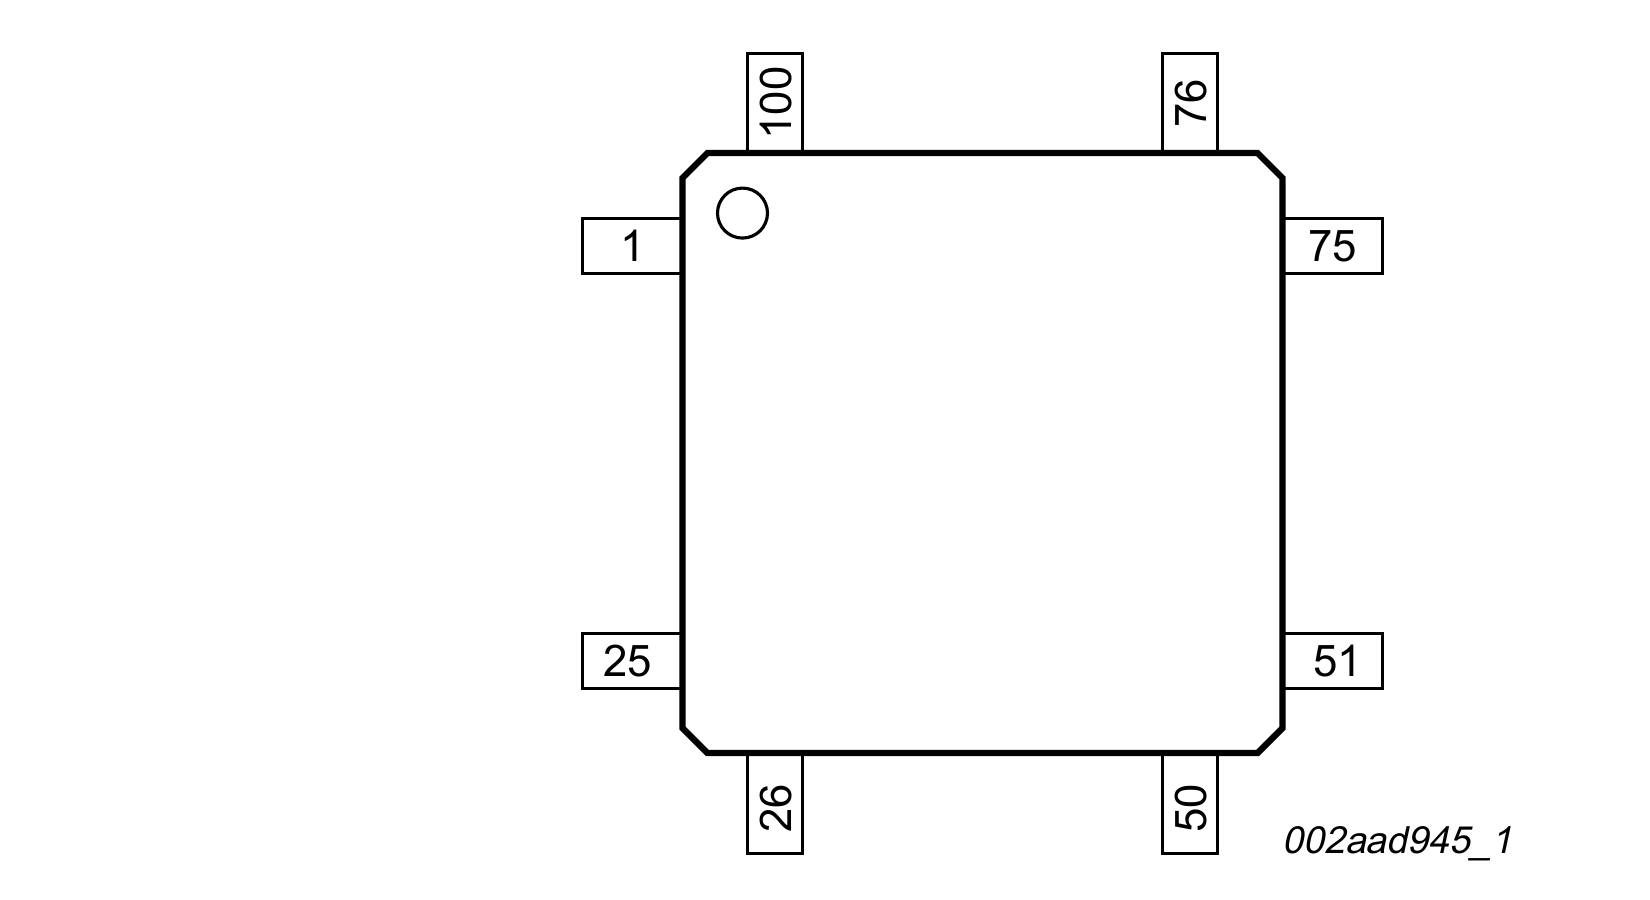
\includegraphics[width=0.94\textwidth]{images/lpc176x_lqfp100_pin_configuration_hd.png}
  \caption{Configuración de pines LQFP100 del LPC176x.}
\end{figure}

\begin{itemize}
  \item \textbf{Encapsulado de referencia:} en esta sección se usa la numeración \textbf{LQFP100}.
  \item \textbf{I/O digitales:} los pines digitales son \textit{5 V tolerant} y disponen de \textit{input hysteresis}, salvo indicación contraria en la descripción puntual.
  \item \textbf{Pines no tolerantes a 5 V:} cristal, alimentación, referencias analógicas y cualquier pin usado como entrada ADC.
  \item \textbf{Multiplexación:} cada pin puede exponer GPIO o funciones alternativas; la selección efectiva se realiza en el \textit{pin connect block}.
\end{itemize}

\subsubsection{Resumen de puertos}
\begin{table}[H]
  \centering
  \small
  \renewcommand{\arraystretch}{1.15}
  \caption{Perfil funcional de los puertos disponibles}
  \begin{tabularx}{\textwidth}{|>{\raggedright\arraybackslash}p{0.14\textwidth}|>{\raggedright\arraybackslash}X|}
    \hline
    \textbf{Puerto} & \textbf{Uso principal} \\
    \hline
    Port 0 & UART0/1/2/3, I2C1/2, SSP0/1, SPI, I2S, CAN1/2, ADC, DAC y USB. \\
    \hline
    Port 1 & Ethernet, PWM1, motor control PWM, capturas/match, USB auxiliar y ADC. \\
    \hline
    Port 2 & PWM1, UART1/2, CAN2, interrupciones externas EINT0--EINT3, NMI, trace y eventos externos. \\
    \hline
    Port 3 & Señales puntuales de timer y PWM. \\
    \hline
    Port 4 & I2S master clock, Timer 2 match y UART3. \\
    \hline
  \end{tabularx}
\end{table}

\subsubsection{Descripción de pines LPC17xx}
\noindent\textbf{Port 0.} Puerto GPIO de 32 bits con control de dirección individual. No están disponibles \texttt{P0[12]}, \texttt{P0[13]}, \texttt{P0[14]} y \texttt{P0[31]}.

\small
\renewcommand{\arraystretch}{1.15}
\setlength{\LTpre}{0pt}
\setlength{\LTpost}{8pt}

\begin{longtable}{|>{\raggedright\arraybackslash}p{0.25\textwidth}|>{\raggedright\arraybackslash}p{0.09\textwidth}|>{\raggedright\arraybackslash}p{0.08\textwidth}|>{\raggedright\arraybackslash}p{0.48\textwidth}|}
\caption{Port 0, encapsulado LQFP100}\\
\hline
\textbf{Pin / funciones} & \textbf{LQFP100} & \textbf{Tipo} & \textbf{Descripción} \\
\hline
\endfirsthead
\hline
\textbf{Pin / funciones} & \textbf{LQFP100} & \textbf{Tipo} & \textbf{Descripción} \\
\hline
\endhead
P0[0] / RD1 / TXD3 / SDA1 & 46 & I/O & GPIO general. Funciones alternativas: receptor CAN1, transmisión UART3 e I2C1 SDA. \\
\hline
P0[1] / TD1 / RXD3 / SCL1 & 47 & I/O & GPIO general. Funciones alternativas: transmisión CAN1, recepción UART3 e I2C1 SCL. \\
\hline
P0[2] / TXD0 / AD0[7] & 98 & I/O & GPIO general, transmisión UART0 o entrada ADC canal 7. En modo ADC se deshabilita la sección digital del pad. \\
\hline
P0[3] / RXD0 / AD0[6] & 99 & I/O & GPIO general, recepción UART0 o entrada ADC canal 6. En modo ADC se deshabilita la sección digital del pad. \\
\hline
P0[4] / I2SRX\_CLK / RD2 / CAP2[0] & 81 & I/O & GPIO general. Puede operar como reloj de recepción I2S, receptor CAN2 o captura Timer 2 canal 0. \\
\hline
P0[5] / I2SRX\_WS / TD2 / CAP2[1] & 80 & I/O & GPIO general. Puede operar como \textit{word select} de recepción I2S, transmisión CAN2 o captura Timer 2 canal 1. \\
\hline
P0[6] / I2SRX\_SDA / SSEL1 / MAT2[0] & 79 & I/O & GPIO general. Puede operar como dato I2S RX, selección de esclavo SSP1 o match Timer 2 canal 0. \\
\hline
P0[7] / I2STX\_CLK / SCK1 / MAT2[1] & 78 & I/O & GPIO general. Puede operar como reloj I2S TX, clock SSP1 o match Timer 2 canal 1. \\
\hline
P0[8] / I2STX\_WS / MISO1 / MAT2[2] & 77 & I/O & GPIO general. Puede operar como \textit{word select} I2S TX, MISO de SSP1 o match Timer 2 canal 2. \\
\hline
P0[9] / I2STX\_SDA / MOSI1 / MAT2[3] & 76 & I/O & GPIO general. Puede operar como dato I2S TX, MOSI de SSP1 o match Timer 2 canal 3. \\
\hline
P0[10] / TXD2 / SDA2 / MAT3[0] & 48 & I/O & GPIO general. Puede operar como transmisión UART2, I2C2 SDA o match Timer 3 canal 0. \\
\hline
P0[11] / RXD2 / SCL2 / MAT3[1] & 49 & I/O & GPIO general. Puede operar como recepción UART2, I2C2 SCL o match Timer 3 canal 1. \\
\hline
P0[15] / TXD1 / SCK0 / SCK & 62 & I/O & GPIO general. Puede operar como transmisión UART1, clock SSP0 o clock SPI. \\
\hline
P0[16] / RXD1 / SSEL0 / SSEL & 63 & I/O & GPIO general. Puede operar como recepción UART1, selección SSP0 o selección SPI. \\
\hline
P0[17] / CTS1 / MISO0 / MISO & 61 & I/O & GPIO general. Puede operar como \textit{clear-to-send} UART1, MISO de SSP0 o MISO de SPI. \\
\hline
P0[18] / DCD1 / MOSI0 / MOSI & 60 & I/O & GPIO general. Puede operar como \textit{data carrier detect} UART1, MOSI de SSP0 o MOSI de SPI. \\
\hline
P0[19] / DSR1 / SDA1 & 59 & I/O & GPIO general. Puede operar como \textit{data set ready} UART1 o I2C1 SDA. \\
\hline
P0[20] / DTR1 / SCL1 & 58 & I/O & GPIO general. Puede operar como \textit{data terminal ready} UART1 o I2C1 SCL; puede usarse como habilitación RS-485. \\
\hline
P0[21] / RI1 / RD1 & 57 & I/O & GPIO general. Puede operar como \textit{ring indicator} UART1 o receptor CAN1. \\
\hline
P0[22] / RTS1 / TD1 & 56 & I/O & GPIO general. Puede operar como \textit{request to send} UART1 o transmisión CAN1; puede usarse como habilitación RS-485. \\
\hline
P0[23] / AD0[0] / I2SRX\_CLK / CAP3[0] & 9 & I/O & GPIO general, ADC canal 0, reloj I2S RX o captura Timer 3 canal 0. En modo ADC se deshabilita la sección digital. \\
\hline
P0[24] / AD0[1] / I2SRX\_WS / CAP3[1] & 8 & I/O & GPIO general, ADC canal 1, \textit{word select} I2S RX o captura Timer 3 canal 1. En modo ADC se deshabilita la sección digital. \\
\hline
P0[25] / AD0[2] / I2SRX\_SDA / TXD3 & 7 & I/O & GPIO general, ADC canal 2, dato I2S RX o transmisión UART3. En modo ADC se deshabilita la sección digital. \\
\hline
P0[26] / AD0[3] / AOUT / RXD3 & 6 & I/O & GPIO general, ADC canal 3, salida DAC o recepción UART3. En modo ADC/DAC se deshabilita la sección digital. \\
\hline
P0[27] / SDA0 / USB\_SDA & 25 & I/O & GPIO general con pad I2C0 especializado, \textit{open-drain}, tolerante a 5 V y compatible con Standard/Fast/Fast Mode Plus. Requiere \textit{pull-up} externo. \\
\hline
P0[28] / SCL0 / USB\_SCL & 24 & I/O & GPIO general con pad I2C0 especializado, \textit{open-drain}, tolerante a 5 V y compatible con Standard/Fast/Fast Mode Plus. Requiere \textit{pull-up} externo. \\
\hline
P0[29] / USB\_D+ & 29 & I/O & GPIO general o línea bidireccional USB D+. Pad diseñado según USB 2.0 Full-speed/Low-speed. \\
\hline
P0[30] / USB\_D- & 30 & I/O & GPIO general o línea bidireccional USB D-. Pad diseñado según USB 2.0 Full-speed/Low-speed. \\
\hline
\end{longtable}

\noindent\textbf{Port 1.} Puerto GPIO de 32 bits con control de dirección individual. No están disponibles \texttt{P1[2]}, \texttt{P1[3]}, \texttt{P1[5]}, \texttt{P1[6]}, \texttt{P1[7]}, \texttt{P1[11]}, \texttt{P1[12]} y \texttt{P1[13]}.

\begin{longtable}{|>{\raggedright\arraybackslash}p{0.25\textwidth}|>{\raggedright\arraybackslash}p{0.09\textwidth}|>{\raggedright\arraybackslash}p{0.08\textwidth}|>{\raggedright\arraybackslash}p{0.48\textwidth}|}
\caption{Port 1, encapsulado LQFP100}\\
\hline
\textbf{Pin / funciones} & \textbf{LQFP100} & \textbf{Tipo} & \textbf{Descripción} \\
\hline
\endfirsthead
\hline
\textbf{Pin / funciones} & \textbf{LQFP100} & \textbf{Tipo} & \textbf{Descripción} \\
\hline
\endhead
P1[0] / ENET\_TXD0 & 95 & I/O & GPIO general o dato de transmisión Ethernet bit 0. \\
\hline
P1[1] / ENET\_TXD1 & 94 & I/O & GPIO general o dato de transmisión Ethernet bit 1. \\
\hline
P1[4] / ENET\_TX\_EN & 93 & I/O & GPIO general o habilitación de transmisión Ethernet. \\
\hline
P1[8] / ENET\_CRS & 92 & I/O & GPIO general o señal \textit{carrier sense} Ethernet. \\
\hline
P1[9] / ENET\_RXD0 & 91 & I/O & GPIO general o dato de recepción Ethernet bit 0. \\
\hline
P1[10] / ENET\_RXD1 & 90 & I/O & GPIO general o dato de recepción Ethernet bit 1. \\
\hline
P1[14] / ENET\_RX\_ER & 89 & I/O & GPIO general o error de recepción Ethernet. \\
\hline
P1[15] / ENET\_REF\_CLK & 88 & I/O & GPIO general o reloj de referencia Ethernet. \\
\hline
P1[16] / ENET\_MDC & 87 & I/O & GPIO general o clock MIIM Ethernet. \\
\hline
P1[17] / ENET\_MDIO & 86 & I/O & GPIO general o línea MIIM de datos Ethernet. \\
\hline
P1[18] / USB\_UP\_LED / PWM1[1] / CAP1[0] & 32 & I/O & GPIO general. Puede operar como LED de estado USB, salida PWM1 canal 1 o captura Timer 1 canal 0. \\
\hline
P1[19] / MCOA0 / USB\_PPWR / CAP1[1] & 33 & I/O & GPIO general. Puede operar como salida A del motor control PWM canal 0, habilitación de potencia USB o captura Timer 1 canal 1. \\
\hline
P1[20] / MCI0 / PWM1[2] / SCK0 & 34 & I/O & GPIO general. Puede operar como entrada motor control PWM/QEI PHA, PWM1 canal 2 o clock SSP0. \\
\hline
P1[21] / MCABORT / PWM1[3] / SSEL0 & 35 & I/O & GPIO general. Puede operar como aborto rápido del motor control PWM, PWM1 canal 3 o selección SSP0. \\
\hline
P1[22] / MCOB0 / USB\_PWRD / MAT1[0] & 36 & I/O & GPIO general. Puede operar como salida B del motor control PWM canal 0, estado de potencia USB o match Timer 1 canal 0. \\
\hline
P1[23] / MCI1 / PWM1[4] / MISO0 & 37 & I/O & GPIO general. Puede operar como entrada motor control PWM/QEI PHB, PWM1 canal 4 o MISO SSP0. \\
\hline
P1[24] / MCI2 / PWM1[5] / MOSI0 & 38 & I/O & GPIO general. Puede operar como entrada motor control PWM/QEI INDEX, PWM1 canal 5 o MOSI SSP0. \\
\hline
P1[25] / MCOA1 / MAT1[1] & 39 & I/O & GPIO general. Puede operar como salida A del motor control PWM canal 1 o match Timer 1 canal 1. \\
\hline
P1[26] / MCOB1 / PWM1[6] / CAP0[0] & 40 & I/O & GPIO general. Puede operar como salida B del motor control PWM canal 1, PWM1 canal 6 o captura Timer 0 canal 0. \\
\hline
P1[27] / CLKOUT / USB\_OVRCR / CAP0[1] & 43 & I/O & GPIO general. Puede operar como salida de clock, sobrecorriente USB o captura Timer 0 canal 1. \\
\hline
P1[28] / MCOA2 / PCAP1[0] / MAT0[0] & 44 & I/O & GPIO general. Puede operar como salida A del motor control PWM canal 2, captura PWM1 canal 0 o match Timer 0 canal 0. \\
\hline
P1[29] / MCOB2 / PCAP1[1] / MAT0[1] & 45 & I/O & GPIO general. Puede operar como salida B del motor control PWM canal 2, captura PWM1 canal 1 o match Timer 0 canal 1. \\
\hline
P1[30] / VBUS / AD0[4] & 21 & I/O & GPIO general o ADC canal 4. También monitorea presencia de alimentación USB; la señal debe estar en HIGH para que ocurra reset USB. \\
\hline
P1[31] / SCK1 / AD0[5] & 20 & I/O & GPIO general, clock SSP1 o ADC canal 5. En modo ADC se deshabilita la sección digital. \\
\hline
\end{longtable}

\noindent\textbf{Port 2.} Puerto GPIO de 32 bits con control de dirección individual. No están disponibles \texttt{P2[14]} a \texttt{P2[31]}.

\begin{longtable}{|>{\raggedright\arraybackslash}p{0.25\textwidth}|>{\raggedright\arraybackslash}p{0.09\textwidth}|>{\raggedright\arraybackslash}p{0.08\textwidth}|>{\raggedright\arraybackslash}p{0.48\textwidth}|}
\caption{Port 2, encapsulado LQFP100}\\
\hline
\textbf{Pin / funciones} & \textbf{LQFP100} & \textbf{Tipo} & \textbf{Descripción} \\
\hline
\endfirsthead
\hline
\textbf{Pin / funciones} & \textbf{LQFP100} & \textbf{Tipo} & \textbf{Descripción} \\
\hline
\endhead
P2[0] / PWM1[1] / TXD1 & 73 & I/O & GPIO general, PWM1 canal 1 o transmisión UART1. \\
\hline
P2[1] / PWM1[2] / RXD1 & 74 & I/O & GPIO general, PWM1 canal 2 o recepción UART1. \\
\hline
P2[2] / PWM1[3] / CTS1 / TRACEDATA[3] & 75 & I/O & GPIO general, PWM1 canal 3, \textit{clear-to-send} UART1 o dato de traza bit 3. \\
\hline
P2[3] / PWM1[4] / DCD1 / TRACEDATA[2] & 76 & I/O & GPIO general, PWM1 canal 4, \textit{data carrier detect} UART1 o dato de traza bit 2. \\
\hline
P2[4] / PWM1[5] / DSR1 / TRACEDATA[1] & 69 & I/O & GPIO general, PWM1 canal 5, \textit{data set ready} UART1 o dato de traza bit 1. \\
\hline
P2[5] / PWM1[6] / DTR1 / TRACEDATA[0] & 68 & I/O & GPIO general, PWM1 canal 6, \textit{data terminal ready} UART1 o dato de traza bit 0. \\
\hline
P2[6] / PCAP1[0] / RI1 / TRACECLK & 67 & I/O & GPIO general, captura PWM1 canal 0, \textit{ring indicator} UART1 o clock de traza. \\
\hline
P2[7] / RD2 / RTS1 & 66 & I/O & GPIO general, receptor CAN2 o \textit{request to send} UART1. \\
\hline
P2[8] / TD2 / TXD2 / ENET\_MDC & 65 & I/O & GPIO general, transmisión CAN2, transmisión UART2 o clock MIIM Ethernet. \\
\hline
P2[9] / USB\_CONNECT / RXD2 / ENET\_MDIO & 64 & I/O & GPIO general, control SoftConnect USB, recepción UART2 o línea MIIM Ethernet. \\
\hline
P2[10] / EINT0 / NMI & 53 & I/O & GPIO general con pad tolerante a 5 V y filtro de glitch de 5 ns. Puede operar como interrupción externa 0 o NMI. LOW junto con RESET fuerza modo ISP. \\
\hline
P2[11] / EINT1 / I2STX\_CLK & 52 & I/O & GPIO general con pad tolerante a 5 V y filtro de glitch de 5 ns. Puede operar como interrupción externa 1 o reloj I2S TX. \\
\hline
P2[12] / EINT2 / I2STX\_WS & 51 & I/O & GPIO general con pad tolerante a 5 V y filtro de glitch de 5 ns. Puede operar como interrupción externa 2 o \textit{word select} I2S TX. \\
\hline
P2[13] / EINT3 / I2STX\_SDA & 50 & I/O & GPIO general con pad tolerante a 5 V y filtro de glitch de 5 ns. Puede operar como interrupción externa 3 o dato I2S TX. \\
\hline
\end{longtable}

\noindent\textbf{Port 3.} Puerto GPIO de 32 bits; no están disponibles \texttt{P3[0]} a \texttt{P3[24]} ni \texttt{P3[27]} a \texttt{P3[31]}.

\begin{longtable}{|>{\raggedright\arraybackslash}p{0.25\textwidth}|>{\raggedright\arraybackslash}p{0.09\textwidth}|>{\raggedright\arraybackslash}p{0.08\textwidth}|>{\raggedright\arraybackslash}p{0.48\textwidth}|}
\caption{Port 3, encapsulado LQFP100}\\
\hline
\textbf{Pin / funciones} & \textbf{LQFP100} & \textbf{Tipo} & \textbf{Descripción} \\
\hline
\endfirsthead
\hline
\textbf{Pin / funciones} & \textbf{LQFP100} & \textbf{Tipo} & \textbf{Descripción} \\
\hline
\endhead
P3[25] / MAT0[0] / PWM1[2] & 27 & I/O & GPIO general, match Timer 0 canal 0 o PWM1 canal 2. \\
\hline
P3[26] / STCLK / MAT0[1] / PWM1[3] & 26 & I/O & GPIO general, entrada de clock SysTick, match Timer 0 canal 1 o PWM1 canal 3. \\
\hline
\end{longtable}

\noindent\textbf{Port 4.} Puerto GPIO de 32 bits; no están disponibles \texttt{P4[0]} a \texttt{P4[27]}, \texttt{P4[30]} y \texttt{P4[31]}.

\begin{longtable}{|>{\raggedright\arraybackslash}p{0.25\textwidth}|>{\raggedright\arraybackslash}p{0.09\textwidth}|>{\raggedright\arraybackslash}p{0.08\textwidth}|>{\raggedright\arraybackslash}p{0.48\textwidth}|}
\caption{Port 4, encapsulado LQFP100}\\
\hline
\textbf{Pin / funciones} & \textbf{LQFP100} & \textbf{Tipo} & \textbf{Descripción} \\
\hline
\endfirsthead
\hline
\textbf{Pin / funciones} & \textbf{LQFP100} & \textbf{Tipo} & \textbf{Descripción} \\
\hline
\endhead
P4[28] / RX\_MCLK / MAT2[0] / TXD3 & 82 & I/O & GPIO general, reloj maestro I2S RX, match Timer 2 canal 0 o transmisión UART3. \\
\hline
P4[29] / TX\_MCLK / MAT2[1] / RXD3 & 85 & I/O & GPIO general, reloj maestro I2S TX, match Timer 2 canal 1 o recepción UART3. \\
\hline
\end{longtable}

\subsubsection{Señales de depuración, reset y alimentación}
\begin{longtable}{|>{\raggedright\arraybackslash}p{0.22\textwidth}|>{\raggedright\arraybackslash}p{0.09\textwidth}|>{\raggedright\arraybackslash}p{0.08\textwidth}|>{\raggedright\arraybackslash}p{0.51\textwidth}|}
\caption{Pines especiales del encapsulado LQFP100}\\
\hline
\textbf{Señal} & \textbf{LQFP100} & \textbf{Tipo} & \textbf{Descripción} \\
\hline
\endfirsthead
\hline
\textbf{Señal} & \textbf{LQFP100} & \textbf{Tipo} & \textbf{Descripción} \\
\hline
\endhead
TDO / SWO & 1 & O & Salida JTAG TDO o salida Serial Wire Trace. \\
\hline
TDI & 2 & I & Entrada JTAG Test Data In. \\
\hline
TMS / SWDIO & 3 & I/O & Selección JTAG TMS o línea de datos Serial Wire Debug. \\
\hline
TRST & 4 & I & Reset de la interfaz JTAG. \\
\hline
TCK / SWDCLK & 5 & I & Clock JTAG o Serial Wire Debug. \\
\hline
RTCK & 100 & I/O & Señal de control de la interfaz JTAG. \\
\hline
RSTOUT & 14 & O & Salida de 3.3 V que indica estado de reset del dispositivo; refleja RESET y las fuentes internas de reset. \\
\hline
RESET & 17 & I & Entrada de reset externa. LOW reinicia el dispositivo, puertos y periféricos. Pad tolerante a 5 V con filtro de glitch de 20 ns, niveles TTL e histéresis. \\
\hline
XTAL1 & 22 & I & Entrada al oscilador principal y a los circuitos internos de generación de clock. \\
\hline
XTAL2 & 23 & O & Salida del amplificador del oscilador principal. \\
\hline
RTCX1 & 16 & I & Entrada del oscilador RTC. \\
\hline
RTCX2 & 18 & O & Salida del oscilador RTC. \\
\hline
VSS & 31, 41, 55, 72, 83, 97 & I & Referencia de tierra de 0 V. \\
\hline
VSSA & 11 & I & Tierra analógica; debe mantenerse al mismo potencial que VSS con aislamiento para reducir ruido. \\
\hline
VDD(3V3) & 28, 54, 71, 96 & I & Alimentación de 3.3 V para I/O y lógica fuera del dominio VBAT. \\
\hline
VDD(REG)(3V3) & 42, 84 & I & Alimentación de 3.3 V exclusiva del regulador interno. \\
\hline
VDDA & 10 & I & Alimentación analógica de 3.3 V para ADC y DAC; debe aislarse para minimizar ruido. \\
\hline
VREFP & 12 & I & Referencia positiva de ADC/DAC; nominalmente igual a VDDA y con aislamiento de ruido. \\
\hline
VREFN & 15 & I & Referencia negativa de ADC/DAC; nominalmente igual a VSS con aislamiento de ruido. \\
\hline
VBAT & 19 & I & Alimentación del dominio RTC. \\
\hline
n.c. & 13 & --- & Pin sin conexión interna funcional. \\
\hline
\end{longtable}

\normalsize

\IfFileExists{chapter8.tex}{\setcounter{section}{7}
\section{Pin connect block LPC17xx}
\subsection{Cómo leer este capítulo}
La \texttt{Table 74} resume qué registro \texttt{PINSELx} controla cada rango de pines del LPC17xx.

\begin{table}[H]
  \centering
  \small
  \renewcommand{\arraystretch}{1.15}
  \caption{Resumen de registros \texttt{PINSEL}}
  \begin{tabularx}{0.92\textwidth}{|>{\raggedright\arraybackslash}p{0.22\textwidth}|>{\raggedright\arraybackslash}X|>{\raggedright\arraybackslash}p{0.16\textwidth}|}
    \hline
    \textbf{Registro} & \textbf{Pines o función controlada} & \textbf{Tabla} \\
    \hline
    \texttt{PINSEL0} & \texttt{P0[15:0]} & Table 79 \\
    \hline
    \texttt{PINSEL1} & \texttt{P0[31:16]} & Table 80 \\
    \hline
    \texttt{PINSEL2} & \texttt{P1[15:0]} (Ethernet) & Table 81 \\
    \hline
    \texttt{PINSEL3} & \texttt{P1[31:16]} & Table 82 \\
    \hline
    \texttt{PINSEL4} & \texttt{P2[15:0]} & Table 83 \\
    \hline
    \texttt{PINSEL5} & \texttt{P2[31:16]} & No usado \\
    \hline
    \texttt{PINSEL6} & \texttt{P3[15:0]} & No usado \\
    \hline
    \texttt{PINSEL7} & \texttt{P3[31:16]} & Table 84 \\
    \hline
    \texttt{PINSEL8} & \texttt{P4[15:0]} & No usado \\
    \hline
    \texttt{PINSEL9} & \texttt{P4[31:16]} & Table 85 \\
    \hline
    \texttt{PINSEL10} & Habilitación del puerto de traza & Table 86 \\
    \hline
  \end{tabularx}
\end{table}

\subsection{Descripción}
El \textit{pin connect block} permite que la mayoría de los pines del microcontrolador expongan más de una función potencial. Los registros de configuración gobiernan los multiplexores que conectan el pin físico con los periféricos internos.

Los periféricos deben conectarse a los pines apropiados antes de habilitarlos y antes de habilitar sus interrupciones asociadas. La actividad de una función periférica activa que no esté mapeada a un pin relacionado debe considerarse indefinida.

Seleccionar una única función en un pin excluye las demás funciones periféricas disponibles sobre ese mismo pin. Aun así, la entrada GPIO permanece conectada y puede leerse por software o contribuir al sistema de interrupciones GPIO.

\subsection{Valores de selección de función de pin}
Los registros \texttt{PINSEL} controlan la función expuesta por cada pin. Cada par de bits de \texttt{PINSEL0} a \texttt{PINSEL9} corresponde a un pin específico.

\begin{table}[H]
  \centering
  \small
  \renewcommand{\arraystretch}{1.15}
  \caption{Bits de selección de función de pin}
  \begin{tabularx}{0.9\textwidth}{|>{\raggedright\arraybackslash}p{0.16\textwidth}|>{\raggedright\arraybackslash}X|>{\raggedright\arraybackslash}p{0.18\textwidth}|}
    \hline
    \textbf{Valor en \texttt{PINSEL0} a \texttt{PINSEL9}} & \textbf{Función} & \textbf{Valor tras reset} \\
    \hline
    \texttt{00} & Función primaria, normalmente GPIO. & \texttt{00} \\
    \hline
    \texttt{01} & Primera función alternativa. & --- \\
    \hline
    \texttt{10} & Segunda función alternativa. & --- \\
    \hline
    \texttt{11} & Tercera función alternativa. & --- \\
    \hline
  \end{tabularx}
\end{table}

El bit de dirección en los registros GPIO sólo tiene efecto cuando el pin está configurado como GPIO. Para las demás funciones la dirección queda controlada automáticamente por el periférico.

\paragraph{Conexiones múltiples}
Una misma función periférica puede estar disponible en más de un pin. Si una salida periférica se asigna a varios pines, la señal aparece en todos ellos. Si una entrada periférica se asigna a varios pines, el periférico toma la señal del pin con menor número de puerto y, dentro del mismo puerto, del pin con menor número.

\subsection{Valores de selección del modo de pin}
Los registros \texttt{PINMODE} controlan el modo de entrada de todos los puertos. Esto incluye las resistencias internas \textit{pull-up}/\textit{pull-down} y el modo especial \textit{open-drain}. La selección de \textit{pull-up}/\textit{pull-down} aplica a cualquier función del pin salvo en los pines \texttt{I2C0} y USB. El modo efectivo usa tres bits por pin: dos bits en \texttt{PINMODE} y un bit adicional en \texttt{PINMODE\_OD}.

\begin{table}[H]
  \centering
  \small
  \renewcommand{\arraystretch}{1.15}
  \caption{Bits de selección de modo de pin}
  \begin{tabularx}{0.9\textwidth}{|>{\raggedright\arraybackslash}p{0.16\textwidth}|>{\raggedright\arraybackslash}X|>{\raggedright\arraybackslash}p{0.18\textwidth}|}
    \hline
    \textbf{Valor en \texttt{PINMODE0} a \texttt{PINMODE9}} & \textbf{Función} & \textbf{Valor tras reset} \\
    \hline
    \texttt{00} & Resistencia interna \textit{pull-up} habilitada. & \texttt{00} \\
    \hline
    \texttt{01} & Modo \textit{repeater}. & --- \\
    \hline
    \texttt{10} & Sin \textit{pull-up} ni \textit{pull-down}. & --- \\
    \hline
    \texttt{11} & Resistencia interna \textit{pull-down} habilitada. & --- \\
    \hline
  \end{tabularx}
\end{table}

\begin{itemize}
  \item \textbf{\textit{Pull-up}:} polariza el pin a nivel alto cuando no hay conducción externa.
  \item \textbf{\textit{Pull-down}:} polariza el pin a nivel bajo cuando no hay conducción externa.
  \item \textbf{\textit{Neither}:} deja el nodo sin polarización interna; sólo conviene cuando existe una red externa definida.
  \item \textbf{\textit{Repeater}:} habilita \textit{pull-up} si el pin está en alto y \textit{pull-down} si está en bajo, reteniendo el último estado conocido mientras el pin sea entrada y no esté manejado externamente.
  \item \textbf{Límite de \textit{repeater}:} la retención no aplica en \textit{Deep Power-down}.
\end{itemize}

Los registros \texttt{PINMODE\_OD} controlan el modo \textit{open-drain}. Cuando un pin configurado como salida escribe \texttt{0}, el pad conduce a masa. Cuando escribe \texttt{1}, el driver de salida se desactiva, equivalente a liberar el pin. Así se emula una salida de drenador abierto.

\begin{table}[H]
  \centering
  \small
  \renewcommand{\arraystretch}{1.15}
  \caption{Bits de selección de modo \textit{open-drain}}
  \begin{tabularx}{0.9\textwidth}{|>{\raggedright\arraybackslash}p{0.22\textwidth}|>{\raggedright\arraybackslash}X|>{\raggedright\arraybackslash}p{0.18\textwidth}|}
    \hline
    \textbf{Valor en \texttt{PINMODE\_OD0} a \texttt{PINMODE\_OD4}} & \textbf{Función} & \textbf{Valor tras reset} \\
    \hline
    \texttt{0} & Modo normal, no \textit{open-drain}. & \texttt{0} \\
    \hline
    \texttt{1} & Modo \textit{open-drain}. & --- \\
    \hline
  \end{tabularx}
\end{table}

\paragraph{Efecto de \texttt{PINMODE} en \textit{open-drain}}
El valor de \texttt{PINMODE} normalmente sólo aplica cuando el pin es entrada. En \textit{open-drain}, ese modo no aplica mientras el pin está conduciendo un \texttt{0}. En cambio, cuando el pin vale \texttt{1} y el driver queda apagado, la configuración de \texttt{PINMODE} vuelve a ser efectiva. Esto permite, por ejemplo, una salida \textit{open-drain} con \textit{pull-up} interno activo sólo cuando el pin no está forzando el nivel bajo.

\subsection{Descripción de registros}
El módulo de control de pines incluye los registros de selección de función, modo de entrada, modo \textit{open-drain} y configuración especial del bloque \texttt{I2C0}.

\begin{longtable}{|>{\raggedright\arraybackslash}p{0.18\textwidth}|>{\raggedright\arraybackslash}p{0.34\textwidth}|>{\centering\arraybackslash}p{0.08\textwidth}|>{\centering\arraybackslash}p{0.12\textwidth}|>{\raggedright\arraybackslash}p{0.18\textwidth}|}
\caption{Mapa de registros del Pin Connect Block}\\
\hline
\textbf{Nombre} & \textbf{Descripción} & \textbf{Acceso} & \textbf{Reset} & \textbf{Dirección} \\
\hline
\endfirsthead
\hline
\textbf{Nombre} & \textbf{Descripción} & \textbf{Acceso} & \textbf{Reset} & \textbf{Dirección} \\
\hline
\endhead
\texttt{PINSEL0} & Pin function select register 0. & R/W & \texttt{0} & \texttt{0x4002 C000} \\
\hline
\texttt{PINSEL1} & Pin function select register 1. & R/W & \texttt{0} & \texttt{0x4002 C004} \\
\hline
\texttt{PINSEL2} & Pin function select register 2. & R/W & \texttt{0} & \texttt{0x4002 C008} \\
\hline
\texttt{PINSEL3} & Pin function select register 3. & R/W & \texttt{0} & \texttt{0x4002 C00C} \\
\hline
\texttt{PINSEL4} & Pin function select register 4. & R/W & \texttt{0} & \texttt{0x4002 C010} \\
\hline
\texttt{PINSEL7} & Pin function select register 7. & R/W & \texttt{0} & \texttt{0x4002 C01C} \\
\hline
\texttt{PINSEL8} & Pin function select register 8. & R/W & \texttt{0} & \texttt{0x4002 C020} \\
\hline
\texttt{PINSEL9} & Pin function select register 9. & R/W & \texttt{0} & \texttt{0x4002 C024} \\
\hline
\texttt{PINSEL10} & Pin function select register 10. & R/W & \texttt{0} & \texttt{0x4002 C028} \\
\hline
\texttt{PINMODE0} & Pin mode select register 0. & R/W & \texttt{0} & \texttt{0x4002 C040} \\
\hline
\texttt{PINMODE1} & Pin mode select register 1. & R/W & \texttt{0} & \texttt{0x4002 C044} \\
\hline
\texttt{PINMODE2} & Pin mode select register 2. & R/W & \texttt{0} & \texttt{0x4002 C048} \\
\hline
\texttt{PINMODE3} & Pin mode select register 3. & R/W & \texttt{0} & \texttt{0x4002 C04C} \\
\hline
\texttt{PINMODE4} & Pin mode select register 4. & R/W & \texttt{0} & \texttt{0x4002 C050} \\
\hline
\texttt{PINMODE5} & Pin mode select register 5. & R/W & \texttt{0} & \texttt{0x4002 C054} \\
\hline
\texttt{PINMODE6} & Pin mode select register 6. & R/W & \texttt{0} & \texttt{0x4002 C058} \\
\hline
\texttt{PINMODE7} & Pin mode select register 7. & R/W & \texttt{0} & \texttt{0x4002 C05C} \\
\hline
\texttt{PINMODE9} & Pin mode select register 9. & R/W & \texttt{0} & \texttt{0x4002 C064} \\
\hline
\texttt{PINMODE\_OD0} & Open drain mode control register 0. & R/W & \texttt{0} & \texttt{0x4002 C068} \\
\hline
\texttt{PINMODE\_OD1} & Open drain mode control register 1. & R/W & \texttt{0} & \texttt{0x4002 C06C} \\
\hline
\texttt{PINMODE\_OD2} & Open drain mode control register 2. & R/W & \texttt{0} & \texttt{0x4002 C070} \\
\hline
\texttt{PINMODE\_OD3} & Open drain mode control register 3. & R/W & \texttt{0} & \texttt{0x4002 C074} \\
\hline
\texttt{PINMODE\_OD4} & Open drain mode control register 4. & R/W & \texttt{0} & \texttt{0x4002 C078} \\
\hline
\texttt{I2CPADCFG} & I2C Pin Configuration register. & R/W & \texttt{0} & \texttt{0x4002 C07C} \\
\hline
\end{longtable}

\noindent\textit{Nota:} el valor de reset refleja sólo los bits usados; no incluye el contenido de bits reservados. Ante \textit{external reset}, \textit{watchdog reset}, \textit{power-on reset} y \textit{BOD reset}, todos los registros del módulo vuelven a \texttt{0}.

\scriptsize
\renewcommand{\arraystretch}{1.12}
\setlength{\LTpre}{4pt}
\setlength{\LTpost}{10pt}

\subsubsection{Pin Function Select register 0 (\texttt{PINSEL0} - \texttt{0x4002 C000})}
Controla la mitad baja del puerto 0. El bit de dirección en \texttt{FIO0DIR} sólo es efectivo cuando se selecciona la función GPIO.

\begin{longtable}{|>{\raggedright\arraybackslash}p{0.08\textwidth}|>{\raggedright\arraybackslash}p{0.09\textwidth}|>{\raggedright\arraybackslash}p{0.16\textwidth}|>{\raggedright\arraybackslash}p{0.14\textwidth}|>{\raggedright\arraybackslash}p{0.14\textwidth}|>{\raggedright\arraybackslash}p{0.14\textwidth}|>{\centering\arraybackslash}p{0.07\textwidth}|}
\caption{Pin function select register 0 (\texttt{PINSEL0}) bit description}\\
\hline
\textbf{Bits} & \textbf{Pin} & \textbf{Función 00} & \textbf{Función 01} & \textbf{Función 10} & \textbf{Función 11} & \textbf{Reset} \\
\hline
\endfirsthead
\hline
\textbf{Bits} & \textbf{Pin} & \textbf{Función 00} & \textbf{Función 01} & \textbf{Función 10} & \textbf{Función 11} & \textbf{Reset} \\
\hline
\endhead
\texttt{1:0} & \texttt{P0.0} & GPIO Port 0.0 & \texttt{RD1} & \texttt{TXD3} & \texttt{SDA1} & \texttt{00} \\
\hline
\texttt{3:2} & \texttt{P0.1} & GPIO Port 0.1 & \texttt{TD1} & \texttt{RXD3} & \texttt{SCL1} & \texttt{00} \\
\hline
\texttt{5:4} & \texttt{P0.2} & GPIO Port 0.2 & \texttt{TXD0} & \texttt{AD0.7} & Reserved & \texttt{00} \\
\hline
\texttt{7:6} & \texttt{P0.3} & GPIO Port 0.3 & \texttt{RXD0} & \texttt{AD0.6} & Reserved & \texttt{00} \\
\hline
\texttt{9:8} & \texttt{P0.4[1]} & GPIO Port 0.4 & \texttt{I2SRX\_CLK} & \texttt{RD2} & \texttt{CAP2.0} & \texttt{00} \\
\hline
\texttt{11:10} & \texttt{P0.5[1]} & GPIO Port 0.5 & \texttt{I2SRX\_WS} & \texttt{TD2} & \texttt{CAP2.1} & \texttt{00} \\
\hline
\texttt{13:12} & \texttt{P0.6} & GPIO Port 0.6 & \texttt{I2SRX\_SDA} & \texttt{SSEL1} & \texttt{MAT2.0} & \texttt{00} \\
\hline
\texttt{15:14} & \texttt{P0.7} & GPIO Port 0.7 & \texttt{I2STX\_CLK} & \texttt{SCK1} & \texttt{MAT2.1} & \texttt{00} \\
\hline
\texttt{17:16} & \texttt{P0.8} & GPIO Port 0.8 & \texttt{I2STX\_WS} & \texttt{MISO1} & \texttt{MAT2.2} & \texttt{00} \\
\hline
\texttt{19:18} & \texttt{P0.9} & GPIO Port 0.9 & \texttt{I2STX\_SDA} & \texttt{MOSI1} & \texttt{MAT2.3} & \texttt{00} \\
\hline
\texttt{21:20} & \texttt{P0.10} & GPIO Port 0.10 & \texttt{TXD2} & \texttt{SDA2} & \texttt{MAT3.0} & \texttt{00} \\
\hline
\texttt{23:22} & \texttt{P0.11} & GPIO Port 0.11 & \texttt{RXD2} & \texttt{SCL2} & \texttt{MAT3.1} & \texttt{00} \\
\hline
\texttt{29:24} & --- & Reserved & Reserved & Reserved & Reserved & \texttt{0} \\
\hline
\texttt{31:30} & \texttt{P0.15} & GPIO Port 0.15 & \texttt{TXD1} & \texttt{SCK0} & \texttt{SCK} & \texttt{00} \\
\hline
\end{longtable}
\noindent\textit{[1] No disponible en encapsulado de 80 pines.}

\subsubsection{Pin Function Select register 1 (\texttt{PINSEL1} - \texttt{0x4002 C004})}
Controla la mitad alta del puerto 0.

\begin{longtable}{|>{\raggedright\arraybackslash}p{0.08\textwidth}|>{\raggedright\arraybackslash}p{0.09\textwidth}|>{\raggedright\arraybackslash}p{0.16\textwidth}|>{\raggedright\arraybackslash}p{0.14\textwidth}|>{\raggedright\arraybackslash}p{0.14\textwidth}|>{\raggedright\arraybackslash}p{0.14\textwidth}|>{\centering\arraybackslash}p{0.07\textwidth}|}
\caption{Pin function select register 1 (\texttt{PINSEL1}) bit description}\\
\hline
\textbf{Bits} & \textbf{Pin} & \textbf{Función 00} & \textbf{Función 01} & \textbf{Función 10} & \textbf{Función 11} & \textbf{Reset} \\
\hline
\endfirsthead
\hline
\textbf{Bits} & \textbf{Pin} & \textbf{Función 00} & \textbf{Función 01} & \textbf{Función 10} & \textbf{Función 11} & \textbf{Reset} \\
\hline
\endhead
\texttt{1:0} & \texttt{P0.16} & GPIO Port 0.16 & \texttt{RXD1} & \texttt{SSEL0} & \texttt{SSEL} & \texttt{00} \\
\hline
\texttt{3:2} & \texttt{P0.17} & GPIO Port 0.17 & \texttt{CTS1} & \texttt{MISO0} & \texttt{MISO} & \texttt{00} \\
\hline
\texttt{5:4} & \texttt{P0.18} & GPIO Port 0.18 & \texttt{DCD1} & \texttt{MOSI0} & \texttt{MOSI} & \texttt{00} \\
\hline
\texttt{7:6} & \texttt{P0.19[1]} & GPIO Port 0.19 & \texttt{DSR1} & Reserved & \texttt{SDA1} & \texttt{00} \\
\hline
\texttt{9:8} & \texttt{P0.20[1]} & GPIO Port 0.20 & \texttt{DTR1} & Reserved & \texttt{SCL1} & \texttt{00} \\
\hline
\texttt{11:10} & \texttt{P0.21[1]} & GPIO Port 0.21 & \texttt{RI1} & Reserved & \texttt{RD1} & \texttt{00} \\
\hline
\texttt{13:12} & \texttt{P0.22} & GPIO Port 0.22 & \texttt{RTS1} & Reserved & \texttt{TD1} & \texttt{00} \\
\hline
\texttt{15:14} & \texttt{P0.23[1]} & GPIO Port 0.23 & \texttt{AD0.0} & \texttt{I2SRX\_CLK} & \texttt{CAP3.0} & \texttt{00} \\
\hline
\texttt{17:16} & \texttt{P0.24[1]} & GPIO Port 0.24 & \texttt{AD0.1} & \texttt{I2SRX\_WS} & \texttt{CAP3.1} & \texttt{00} \\
\hline
\texttt{19:18} & \texttt{P0.25} & GPIO Port 0.25 & \texttt{AD0.2} & \texttt{I2SRX\_SDA} & \texttt{TXD3} & \texttt{00} \\
\hline
\texttt{21:20} & \texttt{P0.26} & GPIO Port 0.26 & \texttt{AD0.3} & \texttt{AOUT} & \texttt{RXD3} & \texttt{00} \\
\hline
\texttt{23:22} & \texttt{P0.27[1][2]} & GPIO Port 0.27 & \texttt{SDA0} & \texttt{USB\_SDA} & Reserved & \texttt{00} \\
\hline
\texttt{25:24} & \texttt{P0.28[1][2]} & GPIO Port 0.28 & \texttt{SCL0} & \texttt{USB\_SCL} & Reserved & \texttt{00} \\
\hline
\texttt{27:26} & \texttt{P0.29} & GPIO Port 0.29 & \texttt{USB\_D+} & Reserved & Reserved & \texttt{00} \\
\hline
\texttt{29:28} & \texttt{P0.30} & GPIO Port 0.30 & \texttt{USB\_D-} & Reserved & Reserved & \texttt{00} \\
\hline
\texttt{31:30} & --- & Reserved & Reserved & Reserved & Reserved & \texttt{00} \\
\hline
\end{longtable}
\noindent\textit{[1] No disponible en encapsulado de 80 pines.}\\
\textit{[2] \texttt{P0.27} y \texttt{P0.28} son pines \textit{open-drain} para compatibilidad con bus I\textsuperscript{2}C.}

\subsubsection{Pin Function Select register 2 (\texttt{PINSEL2} - \texttt{0x4002 C008})}
Controla la mitad baja del puerto 1, asociada principalmente a señales Ethernet.

\begin{longtable}{|>{\raggedright\arraybackslash}p{0.08\textwidth}|>{\raggedright\arraybackslash}p{0.09\textwidth}|>{\raggedright\arraybackslash}p{0.16\textwidth}|>{\raggedright\arraybackslash}p{0.14\textwidth}|>{\raggedright\arraybackslash}p{0.14\textwidth}|>{\raggedright\arraybackslash}p{0.14\textwidth}|>{\centering\arraybackslash}p{0.07\textwidth}|}
\caption{Pin function select register 2 (\texttt{PINSEL2}) bit description}\\
\hline
\textbf{Bits} & \textbf{Pin} & \textbf{Función 00} & \textbf{Función 01} & \textbf{Función 10} & \textbf{Función 11} & \textbf{Reset} \\
\hline
\endfirsthead
\hline
\textbf{Bits} & \textbf{Pin} & \textbf{Función 00} & \textbf{Función 01} & \textbf{Función 10} & \textbf{Función 11} & \textbf{Reset} \\
\hline
\endhead
\texttt{1:0} & \texttt{P1.0} & GPIO Port 1.0 & \texttt{ENET\_TXD0} & Reserved & Reserved & \texttt{00} \\
\hline
\texttt{3:2} & \texttt{P1.1} & GPIO Port 1.1 & \texttt{ENET\_TXD1} & Reserved & Reserved & \texttt{00} \\
\hline
\texttt{7:4} & --- & Reserved & Reserved & Reserved & Reserved & \texttt{0} \\
\hline
\texttt{9:8} & \texttt{P1.4} & GPIO Port 1.4 & \texttt{ENET\_TX\_EN} & Reserved & Reserved & \texttt{00} \\
\hline
\texttt{15:10} & --- & Reserved & Reserved & Reserved & Reserved & \texttt{0} \\
\hline
\texttt{17:16} & \texttt{P1.8} & GPIO Port 1.8 & \texttt{ENET\_CRS} & Reserved & Reserved & \texttt{00} \\
\hline
\texttt{19:18} & \texttt{P1.9} & GPIO Port 1.9 & \texttt{ENET\_RXD0} & Reserved & Reserved & \texttt{00} \\
\hline
\texttt{21:20} & \texttt{P1.10} & GPIO Port 1.10 & \texttt{ENET\_RXD1} & Reserved & Reserved & \texttt{00} \\
\hline
\texttt{27:22} & --- & Reserved & Reserved & Reserved & Reserved & \texttt{0} \\
\hline
\texttt{29:28} & \texttt{P1.14} & GPIO Port 1.14 & \texttt{ENET\_RX\_ER} & Reserved & Reserved & \texttt{00} \\
\hline
\texttt{31:30} & \texttt{P1.15} & GPIO Port 1.15 & \texttt{ENET\_REF\_CLK} & Reserved & Reserved & \texttt{00} \\
\hline
\end{longtable}

\subsubsection{Pin Function Select register 3 (\texttt{PINSEL3} - \texttt{0x4002 C00C})}
Controla la mitad alta del puerto 1.

\begin{longtable}{|>{\raggedright\arraybackslash}p{0.08\textwidth}|>{\raggedright\arraybackslash}p{0.09\textwidth}|>{\raggedright\arraybackslash}p{0.16\textwidth}|>{\raggedright\arraybackslash}p{0.14\textwidth}|>{\raggedright\arraybackslash}p{0.14\textwidth}|>{\raggedright\arraybackslash}p{0.14\textwidth}|>{\centering\arraybackslash}p{0.07\textwidth}|}
\caption{Pin function select register 3 (\texttt{PINSEL3}) bit description}\\
\hline
\textbf{Bits} & \textbf{Pin} & \textbf{Función 00} & \textbf{Función 01} & \textbf{Función 10} & \textbf{Función 11} & \textbf{Reset} \\
\hline
\endfirsthead
\hline
\textbf{Bits} & \textbf{Pin} & \textbf{Función 00} & \textbf{Función 01} & \textbf{Función 10} & \textbf{Función 11} & \textbf{Reset} \\
\hline
\endhead
\texttt{1:0} & \texttt{P1.16[1]} & GPIO Port 1.16 & \texttt{ENET\_MDC} & Reserved & Reserved & \texttt{00} \\
\hline
\texttt{3:2} & \texttt{P1.17[1]} & GPIO Port 1.17 & \texttt{ENET\_MDIO} & Reserved & Reserved & \texttt{00} \\
\hline
\texttt{5:4} & \texttt{P1.18} & GPIO Port 1.18 & \texttt{USB\_UP\_LED} & \texttt{PWM1.1} & \texttt{CAP1.0} & \texttt{00} \\
\hline
\texttt{7:6} & \texttt{P1.19} & GPIO Port 1.19 & \texttt{MCOA0} & \texttt{USB\_PPWR} & \texttt{CAP1.1} & \texttt{00} \\
\hline
\texttt{9:8} & \texttt{P1.20} & GPIO Port 1.20 & \texttt{MCI0} & \texttt{PWM1.2} & \texttt{SCK0} & \texttt{00} \\
\hline
\texttt{11:10} & \texttt{P1.21[1]} & GPIO Port 1.21 & \texttt{MCABORT} & \texttt{PWM1.3} & \texttt{SSEL0} & \texttt{00} \\
\hline
\texttt{13:12} & \texttt{P1.22} & GPIO Port 1.22 & \texttt{MCOB0} & \texttt{USB\_PWRD} & \texttt{MAT1.0} & \texttt{00} \\
\hline
\texttt{15:14} & \texttt{P1.23} & GPIO Port 1.23 & \texttt{MCI1} & \texttt{PWM1.4} & \texttt{MISO0} & \texttt{00} \\
\hline
\texttt{17:16} & \texttt{P1.24} & GPIO Port 1.24 & \texttt{MCI2} & \texttt{PWM1.5} & \texttt{MOSI0} & \texttt{00} \\
\hline
\texttt{19:18} & \texttt{P1.25} & GPIO Port 1.25 & \texttt{MCOA1} & Reserved & \texttt{MAT1.1} & \texttt{00} \\
\hline
\texttt{21:20} & \texttt{P1.26} & GPIO Port 1.26 & \texttt{MCOB1} & \texttt{PWM1.6} & \texttt{CAP0.0} & \texttt{00} \\
\hline
\texttt{23:22} & \texttt{P1.27[1]} & GPIO Port 1.27 & \texttt{CLKOUT} & \texttt{USB\_OVRCR} & \texttt{CAP0.1} & \texttt{00} \\
\hline
\texttt{25:24} & \texttt{P1.28} & GPIO Port 1.28 & \texttt{MCOA2} & \texttt{PCAP1.0} & \texttt{MAT0.0} & \texttt{00} \\
\hline
\texttt{27:26} & \texttt{P1.29} & GPIO Port 1.29 & \texttt{MCOB2} & \texttt{PCAP1.1} & \texttt{MAT0.1} & \texttt{00} \\
\hline
\texttt{29:28} & \texttt{P1.30} & GPIO Port 1.30 & Reserved & \texttt{VBUS} & \texttt{AD0.4} & \texttt{00} \\
\hline
\texttt{31:30} & \texttt{P1.31} & GPIO Port 1.31 & Reserved & \texttt{SCK1} & \texttt{AD0.5} & \texttt{00} \\
\hline
\end{longtable}
\noindent\textit{[1] No disponible en encapsulado de 80 pines.}

\subsubsection{Pin Function Select register 4 (\texttt{PINSEL4} - \texttt{0x4002 C010})}
Controla la mitad baja del puerto 2.

\begin{longtable}{|>{\raggedright\arraybackslash}p{0.08\textwidth}|>{\raggedright\arraybackslash}p{0.09\textwidth}|>{\raggedright\arraybackslash}p{0.16\textwidth}|>{\raggedright\arraybackslash}p{0.14\textwidth}|>{\raggedright\arraybackslash}p{0.14\textwidth}|>{\raggedright\arraybackslash}p{0.14\textwidth}|>{\centering\arraybackslash}p{0.07\textwidth}|}
\caption{Pin function select register 4 (\texttt{PINSEL4}) bit description}\\
\hline
\textbf{Bits} & \textbf{Pin} & \textbf{Función 00} & \textbf{Función 01} & \textbf{Función 10} & \textbf{Función 11} & \textbf{Reset} \\
\hline
\endfirsthead
\hline
\textbf{Bits} & \textbf{Pin} & \textbf{Función 00} & \textbf{Función 01} & \textbf{Función 10} & \textbf{Función 11} & \textbf{Reset} \\
\hline
\endhead
\texttt{1:0} & \texttt{P2.0} & GPIO Port 2.0 & \texttt{PWM1.1} & \texttt{TXD1} & Reserved & \texttt{00} \\
\hline
\texttt{3:2} & \texttt{P2.1} & GPIO Port 2.1 & \texttt{PWM1.2} & \texttt{RXD1} & Reserved & \texttt{00} \\
\hline
\texttt{5:4} & \texttt{P2.2} & GPIO Port 2.2 & \texttt{PWM1.3} & \texttt{CTS1} & Reserved [2] & \texttt{00} \\
\hline
\texttt{7:6} & \texttt{P2.3} & GPIO Port 2.3 & \texttt{PWM1.4} & \texttt{DCD1} & Reserved [2] & \texttt{00} \\
\hline
\texttt{9:8} & \texttt{P2.4} & GPIO Port 2.4 & \texttt{PWM1.5} & \texttt{DSR1} & Reserved [2] & \texttt{00} \\
\hline
\texttt{11:10} & \texttt{P2.5} & GPIO Port 2.5 & \texttt{PWM1.6} & \texttt{DTR1} & Reserved [2] & \texttt{00} \\
\hline
\texttt{13:12} & \texttt{P2.6} & GPIO Port 2.6 & \texttt{PCAP1.0} & \texttt{RI1} & Reserved [2] & \texttt{00} \\
\hline
\texttt{15:14} & \texttt{P2.7} & GPIO Port 2.7 & \texttt{RD2} & \texttt{RTS1} & Reserved & \texttt{00} \\
\hline
\texttt{17:16} & \texttt{P2.8} & GPIO Port 2.8 & \texttt{TD2} & \texttt{TXD2} & \texttt{ENET\_MDC} & \texttt{00} \\
\hline
\texttt{19:18} & \texttt{P2.9} & GPIO Port 2.9 & \texttt{USB\_CONNECT} & \texttt{RXD2} & \texttt{ENET\_MDIO} & \texttt{00} \\
\hline
\texttt{21:20} & \texttt{P2.10} & GPIO Port 2.10 & \texttt{EINT0} & \texttt{NMI} & Reserved & \texttt{00} \\
\hline
\texttt{23:22} & \texttt{P2.11[1]} & GPIO Port 2.11 & \texttt{EINT1} & Reserved & \texttt{I2STX\_CLK} & \texttt{00} \\
\hline
\texttt{25:24} & \texttt{P2.12[1]} & GPIO Port 2.12 & \texttt{EINT2} & Reserved & \texttt{I2STX\_WS} & \texttt{00} \\
\hline
\texttt{27:26} & \texttt{P2.13[1]} & GPIO Port 2.13 & \texttt{EINT3} & Reserved & \texttt{I2STX\_SDA} & \texttt{00} \\
\hline
\texttt{31:28} & --- & Reserved & Reserved & Reserved & Reserved & \texttt{0} \\
\hline
\end{longtable}
\noindent\textit{[1] No disponible en encapsulado de 80 pines.}\\
\textit{[2] Estos pines también soportan traza de depuración al seleccionarse vía herramienta de desarrollo o escribiendo en \texttt{PINSEL10}.}

\subsubsection{Pin Function Select register 7 (\texttt{PINSEL7} - \texttt{0x4002 C01C})}
Controla la mitad alta del puerto 3.

\begin{longtable}{|>{\raggedright\arraybackslash}p{0.08\textwidth}|>{\raggedright\arraybackslash}p{0.09\textwidth}|>{\raggedright\arraybackslash}p{0.16\textwidth}|>{\raggedright\arraybackslash}p{0.14\textwidth}|>{\raggedright\arraybackslash}p{0.14\textwidth}|>{\raggedright\arraybackslash}p{0.14\textwidth}|>{\centering\arraybackslash}p{0.07\textwidth}|}
\caption{Pin function select register 7 (\texttt{PINSEL7}) bit description}\\
\hline
\textbf{Bits} & \textbf{Pin} & \textbf{Función 00} & \textbf{Función 01} & \textbf{Función 10} & \textbf{Función 11} & \textbf{Reset} \\
\hline
\endfirsthead
\hline
\textbf{Bits} & \textbf{Pin} & \textbf{Función 00} & \textbf{Función 01} & \textbf{Función 10} & \textbf{Función 11} & \textbf{Reset} \\
\hline
\endhead
\texttt{17:0} & --- & Reserved & Reserved & Reserved & Reserved & \texttt{0} \\
\hline
\texttt{19:18} & \texttt{P3.25[1]} & GPIO Port 3.25 & Reserved & \texttt{MAT0.0} & \texttt{PWM1.2} & \texttt{00} \\
\hline
\texttt{21:20} & \texttt{P3.26[1]} & GPIO Port 3.26 & \texttt{STCLK} & \texttt{MAT0.1} & \texttt{PWM1.3} & \texttt{00} \\
\hline
\texttt{31:22} & --- & Reserved & Reserved & Reserved & Reserved & \texttt{0} \\
\hline
\end{longtable}
\noindent\textit{[1] No disponible en encapsulado de 80 pines.}

\subsubsection{Pin Function Select register 9 (\texttt{PINSEL9} - \texttt{0x4002 C024})}
Controla la mitad alta del puerto 4.

\begin{longtable}{|>{\raggedright\arraybackslash}p{0.08\textwidth}|>{\raggedright\arraybackslash}p{0.09\textwidth}|>{\raggedright\arraybackslash}p{0.16\textwidth}|>{\raggedright\arraybackslash}p{0.14\textwidth}|>{\raggedright\arraybackslash}p{0.14\textwidth}|>{\raggedright\arraybackslash}p{0.14\textwidth}|>{\centering\arraybackslash}p{0.07\textwidth}|}
\caption{Pin function select register 9 (\texttt{PINSEL9}) bit description}\\
\hline
\textbf{Bits} & \textbf{Pin} & \textbf{Función 00} & \textbf{Función 01} & \textbf{Función 10} & \textbf{Función 11} & \textbf{Reset} \\
\hline
\endfirsthead
\hline
\textbf{Bits} & \textbf{Pin} & \textbf{Función 00} & \textbf{Función 01} & \textbf{Función 10} & \textbf{Función 11} & \textbf{Reset} \\
\hline
\endhead
\texttt{23:0} & --- & Reserved & Reserved & Reserved & Reserved & \texttt{00} \\
\hline
\texttt{25:24} & \texttt{P4.28} & GPIO Port 4.28 & \texttt{RX\_MCLK} & \texttt{MAT2.0} & \texttt{TXD3} & \texttt{00} \\
\hline
\texttt{27:26} & \texttt{P4.29} & GPIO Port 4.29 & \texttt{TX\_MCLK} & \texttt{MAT2.1} & \texttt{RXD3} & \texttt{00} \\
\hline
\texttt{31:28} & --- & Reserved & Reserved & Reserved & Reserved & \texttt{00} \\
\hline
\end{longtable}

\subsubsection{Pin Function Select register 10 (\texttt{PINSEL10} - \texttt{0x4002 C028})}
Sólo el bit 3 de este registro se usa para controlar la función \texttt{TRACE} sobre \texttt{P2.2} a \texttt{P2.6}.

\begin{longtable}{|>{\raggedright\arraybackslash}p{0.12\textwidth}|>{\raggedright\arraybackslash}p{0.20\textwidth}|>{\raggedright\arraybackslash}p{0.12\textwidth}|>{\raggedright\arraybackslash}p{0.43\textwidth}|>{\centering\arraybackslash}p{0.06\textwidth}|}
\caption{Pin function select register 10 (\texttt{PINSEL10}) bit description}\\
\hline
\textbf{Bits} & \textbf{Símbolo} & \textbf{Valor} & \textbf{Descripción} & \textbf{Reset} \\
\hline
\endfirsthead
\hline
\textbf{Bits} & \textbf{Símbolo} & \textbf{Valor} & \textbf{Descripción} & \textbf{Reset} \\
\hline
\endhead
\texttt{2:0} & --- & --- & Reserved. El software no debe escribir \texttt{1} en estos bits. & NA \\
\hline
\texttt{3} & \texttt{GPIO/TRACE} & \texttt{0} & La interfaz TPIU está deshabilitada. & \texttt{0} \\
\hline
\texttt{3} & \texttt{GPIO/TRACE} & \texttt{1} & La interfaz TPIU está habilitada. Las señales TPIU aparecen en sus pines independientemente del contenido de \texttt{PINSEL4}. & \texttt{0} \\
\hline
\texttt{31:4} & --- & --- & Reserved. El software no debe escribir \texttt{1} en estos bits. & NA \\
\hline
\end{longtable}

\subsubsection{Pin Mode select register 0 (\texttt{PINMODE0} - \texttt{0x4002 C040})}
Configura \textit{pull-up}/\textit{pull-down} para los pines 0 a 15 del puerto 0.

\begin{longtable}{|>{\raggedright\arraybackslash}p{0.12\textwidth}|>{\raggedright\arraybackslash}p{0.18\textwidth}|>{\raggedright\arraybackslash}p{0.46\textwidth}|>{\centering\arraybackslash}p{0.08\textwidth}|}
\caption{Pin Mode select register 0 (\texttt{PINMODE0}) bit description}\\
\hline
\textbf{Bits} & \textbf{Símbolo} & \textbf{Descripción} & \textbf{Reset} \\
\hline
\endfirsthead
\hline
\textbf{Bits} & \textbf{Símbolo} & \textbf{Descripción} & \textbf{Reset} \\
\hline
\endhead
\texttt{1:0} & \texttt{P0.00MODE} & Control de resistencia interna para \texttt{P0.0}. \texttt{00}: \textit{pull-up}; \texttt{01}: \textit{repeater}; \texttt{10}: sin \textit{pull}; \texttt{11}: \textit{pull-down}. & \texttt{00} \\
\hline
\texttt{3:2} & \texttt{P0.01MODE} & Control de \texttt{P0.1}; ver \texttt{P0.00MODE}. & \texttt{00} \\
\hline
\texttt{5:4} & \texttt{P0.02MODE} & Control de \texttt{P0.2}; ver \texttt{P0.00MODE}. & \texttt{00} \\
\hline
\texttt{7:6} & \texttt{P0.03MODE} & Control de \texttt{P0.3}; ver \texttt{P0.00MODE}. & \texttt{00} \\
\hline
\texttt{9:8} & \texttt{P0.04MODE[1]} & Control de \texttt{P0.4}; ver \texttt{P0.00MODE}. & \texttt{00} \\
\hline
\texttt{11:10} & \texttt{P0.05MODE[1]} & Control de \texttt{P0.5}; ver \texttt{P0.00MODE}. & \texttt{00} \\
\hline
\texttt{13:12} & \texttt{P0.06MODE} & Control de \texttt{P0.6}; ver \texttt{P0.00MODE}. & \texttt{00} \\
\hline
\texttt{15:14} & \texttt{P0.07MODE} & Control de \texttt{P0.7}; ver \texttt{P0.00MODE}. & \texttt{00} \\
\hline
\texttt{17:16} & \texttt{P0.08MODE} & Control de \texttt{P0.8}; ver \texttt{P0.00MODE}. & \texttt{00} \\
\hline
\texttt{19:18} & \texttt{P0.09MODE} & Control de \texttt{P0.9}; ver \texttt{P0.00MODE}. & \texttt{00} \\
\hline
\texttt{21:20} & \texttt{P0.10MODE} & Control de \texttt{P0.10}; ver \texttt{P0.00MODE}. & \texttt{00} \\
\hline
\texttt{23:22} & \texttt{P0.11MODE} & Control de \texttt{P0.11}; ver \texttt{P0.00MODE}. & \texttt{00} \\
\hline
\texttt{29:24} & --- & Reserved. & NA \\
\hline
\texttt{31:30} & \texttt{P0.15MODE} & Control de \texttt{P0.15}; ver \texttt{P0.00MODE}. & \texttt{00} \\
\hline
\end{longtable}
\noindent\textit{[1] No disponible en encapsulado de 80 pines.}

\subsubsection{Pin Mode select register 1 (\texttt{PINMODE1} - \texttt{0x4002 C044})}
Configura \textit{pull-up}/\textit{pull-down} para los pines 16 a 26 del puerto 0.

\begin{longtable}{|>{\raggedright\arraybackslash}p{0.12\textwidth}|>{\raggedright\arraybackslash}p{0.18\textwidth}|>{\raggedright\arraybackslash}p{0.46\textwidth}|>{\centering\arraybackslash}p{0.08\textwidth}|}
\caption{Pin Mode select register 1 (\texttt{PINMODE1}) bit description}\\
\hline
\textbf{Bits} & \textbf{Símbolo} & \textbf{Descripción} & \textbf{Reset} \\
\hline
\endfirsthead
\hline
\textbf{Bits} & \textbf{Símbolo} & \textbf{Descripción} & \textbf{Reset} \\
\hline
\endhead
\texttt{1:0} & \texttt{P0.16MODE} & Control de \texttt{P0.16}; ver \texttt{P0.00MODE}. & \texttt{00} \\
\hline
\texttt{3:2} & \texttt{P0.17MODE} & Control de \texttt{P0.17}; ver \texttt{P0.00MODE}. & \texttt{00} \\
\hline
\texttt{5:4} & \texttt{P0.18MODE} & Control de \texttt{P0.18}; ver \texttt{P0.00MODE}. & \texttt{00} \\
\hline
\texttt{7:6} & \texttt{P0.19MODE[1]} & Control de \texttt{P0.19}; ver \texttt{P0.00MODE}. & \texttt{00} \\
\hline
\texttt{9:8} & \texttt{P0.20MODE[1]} & Control de \texttt{P0.20}; ver \texttt{P0.00MODE}. & \texttt{00} \\
\hline
\texttt{11:10} & \texttt{P0.21MODE[1]} & Control de \texttt{P0.21}; ver \texttt{P0.00MODE}. & \texttt{00} \\
\hline
\texttt{13:12} & \texttt{P0.22MODE} & Control de \texttt{P0.22}; ver \texttt{P0.00MODE}. & \texttt{00} \\
\hline
\texttt{15:14} & \texttt{P0.23MODE[1]} & Control de \texttt{P0.23}; ver \texttt{P0.00MODE}. & \texttt{00} \\
\hline
\texttt{17:16} & \texttt{P0.24MODE[1]} & Control de \texttt{P0.24}; ver \texttt{P0.00MODE}. & \texttt{00} \\
\hline
\texttt{19:18} & \texttt{P0.25MODE} & Control de \texttt{P0.25}; ver \texttt{P0.00MODE}. & \texttt{00} \\
\hline
\texttt{21:20} & \texttt{P0.26MODE} & Control de \texttt{P0.26}; ver \texttt{P0.00MODE}. & \texttt{00} \\
\hline
\texttt{29:22} & --- & Reserved. & NA \\
\hline
\texttt{31:30} & --- & Reserved. & NA \\
\hline
\end{longtable}
\noindent\textit{[1] No disponible en encapsulado de 80 pines.}

\paragraph{Excepciones eléctricas críticas de \texttt{PINMODE1}}
El modo de pin no puede seleccionarse para \texttt{P0[27]} a \texttt{P0[30]}. Los pines \texttt{P0.27} y \texttt{P0.28} son pines dedicados I\textsuperscript{2}C \textit{open-drain} sin \textit{pull-up}/\textit{pull-down} configurable. Los pines \texttt{P0.29} y \texttt{P0.30} son específicos de USB y tampoco tienen resistencias configurables. Además, \texttt{P0.29} y \texttt{P0.30} deben compartir la misma dirección porque operan como una unidad para la función USB.

\subsubsection{Pin Mode select register 2 (\texttt{PINMODE2} - \texttt{0x4002 C048})}
Configura \textit{pull-up}/\textit{pull-down} para los pines 0 a 15 del puerto 1.

\begin{longtable}{|>{\raggedright\arraybackslash}p{0.12\textwidth}|>{\raggedright\arraybackslash}p{0.18\textwidth}|>{\raggedright\arraybackslash}p{0.46\textwidth}|>{\centering\arraybackslash}p{0.08\textwidth}|}
\caption{Pin Mode select register 2 (\texttt{PINMODE2}) bit description}\\
\hline
\textbf{Bits} & \textbf{Símbolo} & \textbf{Descripción} & \textbf{Reset} \\
\hline
\endfirsthead
\hline
\textbf{Bits} & \textbf{Símbolo} & \textbf{Descripción} & \textbf{Reset} \\
\hline
\endhead
\texttt{1:0} & \texttt{P1.00MODE} & Control de \texttt{P1.0}; ver \texttt{P0.00MODE}. & \texttt{00} \\
\hline
\texttt{3:2} & \texttt{P1.01MODE} & Control de \texttt{P1.1}; ver \texttt{P0.00MODE}. & \texttt{00} \\
\hline
\texttt{7:4} & --- & Reserved. & NA \\
\hline
\texttt{9:8} & \texttt{P1.04MODE} & Control de \texttt{P1.4}; ver \texttt{P0.00MODE}. & \texttt{00} \\
\hline
\texttt{15:10} & --- & Reserved. & NA \\
\hline
\texttt{17:16} & \texttt{P1.08MODE} & Control de \texttt{P1.8}; ver \texttt{P0.00MODE}. & \texttt{00} \\
\hline
\texttt{19:18} & \texttt{P1.09MODE} & Control de \texttt{P1.9}; ver \texttt{P0.00MODE}. & \texttt{00} \\
\hline
\texttt{21:20} & \texttt{P1.10MODE} & Control de \texttt{P1.10}; ver \texttt{P0.00MODE}. & \texttt{00} \\
\hline
\texttt{27:22} & --- & Reserved. & NA \\
\hline
\texttt{29:28} & \texttt{P1.14MODE} & Control de \texttt{P1.14}; ver \texttt{P0.00MODE}. & \texttt{00} \\
\hline
\texttt{31:30} & \texttt{P1.15MODE} & Control de \texttt{P1.15}; ver \texttt{P0.00MODE}. & \texttt{00} \\
\hline
\end{longtable}

\subsubsection{Pin Mode select register 3 (\texttt{PINMODE3} - \texttt{0x4002 C04C})}
Configura \textit{pull-up}/\textit{pull-down} para los pines 16 a 31 del puerto 1.

\begin{longtable}{|>{\raggedright\arraybackslash}p{0.12\textwidth}|>{\raggedright\arraybackslash}p{0.18\textwidth}|>{\raggedright\arraybackslash}p{0.46\textwidth}|>{\centering\arraybackslash}p{0.08\textwidth}|}
\caption{Pin Mode select register 3 (\texttt{PINMODE3}) bit description}\\
\hline
\textbf{Bits} & \textbf{Símbolo} & \textbf{Descripción} & \textbf{Reset} \\
\hline
\endfirsthead
\hline
\textbf{Bits} & \textbf{Símbolo} & \textbf{Descripción} & \textbf{Reset} \\
\hline
\endhead
\texttt{1:0} & \texttt{P1.16MODE[1]} & Control de \texttt{P1.16}; ver \texttt{P0.00MODE}. & \texttt{00} \\
\hline
\texttt{3:2} & \texttt{P1.17MODE[1]} & Control de \texttt{P1.17}; ver \texttt{P0.00MODE}. & \texttt{00} \\
\hline
\texttt{5:4} & \texttt{P1.18MODE} & Control de \texttt{P1.18}; ver \texttt{P0.00MODE}. & \texttt{00} \\
\hline
\texttt{7:6} & \texttt{P1.19MODE} & Control de \texttt{P1.19}; ver \texttt{P0.00MODE}. & \texttt{00} \\
\hline
\texttt{9:8} & \texttt{P1.20MODE} & Control de \texttt{P1.20}; ver \texttt{P0.00MODE}. & \texttt{00} \\
\hline
\texttt{11:10} & \texttt{P1.21MODE[1]} & Control de \texttt{P1.21}; ver \texttt{P0.00MODE}. & \texttt{00} \\
\hline
\texttt{13:12} & \texttt{P1.22MODE} & Control de \texttt{P1.22}; ver \texttt{P0.00MODE}. & \texttt{00} \\
\hline
\texttt{15:14} & \texttt{P1.23MODE} & Control de \texttt{P1.23}; ver \texttt{P0.00MODE}. & \texttt{00} \\
\hline
\texttt{17:16} & \texttt{P1.24MODE} & Control de \texttt{P1.24}; ver \texttt{P0.00MODE}. & \texttt{00} \\
\hline
\texttt{19:18} & \texttt{P1.25MODE} & Control de \texttt{P1.25}; ver \texttt{P0.00MODE}. & \texttt{00} \\
\hline
\texttt{21:20} & \texttt{P1.26MODE} & Control de \texttt{P1.26}; ver \texttt{P0.00MODE}. & \texttt{00} \\
\hline
\texttt{23:22} & \texttt{P1.27MODE[1]} & Control de \texttt{P1.27}; ver \texttt{P0.00MODE}. & \texttt{00} \\
\hline
\texttt{25:24} & \texttt{P1.28MODE} & Control de \texttt{P1.28}; ver \texttt{P0.00MODE}. & \texttt{00} \\
\hline
\texttt{27:26} & \texttt{P1.29MODE} & Control de \texttt{P1.29}; ver \texttt{P0.00MODE}. & \texttt{00} \\
\hline
\texttt{29:28} & \texttt{P1.30MODE} & Control de \texttt{P1.30}; ver \texttt{P0.00MODE}. & \texttt{00} \\
\hline
\texttt{31:30} & \texttt{P1.31MODE} & Control de \texttt{P1.31}; ver \texttt{P0.00MODE}. & \texttt{00} \\
\hline
\end{longtable}
\noindent\textit{[1] No disponible en encapsulado de 80 pines.}

\subsubsection{Pin Mode select register 4 (\texttt{PINMODE4} - \texttt{0x4002 C050})}
Configura \textit{pull-up}/\textit{pull-down} para los pines 0 a 15 del puerto 2.

\begin{longtable}{|>{\raggedright\arraybackslash}p{0.12\textwidth}|>{\raggedright\arraybackslash}p{0.18\textwidth}|>{\raggedright\arraybackslash}p{0.46\textwidth}|>{\centering\arraybackslash}p{0.08\textwidth}|}
\caption{Pin Mode select register 4 (\texttt{PINMODE4}) bit description}\\
\hline
\textbf{Bits} & \textbf{Símbolo} & \textbf{Descripción} & \textbf{Reset} \\
\hline
\endfirsthead
\hline
\textbf{Bits} & \textbf{Símbolo} & \textbf{Descripción} & \textbf{Reset} \\
\hline
\endhead
\texttt{1:0} & \texttt{P2.00MODE} & Control de \texttt{P2.0}; ver \texttt{P0.00MODE}. & \texttt{00} \\
\hline
\texttt{3:2} & \texttt{P2.01MODE} & Control de \texttt{P2.1}; ver \texttt{P0.00MODE}. & \texttt{00} \\
\hline
\texttt{5:4} & \texttt{P2.02MODE} & Control de \texttt{P2.2}; ver \texttt{P0.00MODE}. & \texttt{00} \\
\hline
\texttt{7:6} & \texttt{P2.03MODE} & Control de \texttt{P2.3}; ver \texttt{P0.00MODE}. & \texttt{00} \\
\hline
\texttt{9:8} & \texttt{P2.04MODE} & Control de \texttt{P2.4}; ver \texttt{P0.00MODE}. & \texttt{00} \\
\hline
\texttt{11:10} & \texttt{P2.05MODE} & Control de \texttt{P2.5}; ver \texttt{P0.00MODE}. & \texttt{00} \\
\hline
\texttt{13:12} & \texttt{P2.06MODE} & Control de \texttt{P2.6}; ver \texttt{P0.00MODE}. & \texttt{00} \\
\hline
\texttt{15:14} & \texttt{P2.07MODE} & Control de \texttt{P2.7}; ver \texttt{P0.00MODE}. & \texttt{00} \\
\hline
\texttt{17:16} & \texttt{P2.08MODE} & Control de \texttt{P2.8}; ver \texttt{P0.00MODE}. & \texttt{00} \\
\hline
\texttt{19:18} & \texttt{P2.09MODE} & Control de \texttt{P2.9}; ver \texttt{P0.00MODE}. & \texttt{00} \\
\hline
\texttt{21:20} & \texttt{P2.10MODE} & Control de \texttt{P2.10}; ver \texttt{P0.00MODE}. & \texttt{00} \\
\hline
\texttt{23:22} & \texttt{P2.11MODE[1]} & Control de \texttt{P2.11}; ver \texttt{P0.00MODE}. & \texttt{00} \\
\hline
\texttt{25:24} & \texttt{P2.12MODE[1]} & Control de \texttt{P2.12}; ver \texttt{P0.00MODE}. & \texttt{00} \\
\hline
\texttt{27:26} & \texttt{P2.13MODE[1]} & Control de \texttt{P2.13}; ver \texttt{P0.00MODE}. & \texttt{00} \\
\hline
\texttt{31:28} & --- & Reserved. & NA \\
\hline
\end{longtable}
\noindent\textit{[1] No disponible en encapsulado de 80 pines.}

\subsubsection{Pin Mode select register 7 (\texttt{PINMODE7} - \texttt{0x4002 C05C})}
Configura \textit{pull-up}/\textit{pull-down} para los pines 16 a 31 del puerto 3.

\begin{longtable}{|>{\raggedright\arraybackslash}p{0.12\textwidth}|>{\raggedright\arraybackslash}p{0.18\textwidth}|>{\raggedright\arraybackslash}p{0.46\textwidth}|>{\centering\arraybackslash}p{0.08\textwidth}|}
\caption{Pin Mode select register 7 (\texttt{PINMODE7}) bit description}\\
\hline
\textbf{Bits} & \textbf{Símbolo} & \textbf{Descripción} & \textbf{Reset} \\
\hline
\endfirsthead
\hline
\textbf{Bits} & \textbf{Símbolo} & \textbf{Descripción} & \textbf{Reset} \\
\hline
\endhead
\texttt{17:0} & --- & Reserved. & NA \\
\hline
\texttt{19:18} & \texttt{P3.25MODE[1]} & Control de \texttt{P3.25}; ver \texttt{P0.00MODE}. & \texttt{00} \\
\hline
\texttt{21:20} & \texttt{P3.26MODE[1]} & Control de \texttt{P3.26}; ver \texttt{P0.00MODE}. & \texttt{00} \\
\hline
\texttt{31:22} & --- & Reserved. & NA \\
\hline
\end{longtable}
\noindent\textit{[1] No disponible en encapsulado de 80 pines.}

\subsubsection{Pin Mode select register 9 (\texttt{PINMODE9} - \texttt{0x4002 C064})}
Configura \textit{pull-up}/\textit{pull-down} para los pines 16 a 31 del puerto 4.

\begin{longtable}{|>{\raggedright\arraybackslash}p{0.12\textwidth}|>{\raggedright\arraybackslash}p{0.18\textwidth}|>{\raggedright\arraybackslash}p{0.46\textwidth}|>{\centering\arraybackslash}p{0.08\textwidth}|}
\caption{Pin Mode select register 9 (\texttt{PINMODE9}) bit description}\\
\hline
\textbf{Bits} & \textbf{Símbolo} & \textbf{Descripción} & \textbf{Reset} \\
\hline
\endfirsthead
\hline
\textbf{Bits} & \textbf{Símbolo} & \textbf{Descripción} & \textbf{Reset} \\
\hline
\endhead
\texttt{23:0} & --- & Reserved. & NA \\
\hline
\texttt{25:24} & \texttt{P4.28MODE} & Control de \texttt{P4.28}; ver \texttt{P0.00MODE}. & \texttt{00} \\
\hline
\texttt{27:26} & \texttt{P4.29MODE} & Control de \texttt{P4.29}; ver \texttt{P0.00MODE}. & \texttt{00} \\
\hline
\texttt{31:28} & --- & Reserved. & NA \\
\hline
\end{longtable}

\subsubsection{Open Drain Pin Mode select register 0 (\texttt{PINMODE\_OD0} - \texttt{0x4002 C068})}
Controla el modo \textit{open-drain} para los pines del puerto 0. Un \texttt{0} mantiene el modo normal; un \texttt{1} habilita \textit{open-drain}.

\begin{longtable}{|>{\raggedright\arraybackslash}p{0.12\textwidth}|>{\raggedright\arraybackslash}p{0.18\textwidth}|>{\raggedright\arraybackslash}p{0.46\textwidth}|>{\centering\arraybackslash}p{0.08\textwidth}|}
\caption{Open Drain Pin Mode select register 0 (\texttt{PINMODE\_OD0}) bit description}\\
\hline
\textbf{Bits} & \textbf{Símbolo} & \textbf{Descripción} & \textbf{Reset} \\
\hline
\endfirsthead
\hline
\textbf{Bits} & \textbf{Símbolo} & \textbf{Descripción} & \textbf{Reset} \\
\hline
\endhead
\texttt{0} & \texttt{P0.00OD[3]} & Control \textit{open-drain} de \texttt{P0.0}. \texttt{0}: modo normal. \texttt{1}: \textit{open-drain}. & \texttt{0} \\
\hline
\texttt{1} & \texttt{P0.01OD[3]} & Control de \texttt{P0.1}; ver \texttt{P0.00OD}. & \texttt{0} \\
\hline
\texttt{2} & \texttt{P0.02OD} & Control de \texttt{P0.2}; ver \texttt{P0.00OD}. & \texttt{0} \\
\hline
\texttt{3} & \texttt{P0.03OD} & Control de \texttt{P0.3}; ver \texttt{P0.00OD}. & \texttt{0} \\
\hline
\texttt{4} & \texttt{P0.04OD} & Control de \texttt{P0.4}; ver \texttt{P0.00OD}. & \texttt{0} \\
\hline
\texttt{5} & \texttt{P0.05OD} & Control de \texttt{P0.5}; ver \texttt{P0.00OD}. & \texttt{0} \\
\hline
\texttt{6} & \texttt{P0.06OD} & Control de \texttt{P0.6}; ver \texttt{P0.00OD}. & \texttt{0} \\
\hline
\texttt{7} & \texttt{P0.07OD} & Control de \texttt{P0.7}; ver \texttt{P0.00OD}. & \texttt{0} \\
\hline
\texttt{8} & \texttt{P0.08OD} & Control de \texttt{P0.8}; ver \texttt{P0.00OD}. & \texttt{0} \\
\hline
\texttt{9} & \texttt{P0.09OD} & Control de \texttt{P0.9}; ver \texttt{P0.00OD}. & \texttt{0} \\
\hline
\texttt{10} & \texttt{P0.10OD[3]} & Control de \texttt{P0.10}; ver \texttt{P0.00OD}. & \texttt{0} \\
\hline
\texttt{11} & \texttt{P0.11OD[3]} & Control de \texttt{P0.11}; ver \texttt{P0.00OD}. & \texttt{0} \\
\hline
\texttt{14:12} & --- & Reserved. & NA \\
\hline
\texttt{15} & \texttt{P0.15OD} & Control de \texttt{P0.15}; ver \texttt{P0.00OD}. & \texttt{0} \\
\hline
\texttt{16} & \texttt{P0.16OD} & Control de \texttt{P0.16}; ver \texttt{P0.00OD}. & \texttt{0} \\
\hline
\texttt{17} & \texttt{P0.17OD} & Control de \texttt{P0.17}; ver \texttt{P0.00OD}. & \texttt{0} \\
\hline
\texttt{18} & \texttt{P0.18OD} & Control de \texttt{P0.18}; ver \texttt{P0.00OD}. & \texttt{0} \\
\hline
\texttt{19} & \texttt{P0.19OD[3]} & Control de \texttt{P0.19}; ver \texttt{P0.00OD}. & \texttt{0} \\
\hline
\texttt{20} & \texttt{P0.20OD[3]} & Control de \texttt{P0.20}; ver \texttt{P0.00OD}. & \texttt{0} \\
\hline
\texttt{21} & \texttt{P0.21OD} & Control de \texttt{P0.21}; ver \texttt{P0.00OD}. & \texttt{0} \\
\hline
\texttt{22} & \texttt{P0.22OD} & Control de \texttt{P0.22}; ver \texttt{P0.00OD}. & \texttt{0} \\
\hline
\texttt{23} & \texttt{P0.23OD} & Control de \texttt{P0.23}; ver \texttt{P0.00OD}. & \texttt{0} \\
\hline
\texttt{24} & \texttt{P0.24OD} & Control de \texttt{P0.24}; ver \texttt{P0.00OD}. & \texttt{0} \\
\hline
\texttt{25} & \texttt{P0.25OD} & Control de \texttt{P0.25}; ver \texttt{P0.00OD}. & \texttt{0} \\
\hline
\texttt{26} & \texttt{P0.26OD} & Control de \texttt{P0.26}; ver \texttt{P0.00OD}. & \texttt{0} \\
\hline
\texttt{28:27} & --- [2] & Reserved. & NA \\
\hline
\texttt{29} & \texttt{P0.29OD} & Control de \texttt{P0.29}; ver \texttt{P0.00OD}. & \texttt{0} \\
\hline
\texttt{30} & \texttt{P0.30OD} & Control de \texttt{P0.30}; ver \texttt{P0.00OD}. & \texttt{0} \\
\hline
\texttt{31} & --- & Reserved. & NA \\
\hline
\end{longtable}
\noindent\textit{[1] No disponible en encapsulado de 80 pines.}\\
\textit{[2] \texttt{P0.27} y \texttt{P0.28} deben configurarse mediante \texttt{I2CPADCFG} cuando se usan como bus I\textsuperscript{2}C. Los bits 27 y 28 de \texttt{PINMODE\_OD0} no tienen efecto sobre esos pines.}\\
\textit{[3] Los pares de pines \texttt{P0.0/P0.1}, \texttt{P0.10/P0.11} y \texttt{P0.19/P0.20} pueden utilizarse como buses I\textsuperscript{2}C sobre pines estándar; en ese caso deben configurarse en \textit{open-drain} mediante \texttt{PINMODE\_OD0}.}

\subsubsection{Open Drain Pin Mode select register 1 (\texttt{PINMODE\_OD1} - \texttt{0x4002 C06C})}
Controla el modo \textit{open-drain} para los pines del puerto 1.

\begin{longtable}{|>{\raggedright\arraybackslash}p{0.12\textwidth}|>{\raggedright\arraybackslash}p{0.18\textwidth}|>{\raggedright\arraybackslash}p{0.46\textwidth}|>{\centering\arraybackslash}p{0.08\textwidth}|}
\caption{Open Drain Pin Mode select register 1 (\texttt{PINMODE\_OD1}) bit description}\\
\hline
\textbf{Bits} & \textbf{Símbolo} & \textbf{Descripción} & \textbf{Reset} \\
\hline
\endfirsthead
\hline
\textbf{Bits} & \textbf{Símbolo} & \textbf{Descripción} & \textbf{Reset} \\
\hline
\endhead
\texttt{0} & \texttt{P1.00OD} & Control \textit{open-drain} de \texttt{P1.0}. \texttt{0}: modo normal. \texttt{1}: \textit{open-drain}. & \texttt{0} \\
\hline
\texttt{1} & \texttt{P1.01OD} & Control de \texttt{P1.1}; ver \texttt{P1.00OD}. & \texttt{0} \\
\hline
\texttt{3:2} & --- & Reserved. & NA \\
\hline
\texttt{4} & \texttt{P1.04OD} & Control de \texttt{P1.4}; ver \texttt{P1.00OD}. & \texttt{0} \\
\hline
\texttt{7:5} & --- & Reserved. & NA \\
\hline
\texttt{8} & \texttt{P1.08OD} & Control de \texttt{P1.8}; ver \texttt{P1.00OD}. & \texttt{0} \\
\hline
\texttt{9} & \texttt{P1.09OD} & Control de \texttt{P1.9}; ver \texttt{P1.00OD}. & \texttt{0} \\
\hline
\texttt{10} & \texttt{P1.10OD} & Control de \texttt{P1.10}; ver \texttt{P1.00OD}. & \texttt{0} \\
\hline
\texttt{13:11} & --- & Reserved. & NA \\
\hline
\texttt{14} & \texttt{P1.14OD} & Control de \texttt{P1.14}; ver \texttt{P1.00OD}. & \texttt{0} \\
\hline
\texttt{15} & \texttt{P1.15OD} & Control de \texttt{P1.15}; ver \texttt{P1.00OD}. & \texttt{0} \\
\hline
\texttt{16} & \texttt{P1.16OD[1]} & Control de \texttt{P1.16}; ver \texttt{P1.00OD}. & \texttt{0} \\
\hline
\texttt{17} & \texttt{P1.17OD[1]} & Control de \texttt{P1.17}; ver \texttt{P1.00OD}. & \texttt{0} \\
\hline
\texttt{18} & \texttt{P1.18OD} & Control de \texttt{P1.18}; ver \texttt{P1.00OD}. & \texttt{0} \\
\hline
\texttt{19} & \texttt{P1.19OD} & Control de \texttt{P1.19}; ver \texttt{P1.00OD}. & \texttt{0} \\
\hline
\texttt{20} & \texttt{P1.20OD} & Control de \texttt{P1.20}; ver \texttt{P1.00OD}. & \texttt{0} \\
\hline
\texttt{21} & \texttt{P1.21OD[1]} & Control de \texttt{P1.21}; ver \texttt{P1.00OD}. & \texttt{0} \\
\hline
\texttt{22} & \texttt{P1.22OD} & Control de \texttt{P1.22}; ver \texttt{P1.00OD}. & \texttt{0} \\
\hline
\texttt{23} & \texttt{P1.23OD} & Control de \texttt{P1.23}; ver \texttt{P1.00OD}. & \texttt{0} \\
\hline
\texttt{24} & \texttt{P1.24OD} & Control de \texttt{P1.24}; ver \texttt{P1.00OD}. & \texttt{0} \\
\hline
\texttt{25} & \texttt{P1.25OD} & Control de \texttt{P1.25}; ver \texttt{P1.00OD}. & \texttt{0} \\
\hline
\texttt{26} & \texttt{P1.26OD} & Control de \texttt{P1.26}; ver \texttt{P1.00OD}. & \texttt{0} \\
\hline
\texttt{27} & \texttt{P1.27OD[1]} & Control de \texttt{P1.27}; ver \texttt{P1.00OD}. & \texttt{0} \\
\hline
\texttt{28} & \texttt{P1.28OD} & Control de \texttt{P1.28}; ver \texttt{P1.00OD}. & \texttt{0} \\
\hline
\texttt{29} & \texttt{P1.29OD} & Control de \texttt{P1.29}; ver \texttt{P1.00OD}. & \texttt{0} \\
\hline
\texttt{30} & \texttt{P1.30OD} & Control de \texttt{P1.30}; ver \texttt{P1.00OD}. & \texttt{0} \\
\hline
\texttt{31} & \texttt{P1.31OD} & Control de \texttt{P1.31}. & \texttt{0} \\
\hline
\end{longtable}
\noindent\textit{[1] No disponible en encapsulado de 80 pines.}

\subsubsection{Open Drain Pin Mode select register 2 (\texttt{PINMODE\_OD2} - \texttt{0x4002 C070})}
Controla el modo \textit{open-drain} para los pines del puerto 2.

\begin{longtable}{|>{\raggedright\arraybackslash}p{0.12\textwidth}|>{\raggedright\arraybackslash}p{0.18\textwidth}|>{\raggedright\arraybackslash}p{0.46\textwidth}|>{\centering\arraybackslash}p{0.08\textwidth}|}
\caption{Open Drain Pin Mode select register 2 (\texttt{PINMODE\_OD2}) bit description}\\
\hline
\textbf{Bits} & \textbf{Símbolo} & \textbf{Descripción} & \textbf{Reset} \\
\hline
\endfirsthead
\hline
\textbf{Bits} & \textbf{Símbolo} & \textbf{Descripción} & \textbf{Reset} \\
\hline
\endhead
\texttt{0} & \texttt{P2.00OD} & Control \textit{open-drain} de \texttt{P2.0}. \texttt{0}: modo normal. \texttt{1}: \textit{open-drain}. & \texttt{0} \\
\hline
\texttt{1} & \texttt{P2.01OD} & Control de \texttt{P2.1}; ver \texttt{P2.00OD}. & \texttt{0} \\
\hline
\texttt{2} & \texttt{P2.02OD} & Control de \texttt{P2.2}; ver \texttt{P2.00OD}. & \texttt{0} \\
\hline
\texttt{3} & \texttt{P2.03OD} & Control de \texttt{P2.3}; ver \texttt{P2.00OD}. & \texttt{0} \\
\hline
\texttt{4} & \texttt{P2.04OD} & Control de \texttt{P2.4}; ver \texttt{P2.00OD}. & \texttt{0} \\
\hline
\texttt{5} & \texttt{P2.05OD} & Control de \texttt{P2.5}; ver \texttt{P2.00OD}. & \texttt{0} \\
\hline
\texttt{6} & \texttt{P2.06OD} & Control de \texttt{P2.6}; ver \texttt{P2.00OD}. & \texttt{0} \\
\hline
\texttt{7} & \texttt{P2.07OD} & Control de \texttt{P2.7}; ver \texttt{P2.00OD}. & \texttt{0} \\
\hline
\texttt{8} & \texttt{P2.08OD} & Control de \texttt{P2.8}; ver \texttt{P2.00OD}. & \texttt{0} \\
\hline
\texttt{9} & \texttt{P2.09OD} & Control de \texttt{P2.9}; ver \texttt{P2.00OD}. & \texttt{0} \\
\hline
\texttt{10} & \texttt{P2.10OD} & Control de \texttt{P2.10}; ver \texttt{P2.00OD}. & \texttt{0} \\
\hline
\texttt{11} & \texttt{P2.11OD[1]} & Control de \texttt{P2.11}; ver \texttt{P2.00OD}. & \texttt{0} \\
\hline
\texttt{12} & \texttt{P2.12OD[1]} & Control de \texttt{P2.12}; ver \texttt{P2.00OD}. & \texttt{0} \\
\hline
\texttt{13} & \texttt{P2.13OD[1]} & Control de \texttt{P2.13}; ver \texttt{P2.00OD}. & \texttt{0} \\
\hline
\texttt{31:14} & --- & Reserved. & NA \\
\hline
\end{longtable}
\noindent\textit{[1] No disponible en encapsulado de 80 pines.}

\subsubsection{Open Drain Pin Mode select register 3 (\texttt{PINMODE\_OD3} - \texttt{0x4002 C074})}
Controla el modo \textit{open-drain} para los pines del puerto 3.

\begin{longtable}{|>{\raggedright\arraybackslash}p{0.12\textwidth}|>{\raggedright\arraybackslash}p{0.18\textwidth}|>{\raggedright\arraybackslash}p{0.46\textwidth}|>{\centering\arraybackslash}p{0.08\textwidth}|}
\caption{Open Drain Pin Mode select register 3 (\texttt{PINMODE\_OD3}) bit description}\\
\hline
\textbf{Bits} & \textbf{Símbolo} & \textbf{Descripción} & \textbf{Reset} \\
\hline
\endfirsthead
\hline
\textbf{Bits} & \textbf{Símbolo} & \textbf{Descripción} & \textbf{Reset} \\
\hline
\endhead
\texttt{24:0} & --- & Reserved. & NA \\
\hline
\texttt{25} & \texttt{P3.25OD[1]} & Control \textit{open-drain} de \texttt{P3.25}. \texttt{0}: modo normal. \texttt{1}: \textit{open-drain}. & \texttt{0} \\
\hline
\texttt{26} & \texttt{P3.26OD[1]} & Control de \texttt{P3.26}; ver \texttt{P3.25OD}. & \texttt{0} \\
\hline
\texttt{31:27} & --- & Reserved. & NA \\
\hline
\end{longtable}
\noindent\textit{[1] No disponible en encapsulado de 80 pines.}

\subsubsection{Open Drain Pin Mode select register 4 (\texttt{PINMODE\_OD4} - \texttt{0x4002 C078})}
Controla el modo \textit{open-drain} para los pines del puerto 4.

\begin{longtable}{|>{\raggedright\arraybackslash}p{0.12\textwidth}|>{\raggedright\arraybackslash}p{0.18\textwidth}|>{\raggedright\arraybackslash}p{0.46\textwidth}|>{\centering\arraybackslash}p{0.08\textwidth}|}
\caption{Open Drain Pin Mode select register 4 (\texttt{PINMODE\_OD4}) bit description}\\
\hline
\textbf{Bits} & \textbf{Símbolo} & \textbf{Descripción} & \textbf{Reset} \\
\hline
\endfirsthead
\hline
\textbf{Bits} & \textbf{Símbolo} & \textbf{Descripción} & \textbf{Reset} \\
\hline
\endhead
\texttt{27:0} & --- & Reserved. & NA \\
\hline
\texttt{28} & \texttt{P4.28OD} & Control \textit{open-drain} de \texttt{P4.28}. \texttt{0}: modo normal. \texttt{1}: \textit{open-drain}. & \texttt{0} \\
\hline
\texttt{29} & \texttt{P4.29OD} & Control de \texttt{P4.29}; ver \texttt{P4.28OD}. & \texttt{0} \\
\hline
\texttt{31:30} & --- & Reserved. & NA \\
\hline
\end{longtable}

\subsubsection{I2C Pin Configuration register (\texttt{I2CPADCFG} - \texttt{0x4002 C07C})}
Este registro sólo afecta a los pines de la interfaz \texttt{I2C0} (\texttt{P0.27}/\texttt{P0.28}) y soporta distintos modos de operación del bus. Para I\textsuperscript{2}C estándar o \textit{Fast Mode}, sus cuatro bits deben permanecer en \texttt{0}. Para \textit{Fast Mode Plus}, los bits \texttt{SDADRV0} y \texttt{SCLDRV0} deben valer \texttt{1}. Si esos pines se usan fuera de I\textsuperscript{2}C, puede ser útil desactivar el filtrado de glitches y el control de \textit{slew rate} poniendo \texttt{SDAI2C0} y \texttt{SCLI2C0} en \texttt{1}.

\begin{longtable}{|>{\raggedright\arraybackslash}p{0.12\textwidth}|>{\raggedright\arraybackslash}p{0.18\textwidth}|>{\raggedright\arraybackslash}p{0.10\textwidth}|>{\raggedright\arraybackslash}p{0.42\textwidth}|>{\centering\arraybackslash}p{0.06\textwidth}|}
\caption{I2C Pin Configuration register (\texttt{I2CPADCFG}) bit description}\\
\hline
\textbf{Bits} & \textbf{Símbolo} & \textbf{Valor} & \textbf{Descripción} & \textbf{Reset} \\
\hline
\endfirsthead
\hline
\textbf{Bits} & \textbf{Símbolo} & \textbf{Valor} & \textbf{Descripción} & \textbf{Reset} \\
\hline
\endhead
\texttt{0} & \texttt{SDADRV0} & \texttt{0} & El pin \texttt{SDA0} (\texttt{P0.27}) usa modo de conducción estándar. & \texttt{0} \\
\hline
\texttt{0} & \texttt{SDADRV0} & \texttt{1} & El pin \texttt{SDA0} (\texttt{P0.27}) usa modo \textit{Fast Mode Plus}. & \texttt{0} \\
\hline
\texttt{1} & \texttt{SDAI2C0} & \texttt{0} & \texttt{SDA0} mantiene habilitados el filtrado de glitches y el control de \textit{slew rate}. & \texttt{0} \\
\hline
\texttt{1} & \texttt{SDAI2C0} & \texttt{1} & \texttt{SDA0} deshabilita el filtrado de glitches y el control de \textit{slew rate}. & \texttt{0} \\
\hline
\texttt{2} & \texttt{SCLDRV0} & \texttt{0} & El pin \texttt{SCL0} (\texttt{P0.28}) usa modo de conducción estándar. & \texttt{0} \\
\hline
\texttt{2} & \texttt{SCLDRV0} & \texttt{1} & El pin \texttt{SCL0} (\texttt{P0.28}) usa modo \textit{Fast Mode Plus}. & \texttt{0} \\
\hline
\texttt{3} & \texttt{SCLI2C0} & \texttt{0} & \texttt{SCL0} mantiene habilitados el filtrado de glitches y el control de \textit{slew rate}. & \texttt{0} \\
\hline
\texttt{3} & \texttt{SCLI2C0} & \texttt{1} & \texttt{SCL0} deshabilita el filtrado de glitches y el control de \textit{slew rate}. & \texttt{0} \\
\hline
\texttt{31:4} & --- & --- & Reserved. & NA \\
\hline
\end{longtable}

\normalsize
}{}
\setcounter{section}{8}
\section{LPC17xx General Purpose Input/Output (GPIO)}

\subsection{Configuración básica}
\begin{itemize}
  \item \textbf{Power:} el capítulo indica GPIO siempre habilitado.
  \item \textbf{Pins:} el uso como GPIO depende de la selección de función realizada en la Sección 8.3.
  \item \textbf{Wake-up:} los puertos 0 y 2 pueden participar en wake-up.
  \item \textbf{Interrupts:} la habilitación por flanco se realiza con \texttt{IO0/2IntEnR} y \texttt{IO0/2IntEnF}; la IRQ se habilita además en el NVIC.
\end{itemize}

\subsection{Features}
\subsubsection{Puertos digitales}
\begin{itemize}
  \item Registros GPIO ubicados sobre bus \textbf{AHB}, con acceso rápido.
  \item Acceso por \textbf{byte}, \textbf{half-word} y \textbf{word}.
  \item Escritura del puerto completo en una instrucción.
  \item Registros separados de \texttt{SET} y \texttt{CLR}.
  \item Acceso por \textbf{GPDMA}.
  \item Soporte de \textbf{bit-banding} del Cortex-M3.
  \item Control individual de dirección por bit.
  \item Luego del reset, las E/S arrancan como entrada con \textit{pull-up}.
\end{itemize}

\paragraph{Nota técnica: bit-banding}
El bit-banding permite tratar cada bit de una región bit-bandable como una palabra alias independiente. En práctica, evita secuencias explícitas de \textit{read-modify-write} para bits individuales. En GPIO sigue siendo natural preferir \texttt{FIOSET}/\texttt{FIOCLR} para salidas puntuales, pero el soporte de bit-banding simplifica accesos bit a bit sobre registros del periférico.

\subsubsection{Puertos digitales con interrupción}
\begin{itemize}
  \item Solo \textbf{Port 0} y \textbf{Port 2} generan interrupciones GPIO por flanco.
  \item Cada pin puede generar interrupción por flanco ascendente, descendente o ambos.
  \item La detección es asíncrona, por lo que puede seguir operando sin clocks activos.
  \item Cada interrupción habilitada puede contribuir a wake-up desde \textit{Power-down}.
  \item \texttt{GPIO0} y \texttt{GPIO2} comparten posición NVIC con \texttt{EINT3}.
\end{itemize}

\subsection{Aplicaciones}
\begin{itemize}
  \item Entrada/salida digital de propósito general.
  \item Manejo de LEDs e indicadores.
  \item Control de dispositivos externos.
  \item Sensado de entradas digitales y detección de flancos.
  \item Salida de modos de bajo consumo.
\end{itemize}

\subsection{Descripción de pines}
\begin{table}[H]
  \centering
  \small
  \renewcommand{\arraystretch}{1.15}
  \setlength{\tabcolsep}{4pt}
  \caption{GPIO pin description (Table 100)}
  \begin{tabularx}{0.96\textwidth}{|>{\raggedright\arraybackslash}p{0.23\textwidth}|>{\raggedright\arraybackslash}p{0.12\textwidth}|>{\raggedright\arraybackslash}X|}
    \hline
    \textbf{Pin name} & \textbf{Type} & \textbf{Description} \\
    \hline
    \texttt{P0[30:0][1]} & Input/Output & GPIO de propósito general. Compartidos con funciones alternativas; no todos estarán disponibles en cada aplicación. \\
    \hline
    \texttt{P1[31:0][2]} & Input/Output & GPIO de propósito general. Compartidos con funciones alternativas; no todos estarán disponibles en cada aplicación. \\
    \hline
    \texttt{P2[13:0]} & Input/Output & GPIO de propósito general. \\
    \hline
    \texttt{P3[26:25]} & Input/Output & GPIO de propósito general. \\
    \hline
    \texttt{P4[29:28]} & Input/Output & GPIO de propósito general. \\
    \hline
  \end{tabularx}
\end{table}

\begin{itemize}
  \item \textbf{[1]} \texttt{P0[14:12]} no disponibles.
  \item \textbf{[2]} \texttt{P1[2]}, \texttt{P1[3]}, \texttt{P1[7:5]}, \texttt{P1[13:11]} no disponibles.
  \item Algunos pines quedan condicionados por su función alternativa. En particular, los pines de \texttt{I2C0} son \textit{open-drain} cualquiera sea la función seleccionada.
\end{itemize}

\subsection{Descripción de registros}
El bloque Fast GPIO implementa porciones de cinco puertos de 32 bits. Los registros \texttt{FIOx*} residen en \texttt{0x2009 C000} a \texttt{0x2009 C09C} sobre AHB. Los registros de interrupción GPIO residen en \texttt{0x4002 8080} a \texttt{0x4002 80B4}.

\renewcommand{\arraystretch}{1.12}
\setlength{\LTleft}{0pt}
\setlength{\LTright}{0pt}

\begin{longtable}{|>{\raggedright\arraybackslash}p{0.14\textwidth}|>{\raggedright\arraybackslash}p{0.34\textwidth}|>{\centering\arraybackslash}p{0.07\textwidth}|>{\centering\arraybackslash}p{0.08\textwidth}|>{\raggedright\arraybackslash}p{0.23\textwidth}|}
\caption{GPIO register map (local bus accessible registers - enhanced GPIO features) (Table 101)} \\
\hline
\textbf{Name} & \textbf{Description} & \textbf{Access} & \textbf{Reset} & \textbf{PORTn Register Name \& Address} \\
\hline
\endfirsthead
\hline
\textbf{Name} & \textbf{Description} & \textbf{Access} & \textbf{Reset} & \textbf{PORTn Register Name \& Address} \\
\hline
\endhead
\texttt{FIODIR} & Control de dirección por bit del puerto. & R/W & 0 & \texttt{FIO0DIR - 0x2009 C000}, \texttt{FIO1DIR - 0x2009 C020}, \texttt{FIO2DIR - 0x2009 C040}, \texttt{FIO3DIR - 0x2009 C060}, \texttt{FIO4DIR - 0x2009 C080}. \\
\hline
\texttt{FIOMASK} & Máscara del puerto. Las lecturas y escrituras por \texttt{FIOPIN}, \texttt{FIOSET} y \texttt{FIOCLR} solo afectan bits habilitados por ceros en esta máscara. & R/W & 0 & \texttt{FIO0MASK - 0x2009 C010}, \texttt{FIO1MASK - 0x2009 C030}, \texttt{FIO2MASK - 0x2009 C050}, \texttt{FIO3MASK - 0x2009 C070}, \texttt{FIO4MASK - 0x2009 C090}. \\
\hline
\texttt{FIOPIN} & Valor del pin usando \texttt{FIOMASK}. Puede leerse independientemente de la dirección o de la función digital alternativa; al escribir, aplica valores sobre bits no enmascarados. & R/W & 0 & \texttt{FIO0PIN - 0x2009 C014}, \texttt{FIO1PIN - 0x2009 C034}, \texttt{FIO2PIN - 0x2009 C054}, \texttt{FIO3PIN - 0x2009 C074}, \texttt{FIO4PIN - 0x2009 C094}. \\
\hline
\texttt{FIOSET} & Fuerza niveles altos en pines de salida no enmascarados. Escribir \texttt{1} seta; escribir \texttt{0} no altera. & R/W & 0 & \texttt{FIO0SET - 0x2009 C018}, \texttt{FIO1SET - 0x2009 C038}, \texttt{FIO2SET - 0x2009 C058}, \texttt{FIO3SET - 0x2009 C078}, \texttt{FIO4SET - 0x2009 C098}. \\
\hline
\texttt{FIOCLR} & Fuerza niveles bajos en pines de salida no enmascarados. Escribir \texttt{1} limpia; escribir \texttt{0} no altera. & WO & 0 & \texttt{FIO0CLR - 0x2009 C01C}, \texttt{FIO1CLR - 0x2009 C03C}, \texttt{FIO2CLR - 0x2009 C05C}, \texttt{FIO3CLR - 0x2009 C07C}, \texttt{FIO4CLR - 0x2009 C09C}. \\
\hline
\end{longtable}

\begin{table}[H]
  \centering
  \small
  \setlength{\tabcolsep}{4pt}
  \caption{GPIO interrupt register map (Table 102)}
  \begin{tabularx}{0.96\textwidth}{|>{\raggedright\arraybackslash}p{0.24\textwidth}|>{\raggedright\arraybackslash}X|>{\centering\arraybackslash}p{0.11\textwidth}|>{\centering\arraybackslash}p{0.11\textwidth}|}
    \hline
    \textbf{Name} & \textbf{Description} & \textbf{Access} & \textbf{Reset} \\
    \hline
    \texttt{IO0IntEnR / IO2IntEnR} & GPIO Interrupt Enable for Rising edge. & R/W & 0 \\
    \hline
    \texttt{IO0IntEnF / IO2IntEnF} & GPIO Interrupt Enable for Falling edge. & R/W & 0 \\
    \hline
    \texttt{IO0IntStatR / IO2IntStatR} & GPIO Interrupt Status for Rising edge. & RO & 0 \\
    \hline
    \texttt{IO0IntStatF / IO2IntStatF} & GPIO Interrupt Status for Falling edge. & RO & 0 \\
    \hline
    \texttt{IO0IntClr / IO2IntClr} & GPIO Interrupt Clear. & WO & 0 \\
    \hline
    \texttt{IOIntStatus} & GPIO overall Interrupt Status. & RO & 0 \\
    \hline
  \end{tabularx}
\end{table}

\subsubsection{GPIO port Direction register \texttt{FIOxDIR}}
\begin{itemize}
  \item Controla la dirección de los pines configurados como GPIO.
  \item \texttt{0}: entrada.
  \item \texttt{1}: salida.
  \item \texttt{P0.29} y \texttt{P0.30} comparten pad con \texttt{USB\_D+} y \texttt{USB\_D-}.
\end{itemize}

\begin{table}[H]
  \centering
  \small
  \caption{Fast GPIO port Direction register \texttt{FIO0DIR} to \texttt{FIO4DIR} (Table 103)}
  \begin{tabularx}{0.96\textwidth}{|>{\centering\arraybackslash}p{0.10\textwidth}|>{\raggedright\arraybackslash}p{0.19\textwidth}|>{\raggedright\arraybackslash}X|>{\centering\arraybackslash}p{0.10\textwidth}|}
    \hline
    \textbf{Bit} & \textbf{Symbol} & \textbf{Value / Description} & \textbf{Reset} \\
    \hline
    \texttt{31:0} & \texttt{FIOxDIR} & Bit 0 controla \texttt{Px.0}; bit 31 controla \texttt{Px.31}. \texttt{0}: pin configurado como entrada. \texttt{1}: pin configurado como salida. & \texttt{0x0} \\
    \hline
  \end{tabularx}
\end{table}

\begin{longtable}{|>{\raggedright\arraybackslash}p{0.15\textwidth}|>{\raggedright\arraybackslash}p{0.35\textwidth}|>{\centering\arraybackslash}p{0.10\textwidth}|>{\centering\arraybackslash}p{0.08\textwidth}|>{\raggedright\arraybackslash}p{0.20\textwidth}|}
\caption{Fast GPIO port Direction control byte and half-word accessible register description (Table 104)} \\
\hline
\textbf{Generic register} & \textbf{Description} & \textbf{Length / Access} & \textbf{Reset} & \textbf{PORTn Register Address} \\
\hline
\endfirsthead
\hline
\textbf{Generic register} & \textbf{Description} & \textbf{Length / Access} & \textbf{Reset} & \textbf{PORTn Register Address} \\
\hline
\endhead
\texttt{FIOxDIR0} & Control de dirección para \texttt{Px.0} a \texttt{Px.7}. & 8 / R/W & \texttt{0x00} & \texttt{FIO0DIR0 - 0x2009 C000}, \texttt{FIO1DIR0 - 0x2009 C020}, \texttt{FIO2DIR0 - 0x2009 C040}, \texttt{FIO3DIR0 - 0x2009 C060}, \texttt{FIO4DIR0 - 0x2009 C080}. \\
\hline
\texttt{FIOxDIR1} & Control de dirección para \texttt{Px.8} a \texttt{Px.15}. & 8 / R/W & \texttt{0x00} & \texttt{FIO0DIR1 - 0x2009 C001}, \texttt{FIO1DIR1 - 0x2009 C021}, \texttt{FIO2DIR1 - 0x2009 C041}, \texttt{FIO3DIR1 - 0x2009 C061}, \texttt{FIO4DIR1 - 0x2009 C081}. \\
\hline
\texttt{FIOxDIR2} & Control de dirección para \texttt{Px.16} a \texttt{Px.23}. & 8 / R/W & \texttt{0x00} & \texttt{FIO0DIR2 - 0x2009 C002}, \texttt{FIO1DIR2 - 0x2009 C022}, \texttt{FIO2DIR2 - 0x2009 C042}, \texttt{FIO3DIR2 - 0x2009 C062}, \texttt{FIO4DIR2 - 0x2009 C082}. \\
\hline
\texttt{FIOxDIR3} & Control de dirección para \texttt{Px.24} a \texttt{Px.31}. & 8 / R/W & \texttt{0x00} & \texttt{FIO0DIR3 - 0x2009 C003}, \texttt{FIO1DIR3 - 0x2009 C023}, \texttt{FIO2DIR3 - 0x2009 C043}, \texttt{FIO3DIR3 - 0x2009 C063}, \texttt{FIO4DIR3 - 0x2009 C083}. \\
\hline
\texttt{FIOxDIRL} & Control de dirección para la mitad baja del puerto, \texttt{Px.0} a \texttt{Px.15}. & 16 / R/W & \texttt{0x0000} & \texttt{FIO0DIRL - 0x2009 C000}, \texttt{FIO1DIRL - 0x2009 C020}, \texttt{FIO2DIRL - 0x2009 C040}, \texttt{FIO3DIRL - 0x2009 C060}, \texttt{FIO4DIRL - 0x2009 C080}. \\
\hline
\texttt{FIOxDIRU} & Control de dirección para la mitad alta del puerto, \texttt{Px.16} a \texttt{Px.31}. & 16 / R/W & \texttt{0x0000} & \texttt{FIO0DIRU - 0x2009 C002}, \texttt{FIO1DIRU - 0x2009 C022}, \texttt{FIO2DIRU - 0x2009 C042}, \texttt{FIO3DIRU - 0x2009 C062}, \texttt{FIO4DIRU - 0x2009 C082}. \\
\hline
\end{longtable}

\subsubsection{GPIO port output Set register \texttt{FIOxSET}}
\begin{itemize}
  \item Escribir \texttt{1} fuerza nivel alto sobre el pin de salida correspondiente.
  \item Escribir \texttt{0} no altera el estado actual.
  \item La operación queda condicionada por la máscara \texttt{FIOxMASK}.
\end{itemize}

\begin{table}[H]
  \centering
  \small
  \caption{Fast GPIO port output Set register (Table 105)}
  \begin{tabularx}{0.96\textwidth}{|>{\centering\arraybackslash}p{0.10\textwidth}|>{\raggedright\arraybackslash}p{0.19\textwidth}|>{\raggedright\arraybackslash}X|>{\centering\arraybackslash}p{0.10\textwidth}|}
    \hline
    \textbf{Bit} & \textbf{Symbol} & \textbf{Value / Description} & \textbf{Reset} \\
    \hline
    \texttt{31:0} & \texttt{FIOxSET} & Bit 0 controla \texttt{Px.0}; bit 31 controla \texttt{Px.31}. \texttt{0}: salida sin cambios. \texttt{1}: salida forzada a HIGH. & \texttt{0x0} \\
    \hline
  \end{tabularx}
\end{table}

\begin{longtable}{|>{\raggedright\arraybackslash}p{0.15\textwidth}|>{\raggedright\arraybackslash}p{0.35\textwidth}|>{\centering\arraybackslash}p{0.10\textwidth}|>{\centering\arraybackslash}p{0.08\textwidth}|>{\raggedright\arraybackslash}p{0.20\textwidth}|}
\caption{Fast GPIO port output Set byte and half-word accessible register description (Table 106)} \\
\hline
\textbf{Generic register} & \textbf{Description} & \textbf{Length / Access} & \textbf{Reset} & \textbf{PORTn Register Address} \\
\hline
\endfirsthead
\hline
\textbf{Generic register} & \textbf{Description} & \textbf{Length / Access} & \textbf{Reset} & \textbf{PORTn Register Address} \\
\hline
\endhead
\texttt{FIOxSET0} & Set de salida para \texttt{Px.0} a \texttt{Px.7}. & 8 / R/W & \texttt{0x00} & \texttt{FIO0SET0 - 0x2009 C018}, \texttt{FIO1SET0 - 0x2009 C038}, \texttt{FIO2SET0 - 0x2009 C058}, \texttt{FIO3SET0 - 0x2009 C078}, \texttt{FIO4SET0 - 0x2009 C098}. \\
\hline
\texttt{FIOxSET1} & Set de salida para \texttt{Px.8} a \texttt{Px.15}. & 8 / R/W & \texttt{0x00} & \texttt{FIO0SET1 - 0x2009 C019}, \texttt{FIO1SET1 - 0x2009 C039}, \texttt{FIO2SET1 - 0x2009 C059}, \texttt{FIO3SET1 - 0x2009 C079}, \texttt{FIO4SET1 - 0x2009 C099}. \\
\hline
\texttt{FIOxSET2} & Set de salida para \texttt{Px.16} a \texttt{Px.23}. & 8 / R/W & \texttt{0x00} & \texttt{FIO0SET2 - 0x2009 C01A}, \texttt{FIO1SET2 - 0x2009 C03A}, \texttt{FIO2SET2 - 0x2009 C05A}, \texttt{FIO3SET2 - 0x2009 C07A}, \texttt{FIO4SET2 - 0x2009 C09A}. \\
\hline
\texttt{FIOxSET3} & Set de salida para \texttt{Px.24} a \texttt{Px.31}. & 8 / R/W & \texttt{0x00} & \texttt{FIO0SET3 - 0x2009 C01B}, \texttt{FIO1SET3 - 0x2009 C03B}, \texttt{FIO2SET3 - 0x2009 C05B}, \texttt{FIO3SET3 - 0x2009 C07B}, \texttt{FIO4SET3 - 0x2009 C09B}. \\
\hline
\texttt{FIOxSETL} & Set de salida para \texttt{Px.0} a \texttt{Px.15}. & 16 / R/W & \texttt{0x0000} & \texttt{FIO0SETL - 0x2009 C018}, \texttt{FIO1SETL - 0x2009 C038}, \texttt{FIO2SETL - 0x2009 C058}, \texttt{FIO3SETL - 0x2009 C078}, \texttt{FIO4SETL - 0x2009 C098}. \\
\hline
\texttt{FIOxSETU} & Set de salida para \texttt{Px.16} a \texttt{Px.31}. & 16 / R/W & \texttt{0x0000} & \texttt{FIO0SETU - 0x2009 C01A}, \texttt{FIO1SETU - 0x2009 C03A}, \texttt{FIO2SETU - 0x2009 C05A}, \texttt{FIO3SETU - 0x2009 C07A}, \texttt{FIO4SETU - 0x2009 C09A}. \\
\hline
\end{longtable}

\subsubsection{GPIO port output Clear register \texttt{FIOxCLR}}
\begin{itemize}
  \item Escribir \texttt{1} fuerza nivel bajo sobre el pin de salida correspondiente.
  \item Escribir \texttt{0} no altera el estado actual.
\end{itemize}

\begin{table}[H]
  \centering
  \small
  \caption{Fast GPIO port output Clear register (Table 107)}
  \begin{tabularx}{0.96\textwidth}{|>{\centering\arraybackslash}p{0.10\textwidth}|>{\raggedright\arraybackslash}p{0.19\textwidth}|>{\raggedright\arraybackslash}X|>{\centering\arraybackslash}p{0.10\textwidth}|}
    \hline
    \textbf{Bit} & \textbf{Symbol} & \textbf{Value / Description} & \textbf{Reset} \\
    \hline
    \texttt{31:0} & \texttt{FIOxCLR} & Bit 0 controla \texttt{Px.0}; bit 31 controla \texttt{Px.31}. \texttt{0}: salida sin cambios. \texttt{1}: salida forzada a LOW. & \texttt{0x0} \\
    \hline
  \end{tabularx}
\end{table}

\begin{longtable}{|>{\raggedright\arraybackslash}p{0.15\textwidth}|>{\raggedright\arraybackslash}p{0.35\textwidth}|>{\centering\arraybackslash}p{0.10\textwidth}|>{\centering\arraybackslash}p{0.08\textwidth}|>{\raggedright\arraybackslash}p{0.20\textwidth}|}
\caption{Fast GPIO port output Clear byte and half-word accessible register description (Table 108)} \\
\hline
\textbf{Generic register} & \textbf{Description} & \textbf{Length / Access} & \textbf{Reset} & \textbf{PORTn Register Address} \\
\hline
\endfirsthead
\hline
\textbf{Generic register} & \textbf{Description} & \textbf{Length / Access} & \textbf{Reset} & \textbf{PORTn Register Address} \\
\hline
\endhead
\texttt{FIOxCLR0} & Clear de salida para \texttt{Px.0} a \texttt{Px.7}. & 8 / R/W & \texttt{0x00} & \texttt{FIO0CLR0 - 0x2009 C01C}, \texttt{FIO1CLR0 - 0x2009 C03C}, \texttt{FIO2CLR0 - 0x2009 C05C}, \texttt{FIO3CLR0 - 0x2009 C07C}, \texttt{FIO4CLR0 - 0x2009 C09C}. \\
\hline
\texttt{FIOxCLR1} & Clear de salida para \texttt{Px.8} a \texttt{Px.15}. & 8 / R/W & \texttt{0x00} & \texttt{FIO0CLR1 - 0x2009 C01D}, \texttt{FIO1CLR1 - 0x2009 C03D}, \texttt{FIO2CLR1 - 0x2009 C05D}, \texttt{FIO3CLR1 - 0x2009 C07D}, \texttt{FIO4CLR1 - 0x2009 C09D}. \\
\hline
\texttt{FIOxCLR2} & Clear de salida para \texttt{Px.16} a \texttt{Px.23}. & 8 / R/W & \texttt{0x00} & \texttt{FIO0CLR2 - 0x2009 C01E}, \texttt{FIO1CLR2 - 0x2009 C03E}, \texttt{FIO2CLR2 - 0x2009 C05E}, \texttt{FIO3CLR2 - 0x2009 C07E}, \texttt{FIO4CLR2 - 0x2009 C09E}. \\
\hline
\texttt{FIOxCLR3} & Clear de salida para \texttt{Px.24} a \texttt{Px.31}. & 8 / R/W & \texttt{0x00} & \texttt{FIO0CLR3 - 0x2009 C01F}, \texttt{FIO1CLR3 - 0x2009 C03F}, \texttt{FIO2CLR3 - 0x2009 C05F}, \texttt{FIO3CLR3 - 0x2009 C07F}, \texttt{FIO4CLR3 - 0x2009 C09F}. \\
\hline
\texttt{FIOxCLRL} & Clear de salida para \texttt{Px.0} a \texttt{Px.15}. & 16 / R/W & \texttt{0x0000} & \texttt{FIO0CLRL - 0x2009 C01C}, \texttt{FIO1CLRL - 0x2009 C03C}, \texttt{FIO2CLRL - 0x2009 C05C}, \texttt{FIO3CLRL - 0x2009 C07C}, \texttt{FIO4CLRL - 0x2009 C09C}. \\
\hline
\texttt{FIOxCLRU} & Clear de salida para \texttt{Px.16} a \texttt{Px.31}. & 16 / R/W & \texttt{0x0000} & \texttt{FIO0CLRU - 0x2009 C01E}, \texttt{FIO1CLRU - 0x2009 C03E}, \texttt{FIO2CLRU - 0x2009 C05E}, \texttt{FIO3CLRU - 0x2009 C07E}, \texttt{FIO4CLRU - 0x2009 C09E}. \\
\hline
\end{longtable}

\subsubsection{GPIO port Pin value register \texttt{FIOxPIN}}
\begin{itemize}
  \item Permite leer el estado digital actual del pin, tanto si el pin está como entrada como si está como salida.
  \item También puede escribir valores sobre bits no enmascarados.
  \item Si se lee \texttt{FIOPIN}, los bits enmascarados con \texttt{1} en \texttt{FIOMASK} retornan \texttt{0} aun cuando el pin físico esté en otro estado.
\end{itemize}

\begin{table}[H]
  \centering
  \small
  \caption{Fast GPIO port Pin value register (Table 109)}
  \begin{tabularx}{0.96\textwidth}{|>{\centering\arraybackslash}p{0.10\textwidth}|>{\raggedright\arraybackslash}p{0.19\textwidth}|>{\raggedright\arraybackslash}X|>{\centering\arraybackslash}p{0.10\textwidth}|}
    \hline
    \textbf{Bit} & \textbf{Symbol} & \textbf{Value / Description} & \textbf{Reset} \\
    \hline
    \texttt{31:0} & \texttt{FIOxPIN} & Valor del pin \texttt{Px.n}. La lectura refleja el estado digital actual. La escritura aplica el valor escrito sobre bits no enmascarados del puerto. & \texttt{0x0} \\
    \hline
  \end{tabularx}
\end{table}

\begin{longtable}{|>{\raggedright\arraybackslash}p{0.15\textwidth}|>{\raggedright\arraybackslash}p{0.35\textwidth}|>{\centering\arraybackslash}p{0.10\textwidth}|>{\centering\arraybackslash}p{0.08\textwidth}|>{\raggedright\arraybackslash}p{0.20\textwidth}|}
\caption{Fast GPIO port Pin value byte and half-word accessible register description (Table 110)} \\
\hline
\textbf{Generic register} & \textbf{Description} & \textbf{Length / Access} & \textbf{Reset} & \textbf{PORTn Register Address} \\
\hline
\endfirsthead
\hline
\textbf{Generic register} & \textbf{Description} & \textbf{Length / Access} & \textbf{Reset} & \textbf{PORTn Register Address} \\
\hline
\endhead
\texttt{FIOxPIN0} & Valor del pin para \texttt{Px.0} a \texttt{Px.7}. & 8 / R/W & \texttt{0x00} & \texttt{FIO0PIN0 - 0x2009 C014}, \texttt{FIO1PIN0 - 0x2009 C034}, \texttt{FIO2PIN0 - 0x2009 C054}, \texttt{FIO3PIN0 - 0x2009 C074}, \texttt{FIO4PIN0 - 0x2009 C094}. \\
\hline
\texttt{FIOxPIN1} & Valor del pin para \texttt{Px.8} a \texttt{Px.15}. & 8 / R/W & \texttt{0x00} & \texttt{FIO0PIN1 - 0x2009 C015}, \texttt{FIO1PIN1 - 0x2009 C035}, \texttt{FIO2PIN1 - 0x2009 C055}, \texttt{FIO3PIN1 - 0x2009 C075}, \texttt{FIO4PIN1 - 0x2009 C095}. \\
\hline
\texttt{FIOxPIN2} & Valor del pin para \texttt{Px.16} a \texttt{Px.23}. & 8 / R/W & \texttt{0x00} & \texttt{FIO0PIN2 - 0x2009 C016}, \texttt{FIO1PIN2 - 0x2009 C036}, \texttt{FIO2PIN2 - 0x2009 C056}, \texttt{FIO3PIN2 - 0x2009 C076}, \texttt{FIO4PIN2 - 0x2009 C096}. \\
\hline
\texttt{FIOxPIN3} & Valor del pin para \texttt{Px.24} a \texttt{Px.31}. & 8 / R/W & \texttt{0x00} & \texttt{FIO0PIN3 - 0x2009 C017}, \texttt{FIO1PIN3 - 0x2009 C037}, \texttt{FIO2PIN3 - 0x2009 C057}, \texttt{FIO3PIN3 - 0x2009 C077}, \texttt{FIO4PIN3 - 0x2009 C097}. \\
\hline
\texttt{FIOxPINL} & Valor del pin para \texttt{Px.0} a \texttt{Px.15}. & 16 / R/W & \texttt{0x0000} & \texttt{FIO0PINL - 0x2009 C014}, \texttt{FIO1PINL - 0x2009 C034}, \texttt{FIO2PINL - 0x2009 C054}, \texttt{FIO3PINL - 0x2009 C074}, \texttt{FIO4PINL - 0x2009 C094}. \\
\hline
\texttt{FIOxPINU} & Valor del pin para \texttt{Px.16} a \texttt{Px.31}. & 16 / R/W & \texttt{0x0000} & \texttt{FIO0PINU - 0x2009 C016}, \texttt{FIO1PINU - 0x2009 C036}, \texttt{FIO2PINU - 0x2009 C056}, \texttt{FIO3PINU - 0x2009 C076}, \texttt{FIO4PINU - 0x2009 C096}. \\
\hline
\end{longtable}

\subsubsection{Fast GPIO port Mask register \texttt{FIOxMASK}}
\begin{itemize}
  \item Selecciona qué bits participan en lecturas y escrituras del puerto.
  \item \texttt{0}: bit habilitado.
  \item \texttt{1}: bit enmascarado.
\end{itemize}

\begin{table}[H]
  \centering
  \small
  \caption{Fast GPIO port Mask register (Table 111)}
  \begin{tabularx}{0.96\textwidth}{|>{\centering\arraybackslash}p{0.10\textwidth}|>{\raggedright\arraybackslash}p{0.19\textwidth}|>{\raggedright\arraybackslash}X|>{\centering\arraybackslash}p{0.10\textwidth}|}
    \hline
    \textbf{Bit} & \textbf{Symbol} & \textbf{Value / Description} & \textbf{Reset} \\
    \hline
    \texttt{31:0} & \texttt{FIOxMASK} & \texttt{0}: el bit físico participa de lecturas/escrituras. \texttt{1}: el bit queda enmascarado; lecturas retornan \texttt{0} y escrituras no alteran el pin. & \texttt{0x0} \\
    \hline
  \end{tabularx}
\end{table}

\begin{longtable}{|>{\raggedright\arraybackslash}p{0.15\textwidth}|>{\raggedright\arraybackslash}p{0.35\textwidth}|>{\centering\arraybackslash}p{0.10\textwidth}|>{\centering\arraybackslash}p{0.08\textwidth}|>{\raggedright\arraybackslash}p{0.20\textwidth}|}
\caption{Fast GPIO port Mask byte and half-word accessible register description (Table 112)} \\
\hline
\textbf{Generic register} & \textbf{Description} & \textbf{Length / Access} & \textbf{Reset} & \textbf{PORTn Register Address} \\
\hline
\endfirsthead
\hline
\textbf{Generic register} & \textbf{Description} & \textbf{Length / Access} & \textbf{Reset} & \textbf{PORTn Register Address} \\
\hline
\endhead
\texttt{FIOxMASK0} & Máscara para \texttt{Px.0} a \texttt{Px.7}. & 8 / R/W & \texttt{0x00} & \texttt{FIO0MASK0 - 0x2009 C010}, \texttt{FIO1MASK0 - 0x2009 C030}, \texttt{FIO2MASK0 - 0x2009 C050}, \texttt{FIO3MASK0 - 0x2009 C070}, \texttt{FIO4MASK0 - 0x2009 C090}. \\
\hline
\texttt{FIOxMASK1} & Máscara para \texttt{Px.8} a \texttt{Px.15}. & 8 / R/W & \texttt{0x00} & \texttt{FIO0MASK1 - 0x2009 C011}, \texttt{FIO1MASK1 - 0x2009 C031}, \texttt{FIO2MASK1 - 0x2009 C051}, \texttt{FIO3MASK1 - 0x2009 C071}, \texttt{FIO4MASK1 - 0x2009 C091}. \\
\hline
\texttt{FIOxMASK2} & Máscara para \texttt{Px.16} a \texttt{Px.23}. & 8 / R/W & \texttt{0x00} & \texttt{FIO0MASK2 - 0x2009 C012}, \texttt{FIO1MASK2 - 0x2009 C032}, \texttt{FIO2MASK2 - 0x2009 C052}, \texttt{FIO3MASK2 - 0x2009 C072}, \texttt{FIO4MASK2 - 0x2009 C092}. \\
\hline
\texttt{FIOxMASK3} & Máscara para \texttt{Px.24} a \texttt{Px.31}. & 8 / R/W & \texttt{0x00} & \texttt{FIO0MASK3 - 0x2009 C013}, \texttt{FIO1MASK3 - 0x2009 C033}, \texttt{FIO2MASK3 - 0x2009 C053}, \texttt{FIO3MASK3 - 0x2009 C073}, \texttt{FIO4MASK3 - 0x2009 C093}. \\
\hline
\texttt{FIOxMASKL} & Máscara para \texttt{Px.0} a \texttt{Px.15}. & 16 / R/W & \texttt{0x0000} & \texttt{FIO0MASKL - 0x2009 C010}, \texttt{FIO1MASKL - 0x2009 C030}, \texttt{FIO2MASKL - 0x2009 C050}, \texttt{FIO3MASKL - 0x2009 C070}, \texttt{FIO4MASKL - 0x2009 C090}. \\
\hline
\texttt{FIOxMASKU} & Máscara para \texttt{Px.16} a \texttt{Px.31}. & 16 / R/W & \texttt{0x0000} & \texttt{FIO0MASKU - 0x2009 C012}, \texttt{FIO1MASKU - 0x2009 C032}, \texttt{FIO2MASKU - 0x2009 C052}, \texttt{FIO3MASKU - 0x2009 C072}, \texttt{FIO4MASKU - 0x2009 C092}. \\
\hline
\end{longtable}

\subsubsection{GPIO interrupt registers}

\begin{table}[H]
  \centering
  \small
  \caption{GPIO overall Interrupt Status register \texttt{IOIntStatus} (Table 113)}
  \begin{tabularx}{0.96\textwidth}{|>{\centering\arraybackslash}p{0.12\textwidth}|>{\raggedright\arraybackslash}p{0.18\textwidth}|>{\raggedright\arraybackslash}X|>{\centering\arraybackslash}p{0.10\textwidth}|}
    \hline
    \textbf{Bit} & \textbf{Symbol} & \textbf{Value / Description} & \textbf{Reset} \\
    \hline
    \texttt{0} & \texttt{P0Int} & \texttt{0}: no hay interrupciones pendientes en Port 0. \texttt{1}: existe al menos una interrupción pendiente en Port 0. & \texttt{0} \\
    \hline
    \texttt{1} & \texttt{-} & Reservado. & NA \\
    \hline
    \texttt{2} & \texttt{P2Int} & \texttt{0}: no hay interrupciones pendientes en Port 2. \texttt{1}: existe al menos una interrupción pendiente en Port 2. & \texttt{0} \\
    \hline
    \texttt{31:3} & \texttt{-} & Reservado. & NA \\
    \hline
  \end{tabularx}
\end{table}

\begin{table}[H]
  \centering
  \small
  \caption{GPIO Interrupt Enable for port 0 Rising Edge \texttt{IO0IntEnR} (Table 114)}
  \begin{tabularx}{0.96\textwidth}{|>{\centering\arraybackslash}p{0.14\textwidth}|>{\raggedright\arraybackslash}p{0.18\textwidth}|>{\raggedright\arraybackslash}X|>{\centering\arraybackslash}p{0.10\textwidth}|}
    \hline
    \textbf{Bit} & \textbf{Symbol} & \textbf{Value / Description} & \textbf{Reset} \\
    \hline
    \texttt{0--11, 15--18} & \texttt{P0.nER} & Habilita interrupción por flanco ascendente para \texttt{P0.n}. \texttt{0}: deshabilitada. \texttt{1}: habilitada. & \texttt{0} \\
    \hline
    \texttt{19--30[1]} & \texttt{P0.nER} & Igual que la fila anterior para los bits altos disponibles en Port 0. & \texttt{0} \\
    \hline
    \texttt{14:12} & \texttt{-} & Reservado. & NA \\
    \hline
    \texttt{31} & \texttt{-} & Reservado. & NA \\
    \hline
  \end{tabularx}
\end{table}

\begin{table}[H]
  \centering
  \small
  \caption{GPIO Interrupt Enable for port 2 Rising Edge \texttt{IO2IntEnR} (Table 115)}
  \begin{tabularx}{0.96\textwidth}{|>{\centering\arraybackslash}p{0.14\textwidth}|>{\raggedright\arraybackslash}p{0.18\textwidth}|>{\raggedright\arraybackslash}X|>{\centering\arraybackslash}p{0.10\textwidth}|}
    \hline
    \textbf{Bit} & \textbf{Symbol} & \textbf{Value / Description} & \textbf{Reset} \\
    \hline
    \texttt{0--11} & \texttt{P2.nER} & Habilita interrupción por flanco ascendente para \texttt{P2.n}. \texttt{0}: deshabilitada. \texttt{1}: habilitada. & \texttt{0} \\
    \hline
    \texttt{12--13[1]} & \texttt{P2.nER} & Igual que la fila anterior para \texttt{P2.12} y \texttt{P2.13}. & \texttt{0} \\
    \hline
    \texttt{31:14} & \texttt{-} & Reservado. & NA \\
    \hline
  \end{tabularx}
\end{table}

\begin{table}[H]
  \centering
  \small
  \caption{GPIO Interrupt Enable for port 0 Falling Edge \texttt{IO0IntEnF} (Table 116)}
  \begin{tabularx}{0.96\textwidth}{|>{\centering\arraybackslash}p{0.14\textwidth}|>{\raggedright\arraybackslash}p{0.18\textwidth}|>{\raggedright\arraybackslash}X|>{\centering\arraybackslash}p{0.10\textwidth}|}
    \hline
    \textbf{Bit} & \textbf{Symbol} & \textbf{Value / Description} & \textbf{Reset} \\
    \hline
    \texttt{0--11, 15--18} & \texttt{P0.nEF} & Habilita interrupción por flanco descendente para \texttt{P0.n}. \texttt{0}: deshabilitada. \texttt{1}: habilitada. & \texttt{0} \\
    \hline
    \texttt{19--30[1]} & \texttt{P0.nEF} & Igual que la fila anterior para los bits altos disponibles en Port 0. & \texttt{0} \\
    \hline
    \texttt{14:12} & \texttt{-} & Reservado. & NA \\
    \hline
    \texttt{31} & \texttt{-} & Reservado. & NA \\
    \hline
  \end{tabularx}
\end{table}

\begin{table}[H]
  \centering
  \small
  \caption{GPIO Interrupt Enable for port 2 Falling Edge \texttt{IO2IntEnF} (Table 117)}
  \begin{tabularx}{0.96\textwidth}{|>{\centering\arraybackslash}p{0.14\textwidth}|>{\raggedright\arraybackslash}p{0.18\textwidth}|>{\raggedright\arraybackslash}X|>{\centering\arraybackslash}p{0.10\textwidth}|}
    \hline
    \textbf{Bit} & \textbf{Symbol} & \textbf{Value / Description} & \textbf{Reset} \\
    \hline
    \texttt{0--11} & \texttt{P2.nEF} & Habilita interrupción por flanco descendente para \texttt{P2.n}. \texttt{0}: deshabilitada. \texttt{1}: habilitada. & \texttt{0} \\
    \hline
    \texttt{12--13[1]} & \texttt{P2.nEF} & Igual que la fila anterior para \texttt{P2.12} y \texttt{P2.13}. & \texttt{0} \\
    \hline
    \texttt{31:14} & \texttt{-} & Reservado. & NA \\
    \hline
  \end{tabularx}
\end{table}

\begin{table}[H]
  \centering
  \small
  \caption{GPIO Interrupt Status for port 0 Rising Edge Interrupt \texttt{IO0IntStatR} (Table 118)}
  \begin{tabularx}{0.96\textwidth}{|>{\centering\arraybackslash}p{0.14\textwidth}|>{\raggedright\arraybackslash}p{0.18\textwidth}|>{\raggedright\arraybackslash}X|>{\centering\arraybackslash}p{0.10\textwidth}|}
    \hline
    \textbf{Bit} & \textbf{Symbol} & \textbf{Value / Description} & \textbf{Reset} \\
    \hline
    \texttt{0--11, 15--18} & \texttt{P0.nREI} & Estado de interrupción por flanco ascendente en \texttt{P0.n}. \texttt{0}: no detectado. \texttt{1}: interrupción generada. & \texttt{0} \\
    \hline
    \texttt{19--30[1]} & \texttt{P0.nREI} & Igual que la fila anterior para los bits altos disponibles en Port 0. & \texttt{0} \\
    \hline
    \texttt{14:12} & \texttt{-} & Reservado. & NA \\
    \hline
    \texttt{31} & \texttt{-} & Reservado. & NA \\
    \hline
  \end{tabularx}
\end{table}

\begin{table}[H]
  \centering
  \small
  \caption{GPIO Interrupt Status for port 2 Rising Edge Interrupt \texttt{IO2IntStatR} (Table 119)}
  \begin{tabularx}{0.96\textwidth}{|>{\centering\arraybackslash}p{0.14\textwidth}|>{\raggedright\arraybackslash}p{0.18\textwidth}|>{\raggedright\arraybackslash}X|>{\centering\arraybackslash}p{0.10\textwidth}|}
    \hline
    \textbf{Bit} & \textbf{Symbol} & \textbf{Value / Description} & \textbf{Reset} \\
    \hline
    \texttt{0--11} & \texttt{P2.nREI} & Estado de interrupción por flanco ascendente en \texttt{P2.n}. \texttt{0}: no detectado. \texttt{1}: interrupción generada. & \texttt{0} \\
    \hline
    \texttt{12--13[1]} & \texttt{P2.nREI} & Igual que la fila anterior para \texttt{P2.12} y \texttt{P2.13}. & \texttt{0} \\
    \hline
    \texttt{31:14} & \texttt{-} & Reservado. & NA \\
    \hline
  \end{tabularx}
\end{table}

\begin{table}[H]
  \centering
  \small
  \caption{GPIO Interrupt Status for port 0 Falling Edge Interrupt \texttt{IO0IntStatF} (Table 120)}
  \begin{tabularx}{0.96\textwidth}{|>{\centering\arraybackslash}p{0.14\textwidth}|>{\raggedright\arraybackslash}p{0.18\textwidth}|>{\raggedright\arraybackslash}X|>{\centering\arraybackslash}p{0.10\textwidth}|}
    \hline
    \textbf{Bit} & \textbf{Symbol} & \textbf{Value / Description} & \textbf{Reset} \\
    \hline
    \texttt{0--11, 15--18} & \texttt{P0.nFEI} & Estado de interrupción por flanco descendente en \texttt{P0.n}. \texttt{0}: no detectado. \texttt{1}: interrupción generada. & \texttt{0} \\
    \hline
    \texttt{19--30[1]} & \texttt{P0.nFEI} & Igual que la fila anterior para los bits altos disponibles en Port 0. & \texttt{0} \\
    \hline
    \texttt{14:12} & \texttt{-} & Reservado. & NA \\
    \hline
    \texttt{31} & \texttt{-} & Reservado. & NA \\
    \hline
  \end{tabularx}
\end{table}

\begin{table}[H]
  \centering
  \small
  \caption{GPIO Interrupt Status for port 2 Falling Edge Interrupt \texttt{IO2IntStatF} (Table 121)}
  \begin{tabularx}{0.96\textwidth}{|>{\centering\arraybackslash}p{0.14\textwidth}|>{\raggedright\arraybackslash}p{0.18\textwidth}|>{\raggedright\arraybackslash}X|>{\centering\arraybackslash}p{0.10\textwidth}|}
    \hline
    \textbf{Bit} & \textbf{Symbol} & \textbf{Value / Description} & \textbf{Reset} \\
    \hline
    \texttt{0--11} & \texttt{P2.nFEI} & Estado de interrupción por flanco descendente en \texttt{P2.n}. \texttt{0}: no detectado. \texttt{1}: interrupción generada. & \texttt{0} \\
    \hline
    \texttt{12--13[1]} & \texttt{P2.nFEI} & Igual que la fila anterior para \texttt{P2.12} y \texttt{P2.13}. & \texttt{0} \\
    \hline
    \texttt{31:14} & \texttt{-} & Reservado. & NA \\
    \hline
  \end{tabularx}
\end{table}

\begin{table}[H]
  \centering
  \small
  \caption{GPIO Interrupt Clear register for port 0 \texttt{IO0IntClr} (Table 122)}
  \begin{tabularx}{0.96\textwidth}{|>{\centering\arraybackslash}p{0.14\textwidth}|>{\raggedright\arraybackslash}p{0.18\textwidth}|>{\raggedright\arraybackslash}X|>{\centering\arraybackslash}p{0.10\textwidth}|}
    \hline
    \textbf{Bit} & \textbf{Symbol} & \textbf{Value / Description} & \textbf{Reset} \\
    \hline
    \texttt{0--11, 15--18} & \texttt{P0.nCI} & Limpia interrupciones GPIO para \texttt{P0.n}. \texttt{0}: \texttt{IOxIntStatR/F} sin cambios. \texttt{1}: limpia los bits correspondientes. & \texttt{0} \\
    \hline
    \texttt{19--30[1]} & \texttt{P0.nCI} & Igual que la fila anterior para los bits altos disponibles en Port 0. & \texttt{0} \\
    \hline
    \texttt{14:12} & \texttt{-} & Reservado. & NA \\
    \hline
    \texttt{31} & \texttt{-} & Reservado. & NA \\
    \hline
  \end{tabularx}
\end{table}

\begin{table}[H]
  \centering
  \small
  \caption{GPIO Interrupt Clear register for port 2 \texttt{IO2IntClr} (Table 123)}
  \begin{tabularx}{0.96\textwidth}{|>{\centering\arraybackslash}p{0.14\textwidth}|>{\raggedright\arraybackslash}p{0.18\textwidth}|>{\raggedright\arraybackslash}X|>{\centering\arraybackslash}p{0.10\textwidth}|}
    \hline
    \textbf{Bit} & \textbf{Symbol} & \textbf{Value / Description} & \textbf{Reset} \\
    \hline
    \texttt{0--11} & \texttt{P2.nCI} & Limpia interrupciones GPIO para \texttt{P2.n}. \texttt{0}: \texttt{IOxIntStatR/F} sin cambios. \texttt{1}: limpia los bits correspondientes. & \texttt{0} \\
    \hline
    \texttt{12--13[1]} & \texttt{P2.nCI} & Igual que la fila anterior para \texttt{P2.12} y \texttt{P2.13}. & \texttt{0} \\
    \hline
    \texttt{31:14} & \texttt{-} & Reservado. & NA \\
    \hline
  \end{tabularx}
\end{table}

\begin{itemize}
  \item \textbf{[1]} No disponible en encapsulado de 80 pines.
\end{itemize}

\subsection{GPIO usage notes}
\subsubsection{Example: instantaneous output of 0s and 1s on a GPIO port}
\begin{itemize}
  \item El periférico permite actualización instantánea de patrones de salida mediante accesos de \textbf{32 bits}, \textbf{16 bits} o \textbf{8 bits}.
  \item La elección del ancho de acceso depende de la agrupación de señales y del patrón a escribir.
  \item El acceso de menor ancho simplifica cambios locales; el acceso de palabra completa simplifica patrones paralelos.
\end{itemize}

\subsubsection{Writing to \texttt{FIOSET}/\texttt{FIOCLR} vs. \texttt{FIOPIN}}
\begin{itemize}
  \item \texttt{FIOSET} y \texttt{FIOCLR} permiten cambiar bits puntuales sin reescribir el resto del puerto.
  \item Escribir en \texttt{FIOPIN} aplica un valor completo sobre todos los bits de salida no enmascarados.
  \item Para cambios puntuales de salida, la vía normal es \texttt{FIOSET}/\texttt{FIOCLR}.
  \item \texttt{FIOPIN} conviene cuando se desea forzar en una sola operación un patrón paralelo completo.
\end{itemize}

\IfFileExists{chapter23.tex}{\setcounter{section}{22}
\section{LPC17xx System Tick Timer}

\subsection{Basic configuration}
\begin{itemize}
  \item \textbf{Clock source:} seleccionar \texttt{CCLK} interno o la entrada externa \texttt{STCLK} (\texttt{P3.26}) en \texttt{STCTRL}.
  \item \textbf{Pins:} si se usa \texttt{STCLK}, habilitar la funci\'on del pin correspondiente en el bloque de configuraci\'on de pines.
  \item \textbf{Interrupt:} habilitar la interrupci\'on del System Tick Timer en el \texttt{NVIC}.
\end{itemize}

\paragraph{Nota t\'ecnica}
El \texttt{SysTick} es parte integral del Cortex-M3 y usa un \textbf{vector de excepci\'on dedicado}. No es un perif\'erico externo del chip al estilo \texttt{UART} o \texttt{TIMER0}: es el temporizador est\'andar del n\'ucleo para base de tiempo peri\'odica.

\subsection{Features}
\begin{itemize}
  \item Intervalos de tiempo de \textbf{10 ms}.
  \item \textbf{Dedicated exception vector}.
  \item Puede tomar clock interno desde la CPU o externo desde el pin \texttt{STCLK}.
\end{itemize}

\subsection{Description}
\begin{itemize}
  \item El \texttt{System Tick Timer} est\'a pensado para generar una interrupci\'on fija cada \textbf{10 ms} para sistema operativo o software de gesti\'on del sistema.
  \item Al formar parte del Cortex-M3, facilita la portabilidad de software entre microcontroladores basados en ese n\'ucleo.
  \item El detalle arquitect\'onico fino de operaci\'on del \texttt{SysTick} se complementa con la gu\'ia del Cortex-M3 referida por el manual.
\end{itemize}

\subsection{Operation}
\begin{itemize}
  \item Es un temporizador de \textbf{24 bits} que cuenta hacia abajo hasta cero y genera una interrupci\'on.
  \item Puede tomar clock desde \texttt{CCLK} o desde \texttt{STCLK}.
  \item Para interrupciones peri\'odicas, \texttt{STRELOAD} debe cargarse con el valor de recarga correcto para el intervalo deseado.
  \item \texttt{STCALIB} trae un valor por defecto para \textbf{10 ms a 100 MHz}.
\end{itemize}

\begin{figure}[H]
  \centering
  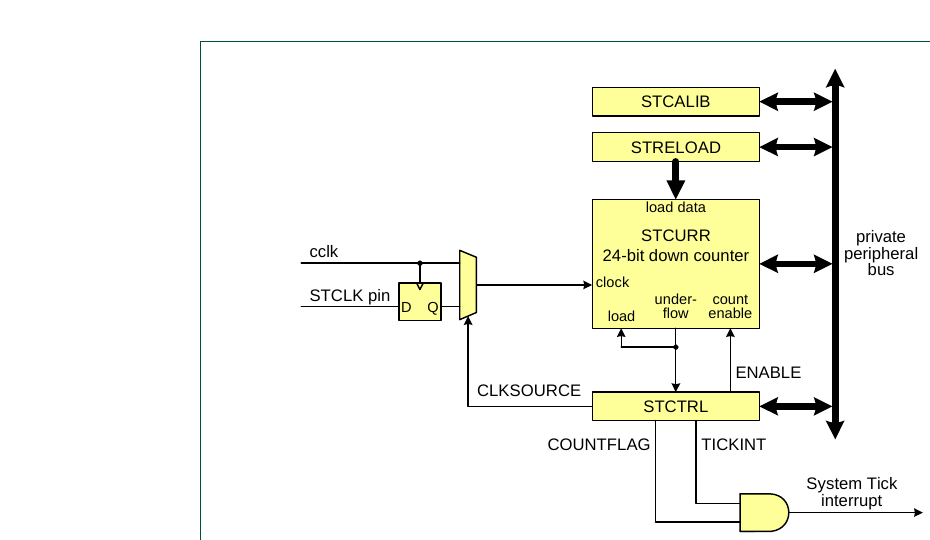
\includegraphics[width=0.90\textwidth]{images/lpc17xx_systick_block_diagram_fig118.png}
  \caption{System Tick Timer block diagram (Fig 118).}
\end{figure}

\paragraph{Nota t\'ecnica}
El flujo operativo real es: cargar \texttt{STRELOAD}, opcionalmente limpiar el contador escribiendo \texttt{STCURR}, configurar \texttt{STCTRL} y dejar que el contador recargue autom\'aticamente al llegar a cero. El bit \texttt{COUNTFLAG} se setea cuando ocurre ese underflow y se limpia al leer \texttt{STCTRL}.

\subsection{Register description}
\begin{table}[H]
  \centering
  \small
  \renewcommand{\arraystretch}{1.15}
  \caption{System Tick Timer register map (Table 438)}
  \begin{tabularx}{0.96\textwidth}{|>{\raggedright\arraybackslash}p{0.18\textwidth}|>{\raggedright\arraybackslash}X|>{\centering\arraybackslash}p{0.09\textwidth}|>{\centering\arraybackslash}p{0.14\textwidth}|>{\centering\arraybackslash}p{0.17\textwidth}|}
    \hline
    \textbf{Name} & \textbf{Description} & \textbf{Access} & \textbf{Reset value} & \textbf{Address} \\
    \hline
    \texttt{STCTRL} & System Timer Control and status register. & R/W & \texttt{0x4} & \texttt{0xE000 E010} \\
    \hline
    \texttt{STRELOAD} & System Timer Reload value register. & R/W & \texttt{0} & \texttt{0xE000 E014} \\
    \hline
    \texttt{STCURR} & System Timer Current value register. & R/W & \texttt{0} & \texttt{0xE000 E018} \\
    \hline
    \texttt{STCALIB} & System Timer Calibration value register. & R/W & \texttt{0x000F 423F} & \texttt{0xE000 E01C} \\
    \hline
  \end{tabularx}
\end{table}

\paragraph{Nota t\'ecnica}
El valor de reset reportado aplica a los \textbf{bits usados}. No debe interpretarse como contenido significativo en bits reservados.

\subsubsection{System Timer Control and status register (\texttt{STCTRL} - \texttt{0xE000 E010})}
\begin{table}[H]
  \centering
  \small
  \renewcommand{\arraystretch}{1.15}
  \caption{System Timer Control and status register (\texttt{STCTRL} - \texttt{0xE000 E010}) bit description (Table 439)}
  \begin{tabularx}{0.96\textwidth}{|>{\centering\arraybackslash}p{0.10\textwidth}|>{\raggedright\arraybackslash}p{0.18\textwidth}|>{\raggedright\arraybackslash}X|>{\centering\arraybackslash}p{0.12\textwidth}|}
    \hline
    \textbf{Bit} & \textbf{Symbol} & \textbf{Description} & \textbf{Reset value} \\
    \hline
    0 & \texttt{ENABLE} & Habilita el contador SysTick. \texttt{1}: contador habilitado. \texttt{0}: contador deshabilitado. & \texttt{0} \\
    \hline
    1 & \texttt{TICKINT} & Habilita la interrupci\'on del SysTick. Si vale \texttt{1}, la interrupci\'on se genera cuando el contador llega a \texttt{0}. & \texttt{0} \\
    \hline
    2 & \texttt{CLKSOURCE} & Selecci\'on de clock. \texttt{1}: \texttt{CPU clock}. \texttt{0}: pin externo \texttt{STCLK}. & \texttt{1} \\
    \hline
    15:3 & --- & Reservado. Software de usuario no debe escribir \texttt{1} en bits reservados. El valor le\'ido no est\'a definido. & \texttt{NA} \\
    \hline
    16 & \texttt{COUNTFLAG} & Flag que se setea cuando el contador llega a \texttt{0}. Se limpia al leer este registro. & \texttt{0} \\
    \hline
    31:17 & --- & Reservado. Software de usuario no debe escribir \texttt{1} en bits reservados. El valor le\'ido no est\'a definido. & \texttt{NA} \\
    \hline
  \end{tabularx}
\end{table}

\paragraph{Uso pr\'actico}
Si se usa como \textit{tick} peri\'odico, una configuraci\'on t\'ipica para clock interno es \texttt{ENABLE=1}, \texttt{TICKINT=1}, \texttt{CLKSOURCE=1}, lo que deja \texttt{STCTRL = 7}.

\subsubsection{System Timer Reload value register (\texttt{STRELOAD} - \texttt{0xE000 E014})}
\begin{table}[H]
  \centering
  \small
  \renewcommand{\arraystretch}{1.15}
  \caption{System Timer Reload value register (\texttt{STRELOAD} - \texttt{0xE000 E014}) bit description (Table 440)}
  \begin{tabularx}{0.96\textwidth}{|>{\centering\arraybackslash}p{0.10\textwidth}|>{\raggedright\arraybackslash}p{0.18\textwidth}|>{\raggedright\arraybackslash}X|>{\centering\arraybackslash}p{0.12\textwidth}|}
    \hline
    \textbf{Bit} & \textbf{Symbol} & \textbf{Description} & \textbf{Reset value} \\
    \hline
    23:0 & \texttt{RELOAD} & Valor que se carga en el contador SysTick cuando cuenta hacia abajo hasta \texttt{0}. & \texttt{0} \\
    \hline
    31:24 & --- & Reservado. Software de usuario no debe escribir \texttt{1} en bits reservados. El valor le\'ido no est\'a definido. & \texttt{NA} \\
    \hline
  \end{tabularx}
\end{table}

\subsubsection{System Timer Current value register (\texttt{STCURR} - \texttt{0xE000 E018})}
\begin{table}[H]
  \centering
  \small
  \renewcommand{\arraystretch}{1.15}
  \caption{System Timer Current value register (\texttt{STCURR} - \texttt{0xE000 E018}) bit description (Table 441)}
  \begin{tabularx}{0.96\textwidth}{|>{\centering\arraybackslash}p{0.10\textwidth}|>{\raggedright\arraybackslash}p{0.18\textwidth}|>{\raggedright\arraybackslash}X|>{\centering\arraybackslash}p{0.12\textwidth}|}
    \hline
    \textbf{Bit} & \textbf{Symbol} & \textbf{Description} & \textbf{Reset value} \\
    \hline
    23:0 & \texttt{CURRENT} & La lectura devuelve el valor actual del contador SysTick. Escribir cualquier valor limpia el contador SysTick y tambi\'en el bit \texttt{COUNTFLAG} en \texttt{STCTRL}. & \texttt{0} \\
    \hline
    31:24 & --- & Reservado. Software de usuario no debe escribir \texttt{1} en bits reservados. El valor le\'ido no est\'a definido. & \texttt{NA} \\
    \hline
  \end{tabularx}
\end{table}

\paragraph{Nota t\'ecnica}
\texttt{STCURR} no se usa para ``cargar'' un valor de arranque fino; para eso se usa \texttt{STRELOAD}. Su funci\'on operativa m\'as importante es permitir leer el conteo actual o forzar una limpieza del contador y del \texttt{COUNTFLAG}.

\subsubsection{System Timer Calibration value register (\texttt{STCALIB} - \texttt{0xE000 E01C})}
\begin{table}[H]
  \centering
  \small
  \renewcommand{\arraystretch}{1.15}
  \caption{System Timer Calibration value register (\texttt{STCALIB} - \texttt{0xE000 E01C}) bit description (Table 442)}
  \begin{tabularx}{0.96\textwidth}{|>{\centering\arraybackslash}p{0.10\textwidth}|>{\raggedright\arraybackslash}p{0.16\textwidth}|>{\raggedright\arraybackslash}p{0.18\textwidth}|>{\raggedright\arraybackslash}X|>{\centering\arraybackslash}p{0.12\textwidth}|}
    \hline
    \textbf{Bit} & \textbf{Symbol} & \textbf{Value} & \textbf{Description} & \textbf{Reset value} \\
    \hline
    23:0 & \texttt{TENMS} & --- & Valor de recarga para obtener un underflow SysTick cada \textbf{10 ms} cuando el clock es \textbf{100 MHz}. Los valores de \texttt{TENMS}, \texttt{SKEW} y \texttt{NOREF} aplican a ese caso de referencia. & \texttt{0x0F 423F} \\
    \hline
    29:24 & --- & --- & Reservado. Software de usuario no debe escribir \texttt{1} en bits reservados. El valor le\'ido no est\'a definido. & \texttt{NA} \\
    \hline
    30 & \texttt{SKEW} & --- & Indica si el valor de \texttt{TENMS} genera un intervalo exacto de \textbf{10 ms} o una aproximaci\'on. \texttt{0}: preciso. \texttt{1}: no preciso. & \texttt{0} \\
    \hline
    31 & \texttt{NOREF} & --- & Indica si existe clock de referencia externo separado. \texttt{0}: hay referencia separada disponible. \texttt{1}: no hay referencia separada. & \texttt{0} \\
    \hline
  \end{tabularx}
\end{table}

\paragraph{Nota t\'ecnica}
\texttt{STCALIB} no reemplaza el c\'alculo de \texttt{STRELOAD} para cualquier frecuencia arbitraria. Sirve como referencia de f\'abrica para el caso de \textbf{100 MHz}, que es el uso can\'onico que ARM asocia a SysTick.

\subsection{Example timer calculations}
\begin{table}[H]
  \centering
  \small
  \renewcommand{\arraystretch}{1.15}
  \caption{Resumen de c\'alculos de temporizaci\'on para \texttt{SysTick} a 10 ms}
  \begin{tabularx}{0.96\textwidth}{|>{\raggedright\arraybackslash}p{0.11\textwidth}|>{\raggedright\arraybackslash}p{0.22\textwidth}|>{\raggedright\arraybackslash}p{0.12\textwidth}|>{\raggedright\arraybackslash}p{0.19\textwidth}|>{\raggedright\arraybackslash}X|}
    \hline
    \textbf{Ejemplo} & \textbf{Clock} & \textbf{\texttt{STCTRL}} & \textbf{\texttt{RELOAD}} & \textbf{Observaci\'on} \\
    \hline
    1 & \texttt{CCLK = 100 MHz} & \texttt{7} & \texttt{999999 = 0xF423F} & Sin error de redondeo; coincide con el uso previsto del \texttt{STCALIB}. \\
    \hline
    2 & \texttt{CCLK = 80 MHz} & \texttt{7} & \texttt{799999 = 0xC34FF} & Sin error de redondeo; la precisi\'on depende de \texttt{CCLK}. \\
    \hline
    3 & \texttt{FIRC = 4 MHz} & \texttt{7} & \texttt{39999 = 0x9C3F} & Sin error de redondeo; la precisi\'on depende del \texttt{IRC}. \\
    \hline
    4 & \texttt{STCLK = 32.768 kHz} & \texttt{3} & \texttt{327 = 0x0147} & Hay error de redondeo; la frecuencia de interrupci\'on deriva levemente respecto del clock de entrada. \\
    \hline
  \end{tabularx}
\end{table}

\paragraph{Uso pr\'actico}
Para un per\'iodo objetivo de \textbf{10 ms}, la regla del manual es \texttt{RELOAD = (f / 100) - 1}. Cuando la frecuencia no es m\'ultiplo exacto de \texttt{100}, el resultado debe redondearse y eso introduce deriva temporal.
}{}

\end{document}
